\documentclass[b5paper]{book}
\usepackage[spanish]{babel}
\usepackage[latin1]{inputenc}
\usepackage{graphicx}
\special{pdf: pagesize width 17.6cm height 25.1cm}


\usepackage{fancyhdr}
\pagestyle{fancy}
\lfoot[\fancyplain{}{\thepage}]     {\fancyplain{}{}}
\cfoot[\fancyplain{}{}]     {\fancyplain{}{}}
\rfoot[\fancyplain{}{}]     {\fancyplain{}{\thepage}}


\title{Framework para el desarrollo de videojuegos}
\author{Javier Casas Velasco}
\date{No terminado}


%\voffset=-1.54cm


\evensidemargin=-0.54cm
\oddsidemargin=-1.04cm
\textwidth=14.1cm
\headwidth=14.1cm
%\usepackage[pdftex,
%        colorlinks=true,
%        urlcolor=rltblue,       % \href{...}{...} external (URL)
%        filecolor=rltgreen,     % \href{...} local file
%        linkcolor=rltred,       % \ref{...} and \pageref{...}
%        pdftitle={Untitled},
%        pdfauthor={Your Name},
%        pdfsubject={Just a test},
%        pdfkeywords={test, testing, testable stuff},
%        pdfproducer={pdfLaTeX},
%        pdfadjustspacing=1,
%        pagebackref,
%        pdfpagemode=None,
%        bookmarksopen=true]{hyperref}
%\usepackage{color}
%\definecolor{rltred}{rgb}{0.75,0,0}
%\definecolor{rltgreen}{rgb}{0,0.5,0}
%\definecolor{rltblue}{rgb}{0,0,0.75}


\begin{document}
\maketitle
\frontmatter
\tableofcontents
\mainmatter
%\input{funciones/funciones.tex}
%\part{Introducci�n}
%\chapter{Introducci�n}
Hasta ahora se ha especificado en general c�mo debe ser la forma y el comportamiento de las clases y del sistema. En este punto se discutir� al detalle c�mo debe ser implementado el sistema. Por ello, hasta este punto se ha estado hablando en t�rminos abstractos, en el c�mo deber�a funcionar. En este punto se especificar�n los mecanismos y detalles concretos que llevar� la implementaci�n.

\section{Restricciones y conversiones}
Para implementar este proyecto se utilizar� el lenguaje OCaML, que al igual que cualquier otro lenguaje de programaci�n tiene sus particularidades. Por ello, a continuaci�n se especifica una peque�a gu�a para transformar los modelos de an�lisis y dise�o a este lenguaje.

\begin{itemize}
\item \textbf{Tipos de dato}
	\begin{itemize}
	\item Void o vac�o, el tipo de dato que especifica que no se pasa nada de par�metro o no se devuelve nada, pasa a llamarse \emph{unit}.
	\item Conjunto ordenado, el tipo de dato que especifica una relaci�n con varias unidades siguiendo un determinado orden, pasa a ser \emph{array} o \emph{list}, dependiendo si es necesario el acceso r�pido a un elemento concreto o la capacidad de recorrer todos los elementos en orden.
	\item Conjunto, el tipo de dato que especifica una relaci�n con varias unidades, pasa a llamarse \emph{list}, por la facilidad de a�adir o filtrar elementos.
	\item Vector, Vector4, Vector3 y Vector2 son la misma clase con distintos nombres. La �nica diferencia reside en que si a Vector4, Vector3 o Vector2 se le pasa una cantidad de par�metros distinto al n�mero de la clase, se quejan y fallan con una excepci�n. Esto se hace con el fin de favorecer los controles de precondici�n y postcondici�n.
	\end{itemize}
\item \textbf{Operaciones del lenguaje}
	\begin{itemize}
	\item OCaML es un lenguaje fuertemente tipado, con inferencia de tipos. Debido a estas caracter�sticas, no es posible hacer \emph{downcasting}, es decir, transformar una referencia a una clase en una referencia a una de sus subclases. Esto se considera una operaci�n peligrosa y ambigua, y esa es la raz�n de que el lenguaje se niegue a implementarla.
	\item Debido a que el \emph{downcasting} es imposible, el \emph{upcasting} es una operaci�n de una s�la direcci�n, y no se puede invertir. Hay que crear caminos alternativos donde el \emph{downcasting} ser�a necesario.
	\item OCaML pone muchas trabas a la hora de crear dependencias circulares. Esto ha favorecido la creaci�n de un modelo de an�lisis y dise�o libre de dependencias circulares.
	\end{itemize}
\end{itemize}

%\part{Modelo de an�lisis}
%\chapter{Introducci�n}
Hasta ahora se ha especificado en general c�mo debe ser la forma y el comportamiento de las clases y del sistema. En este punto se discutir� al detalle c�mo debe ser implementado el sistema. Por ello, hasta este punto se ha estado hablando en t�rminos abstractos, en el c�mo deber�a funcionar. En este punto se especificar�n los mecanismos y detalles concretos que llevar� la implementaci�n.

\section{Restricciones y conversiones}
Para implementar este proyecto se utilizar� el lenguaje OCaML, que al igual que cualquier otro lenguaje de programaci�n tiene sus particularidades. Por ello, a continuaci�n se especifica una peque�a gu�a para transformar los modelos de an�lisis y dise�o a este lenguaje.

\begin{itemize}
\item \textbf{Tipos de dato}
	\begin{itemize}
	\item Void o vac�o, el tipo de dato que especifica que no se pasa nada de par�metro o no se devuelve nada, pasa a llamarse \emph{unit}.
	\item Conjunto ordenado, el tipo de dato que especifica una relaci�n con varias unidades siguiendo un determinado orden, pasa a ser \emph{array} o \emph{list}, dependiendo si es necesario el acceso r�pido a un elemento concreto o la capacidad de recorrer todos los elementos en orden.
	\item Conjunto, el tipo de dato que especifica una relaci�n con varias unidades, pasa a llamarse \emph{list}, por la facilidad de a�adir o filtrar elementos.
	\item Vector, Vector4, Vector3 y Vector2 son la misma clase con distintos nombres. La �nica diferencia reside en que si a Vector4, Vector3 o Vector2 se le pasa una cantidad de par�metros distinto al n�mero de la clase, se quejan y fallan con una excepci�n. Esto se hace con el fin de favorecer los controles de precondici�n y postcondici�n.
	\end{itemize}
\item \textbf{Operaciones del lenguaje}
	\begin{itemize}
	\item OCaML es un lenguaje fuertemente tipado, con inferencia de tipos. Debido a estas caracter�sticas, no es posible hacer \emph{downcasting}, es decir, transformar una referencia a una clase en una referencia a una de sus subclases. Esto se considera una operaci�n peligrosa y ambigua, y esa es la raz�n de que el lenguaje se niegue a implementarla.
	\item Debido a que el \emph{downcasting} es imposible, el \emph{upcasting} es una operaci�n de una s�la direcci�n, y no se puede invertir. Hay que crear caminos alternativos donde el \emph{downcasting} ser�a necesario.
	\item OCaML pone muchas trabas a la hora de crear dependencias circulares. Esto ha favorecido la creaci�n de un modelo de an�lisis y dise�o libre de dependencias circulares.
	\end{itemize}
\end{itemize}

%\chapter{Sistema actual}
Actualmente, el desarrollo profesional de juegos es una tarea muy compleja, ya que el uso de los �ltimos modelos de consolas de videojuegos significa una gran dificultad. Por ejemplo, las consolas PlayStation 3 y XBox 360 llevan en su interior un procesador Cell de 8 n�cleos de arquitectura RISC y dise�o SIMD. Esto significa que estas consolas pueden ejecutar simult�neamente 8 procesos del mismo programa y trabajar cada uno de estos procesos con multitud de datos simult�neamente. Esto significa, que para utilizar por completo la potencia de estas consolas es necesario un dise�o basado en partes separadas en procesos, con el fin de mantener ocupado lo m�s posible el procesador.

As�, hoy d�a es muy com�n dedicar un hilo a cada parte del programa que sea divisible. T�picamente, se dedica un hilo al procesamiento de la entrada, otro al de la l�gica del juego, otro a los gr�ficos, otro al sonido, otro a la red, etc. Esto significa que el juego debe ser dividido en partes separadas, y que puedan ser sincronizadas con la mayor facilidad y velocidad posibles. Esto ha favorecido la aparici�n de ingenios o motores dedicados a atender cada una de estas necesidades por separado, y que luego se integran en el desarrollo del juego.

%\chapter{Visi�n general}
Como ya se ha comentado, en este sistema pretendemos conseguir un mecanismo de aceleraci�n del desarrollo de un videojuego, ofreciendo para ello una parte del trabajo ya hecho. As� esa parte tan s�lo hay que retocarla y adaptarla al caso concreto. Por otra parte debe ser sencillo de manejar, con el fin de evitar que el coste de entrenar a los ingenieros para usarlo sea menor que el de desarrollar uno nuevo desde cero.

Por ello se busca que el sistema sea sencillo y extendible. Esto permitir� adaptarlo a los nuevos tiempos y a nuevas tecnolog�as. Esto implica que el sistema estar� desacoplado de bibliotecas concretas, con el fin de evitar que la desaparici�n de estas bibliotecas signifique el fin del sistema, y con la idea de poder adaptarlo a  bibliotecas nuevas.

Es evidente por lo indicado hasta ahora que este sistema est� orientado a desarrolladores.

En esta documentaci�n se distinguir� a dos tipos de usuarios:
\begin{itemize}
\item \textbf{El desarrollador} : Se le nombrar� normalmente como el usuario del producto, y es quien utiliza el sistema para desarrollar un videojuego.
\item \textbf{El jugador} : Es el usuario final, el que utiliza el videojuego desarrollado con el sistema que aqu� se expone.
\end{itemize}

\chapter{Requisitos funcionales}
\section{Introducci�n}
En este cap�tulo se describir� la funcionalidad de alto nivel del sistema.
\section{Requisitos del sistema en conjunto}
\begin{itemize}
\Requisito{1}{El sistema proporcionar� una ayuda al desarrollo de videojuegos.}{Imprescindible}{}
\Requisito{2}{El sistema proporcionar� un subsistema gr�fico listo para ser utilizado.}{Imprescindible}{}
\Requisito{3}{El sistema proporcionar� un subsistema de sonido listo para ser utilizado. En esta revisi�n no se incluye el desarrollo de dicho sistema.}{No implementado en esta revisi�n.}{}
\Requisito{4}{El sistema proporcionar� un subsistema de entrada listo para ser utilizado. En esta revisi�n no se incluye el desarrollo de dicho sistema.}{No implementado en esta revisi�n.}{}
\Requisito{5}{El sistema proporcionar� un esqueleto para facilitar la implementaci�n de la l�gica del juego.}{Imprescindible}{}
\Requisito{6}{El sistema proporcionar� el esqueleto t�pico de las aplicaciones interactivas.}{Imprescindible}{}
\end{itemize}

\section{Requisitos del subsistema gr�fico}
En esta secci�n nos referiremos al subsistema gr�fico como sistema gr�fico o motor gr�fico, para abreviar.

\begin{itemize}
\Requisito{2.1}{El motor gr�fico estar� orientado a las 3 dimensiones del espacio.}{Imprescindible}{}
\Requisito{2.2}{El motor gr�fico estar� organizado en torno al uso de pol�gonos como su estructura b�sica de representaci�n.}{Imprescindible}{}
	\begin{itemize}
	\Requisito{2.2.1}{Los pol�gonos soportar�n texturizado e iluminaci�n.}{Imprescindible}{}
	\Requisito{2.2.2}{El sistema proveer� un mecanismo para la importaci�n y carga de grandes grupos de pol�gonos (mallas).}{Imprescindible}{}
	\Requisito{2.2.3}{El motor gr�fico proveer� de una estructura b�sica para el manejo y procesamiento de mallas de pol�gonos.}{Imprescindible}{}
	\end{itemize}
\Requisito{2.3}{El motor gr�fico deber� ser f�cilmente desacoplable de la biblioteca gr�fica que se utilice.}{Imprescindible}{}
	\begin{itemize}
	\Requisito{2.3.1}{Inicialmente se utilizar� la biblioteca gr�fica OpenGL.}{Imprescindible}{}
	\end{itemize}
\Requisito{2.4}{El motor gr�fico tendr� disponibles entidades de alto nivel para su utilizaci�n.}{Imprescindible}{}
	\begin{itemize}
	\Requisito{2.4.1}{Una entidad de alto nivel ser� el objeto. Los objetos permitir�n manipular elementos de la escena como son c�maras y luces de una manera sencilla.}{Imprescindible}{}
	\Requisito{2.4.2}{Otra entidad de alto nivel ser� la pantalla. Las escenas agrupan objetos y se pintan en la pantalla, para que el jugador pueda verlas.}{Imprescindible}{}
	\end{itemize}
\Requisito{2.5}{El motor gr�fico estar� orientado a representar gr�ficos en tiempo real en la pantalla.}{Imprescindible}{}
\end{itemize}

%\section{Requisitos del subsistema de sonido}


%\section{Requisitos del subsistema de entrada}
%\begin{itemize}
%\Requisito{4.1}{El sistema proporcionar� un mecanismo para utilizar los dispositivos de entrada.}{Imprescindible}{}
%\Requisito{4.2}{El sistema simplificar� la utilizaci�n de los dispositivos de entrada.}{Imprescindible}{}
%	\begin{itemize}
%	\Requisito{4.2.1}{Existir� un tipo de dispositivo llamado binario, que en un determinado momento estar� o activado o desactivado.}{Imprescindible}{}
%	\Requisito{4.2.2}{Existir� un tipo de dispositivo llamado lineal, que en un determinado momento valdr� un valor en un intervalo.}{Imprescindible}{}
%	\Requisito{4.2.3}{Existir� un tipo de dispositivo llamado compuesto, y que ser� un agregado de otros dispositivos.}{Impresicindible}{}
%	\Requisito{4.2.4}{El sistema organizar� los dispositivos de entrada disponibles seg�n el esquema indicado anteriormente de dispositivos binarios, lineales y compuestos.}{Imprescindible}{}
%	\end{itemize}
%\end{itemize}


\section{Requisitos del esqueleto para la implementaci�n de la l�gica del juego}
\begin{itemize}
\Requisito{5.1}{El sistema proporcionar� un mecanismo para crear y procesar entidades concurrentes dentro del juego.}{Imprescindible}{}
\Requisito{5.2}{El sistema proporcionar� un mecanismo para el control eficiente y adecuado del tiempo dentro del juego.}{Alta}{}
\end{itemize}

\section{Requisitos del esqueleto de aplicaci�n interactiva}
\begin{itemize}
\Requisito{6.1}{El sistema proporcionar� un bucle principal.}{Imprescindible}{}
\Requisito{6.2}{El sistema estar� estructurado seg�n el modelo de bucle principal t�pico de aplicaci�n interactiva: 
	\begin{enumerate}
	\item Leer entrada
	\item Procesar informaci�n
	\item Representar resultados
	\item Ir a 1
	\end{enumerate} \ }{Imprescindible}{}
	
\end{itemize}

%\section{Requisitos del subsistema de entrada}
%A continuaci�n se enumeran los requisitos que tiene el sistema para aceptar entradas del jugador.
%\begin{enumerate}
%\item \ReqImprescindible{Interfaz de entrada}{El sistema debe proveer un subsistema capaz de leer entradas desde distinto hardware}{Ninguna}
%\item \ReqImprescindible{Teclado}{El sistema debe poder leer pulsaciones de teclas en el teclado en la forma ``pulsar tecla'' y ``soltar tecla'', con las limitaciones impuestas por el hardware}{Interfaz de entrada}
%\item \ReqImprescindible{Rat�n}{El sistema debe poder leer informaci�n disponible de uno o varios ratones o dispositivos equivalentes (trackball) en la forma ``pulsar bot�n'', ``soltar bot�n'', ``desplazamiento del rat�n'' y posiblemente ``lectura de ejes alternativos'' en el caso de que el rat�n disponga de ruletas u otros dispositivos}{Interfaz de entrada}
%\item \ReqImprescindible{Joypad}{El sistema debe poder leer informaci�n disponible de mandos de juegos en la forma ``posici�n de la palanca/cruceta'', ``pulsar bot�n'', ``soltar bot�n'' y ``posici�n de ejes alternativos''}{Interfaz de entrada}
%\item \ReqAlta{Otros dispositivos}{El sistema debe proveer mecanismos para la extensi�n y el soporte de nuevos mandos de entrada que aparezcan}{Intefaz de entrada}
%\item \ReqAlta{Unificaci�n del acceso}{El acceso a la informaci�n prove�da por los dispositivos debe ser lo m�s uniforme posible}{Ninguna}
%\item \ReqAlta{Demoras en el acceso}{El sistema debe implementar los mecanismos de acceso al hardware de entrada de una manera tal que la informaci�n se transfiera desde el hardware hasta la l�gica del juego con un retardo m�nimo}{Ninguna}
%\item \ReqAlta{Binding}{El enlace de datos entre el hardware y la l�gica del juego debe ser configurable en tiempo de ejecuci�n, con el fin garantizar la posibilidad de reconfigurar los controles en cualquier momento}{Ninguno}
%\end{enumerate}

%\section{Requisitos del subsistema de sonido}
%A continuaci�n se enumeran los requisitos dedicados a la parte sonora del sistema.
%
%\begin{enumerate}
%\item \ReqImprescindible{Sistema de sonido}{El sistema debe proveer un subsistema que pueda manejar y enviar sonidos a la tarjeta de sonido del sistema}{Ninguna}
%\end{enumerate}

%Con el fin de clasificar mejor estos requisitos se han agrupado en dos grupos: efectos de sonido y m�sica.

%\subsection{Efectos de sonido}
%\begin{enumerate}
%\item \ReqImprescindible{Efectos de sonido}{El sistema debe proveer un mecanismo para reproducir sonidos}{Sistema de sonido}
%\item \ReqImprescindible{Reproducci�n m�ltiple}{Los efectos de sonido se podr�n comenzar a reproducir a petici�n de la l�gica del juego en cualquier momento, pudiendo superponerse unos a otros}{Efectos de sonido}
%\item \ReqImprescindible{Control de volumen}{Debe proveerse un mecanismo que permita controlar el volumen de reproducci�n de un determinado efecto de sonido, con independencia de los dem�s efectos de sonido (inclu�das copias de �l mismo)}{Efectos de sonido}
%\item \ReqMedia{Velocidad de reproducci�n}{Debe existir un mecanismo que permita controlar la velocidad de reproducci�n de un efecto de sonido, con independencia de los dem�s efectos de sonido (inclu�das copias de �l mismo)}{Efectos de sonido}
%\item \ReqAlta{Est�reo o cuadraf�nico}{Debe haber un mecanismo que permita posicionar un sonido en el espacio con el fin de que suene adecuadamente en sistemas de altavoces en est�reo o cuadraf�nicos}{Efectos de sonido}
%\item \ReqAlta{Formatos est�ndar}{El sistema debe soportar la carga de efectos de sonido en la forma de sonidos con formato est�ndar}{Efectos de sonido}
%\end{enumerate}

%\subsection{M�sica}
%\begin{enumerate}
%\item \ReqImprescindible{M�sica}{El sistema debe proveer un mecanismo para reproducir m�sica}{Sistema de sonido}
%\item \ReqImprescindible{Control de reproducci�n}{El sistema de m�sica debe proveer un mecanismo para poder avanzar, parar, pausar, controlar el volumen o reproducir m�sica, siguiendo los conceptos que esto representar�a en un reproductor de CD}{M�sica}
%\item \ReqMedia{Reproducci�n m�ltiple}{El sistema debe poder reproducir varias m�sicas simult�neamente, y controlar cada una por separado de la manera que en el requisito \emph{Control de reproducci�n} se especifica }{M�sica}
%\item \ReqAlta{Carga diferida}{Debido a que el sistema no puede almacenar en memoria RAM gran cantidad de m�sica descomprimida, debe existir un mecanismo que cargue la m�sica en tiempo real de disco, a medida que se necesite}{M�sica}
%\item \ReqAlta{Formatos est�ndar}{El sistema debe soportar la carga de m�sica desde formatos est�ndar. Recomendados: MPEG Audio Layer-3 (MP3) y Ogg Vorbis (OGG)}{M�sica}
%\end{enumerate}


\chapter{Requisitos no funcionales}
\section{Facilidad de uso}
\section{Confiabilidad}
\begin{itemize}
\Requisito{N1}{El sistema debe estar implementado bajo unos modelos y unas pr�cticas que minimicen la necesidad de correcci�n de errores de implementaci�n en el futuro.}{Alta}{}
\end{itemize}

\section{Perfomance}
\begin{itemize}
\Requisito{N2}{El sistema debe ser r�pido en tiempo de ejecuci�n, y por tanto debe estar optimizado para funcionar lo m�s r�pido posible.}{Imprescindible}{}
\end{itemize}

\section{Restricciones de dise�o}
\begin{itemize}
\Requisito{N3}{El sistema debe estar dise�ado con la idea de poder portarlo con facilidad a otras arquitecturas o sistemas operativos.}{Imprescindible}{}
\end{itemize}

\section{Seguridad}
\begin{itemize}
\Requisito{N4}{El sistema debe ser resistente a ataques por parte de piratas inform�ticos ya sea local o remotamente.}{Medio}{}
\end{itemize}

\section{Documentaci�n de usuario y sistemas de ayuda}
\begin{itemize}
\Requisito{N5}{El sistema debe disponer de una documentaci�n de dise�o del mismo.}{Imprescindible}{}
\Requisito{N6}{El sistema debe disponer de una gu�a de funciones, objetos y clases que permitan a un desarrollador utilizarlo con facilidad.}{Imprescindible}{}
\end{itemize}

\section{Interfaces}
\subsection{Interfaces de usuario}
\begin{itemize}
\Requisito{N7.1}{El sistema debe proporcionar un interfaz para la visualizaci�n, audici�n e interactividad con el sistema.}{Imprescindible}{}
\end{itemize}
%\subsection{Interfaces Hardware}
\subsection{Interfaces Software}
\begin{itemize}
\Requisito{N7.2}{El sistema debe proporcionar un interfaz software que permita utilizarlo para desarrollar programas, es decir, debe ser integrable a un compilador y un generador de c�digo m�quina.}{Imprescindible}{}
\end{itemize}
%\subsection{Interfaces de comunicaci�n}


\newcommand{\flecha}[0]{-\textgreater\ }

\chapter{Modelos del sistema}
\section{Sistema gr�fico}
Se propone dividir el motor gr�fico en varios niveles, con el fin de simplificar las relaciones y reducir la dependencia. Por ello se proponen tres niveles:
\begin{itemize}
\item \textbf{Nivel de geometr�a} : Trata con v�rtices, pol�gonos y mallas
\item \textbf{Nivel de objetos} : Trata con los objetos que componen una escena, c�maras y luces
\item \textbf{Nivel de dibujado} : Trata de c�mo manejar las escenas que componen la imagen final que se muestra en pantalla
\end{itemize}



\subsection{Nivel de geometr�a}
Este nivel organiza el almacenamiento y proceso de las mallas de pol�gonos y los elementos que las componen. Est� organizado como clases de almacenamiento de datos (clases entidad) ya que apenas hay procesamiento en este subsistema, al menos respecto a la parte que ser� implementada en esta revisi�n.

\subsection{Nivel de objetos}
Este nivel organiza el procesamiento de las entidades que componen una escena, trat�ndolas como entidades indivisibles. Incluye el caso de uso \emph{emparentar}, que se encarga de describir c�mo unos objetos pueden depender de otros geom�tricamente hablando.

\subsection{Nivel de dibujado}
Este nivel se ha organizado para poder controlar varias pantallas con distintos sistemas e im�genes en cada una.

\section{Motor de procesos}
Este subsistema se encarga de proporcionar un esqueleto para la l�gica del juego. Para ello propone dividir dicha l�gica en peque�os elementos que se ejecutan concurrentemente como los procesos en un sistema operativo. Incluye los casos de uso \emph{ejecutar\_procesos}, que se encarga de dar tiempo de CPU a cada proceso; y \emph{cambiar\_prioridad}, que se encarga de decidir el orden en que se ejecutar�n los procesos.

\chapter{Escenarios}
\section{Sistema gr�fico}


\chapter{Modelo de casos de uso}
En este cap�tulo se describir�n los casos de uso principales.

\section{Descripciones generales de actores}
\begin{itemize}
\item \textbf{Desarrollador} : El desarrollador utiliza el sistema para desarrollar su videojuego.
\item \textbf{Usuario} : El usuario en un caso de uso suele ser el propio software a�adido por el desarrollador para utilizar el framework. A menudo tambi�n ser� cualquier otra parte del sistema que dependa de la que se est� describiendo actualmente. En esos casos en la descripci�n del caso de uso se indicar� qui�n es un buen candidato a usar el sistema.
\item \textbf{Main Loop} : A menudo, el bucle principal de la aplicaci�n iniciar� un caso de uso.
\item \textbf{Proceso} : Muchas veces, parte de la l�gica del juego, expresada como procesos, iniciar� un caso de uso.
\end{itemize}
\section{Diagrama de modelo de casos de uso}

\section{General: bucle principal}
El modelo de ejecuci�n general del programa. Est� basado en el modelo de ejecuci�n de un programa interactivo, adaptado para este sistema.
\subsection{Flujo b�sico}
\begin{enumerate}
\item El sistema se inicializa.
\item Mientras deba continuar la ejecuci�n del sistema:
	\begin{enumerate}
	\item El jugador genera eventos de entrada si desea.
	\item Si hay eventos de entrada:
		\begin{enumerate}
		\item El sistema procesa los eventos de entrada.
		\end{enumerate}
	\item El sistema procesa la informaci�n del juego.
	\item El sistema muestra el resultado del procesamiento.
	\item El jugador ve el resultado de sus acciones.
	\end{enumerate}
\item El sistema libera recursos y finaliza su ejecuci�n.
\end{enumerate}
\subsection{Requisitos especiales}
\subsection{Precondiciones}
\subsection{Postcondiciones}
\subsection{Puntos de extensi�n}
\subsection{Relaciones}
\subsection{Otros diagramas}


\section{Objetos: emparentar objeto}
Cambia de padre a un objeto. Sirve para desplazar ese objeto por el �rbol de objetos.
\subsection{Flujo b�sico}
\begin{enumerate}
\item El usuario ordena al objeto cambiar de padre, y especifica un nuevo padre.
\item Si el objeto ten�a otro padre anteriormente:
	\begin{enumerate}
	\item El objeto se libera de la dependencia con su padre anterior.
	\end{enumerate}
\item El objeto establece una dependencia con su nuevo padre.
\end{enumerate}

\subsection{Requisitos especiales}
\subsection{Precondiciones}
\subsection{Postcondiciones}
\subsection{Puntos de extensi�n}
\subsection{Relaciones}
\subsection{Otros diagramas}

\chapter{Modelos Objeto}
\section{Nivel de geometr�a}
Este nivel se ha propuesto principalmente como un mecanismo para almacenar y procesar geometr�a, y ha sido organizado seg�n el modelo de datos de almacenamiento de geometr�a. En los sistemas m�s sencillos, la geometr�a a nivel de pol�gono tan solo debe ser consultada para pintarla en pantalla. Por ello no se contemplan operaciones complejas y raras, como pueden ser deformaciones din�micas y operaciones CSG (Geometr�a S�lida Constructiva).

\begin{figure}[htp]
\centering
%\includegraphics[width=14cm]{analisis/propuesto/modelos_objeto/geometria/clases.eps}
\includegraphics[width=14cm]{diagramas/analisis/geometria-clases.eps}
\caption{Diagrama de clases de an�lisis del nivel de Geometr�a}
\end{figure}


A�n as�, este es el modelo abstracto, y puede ser extendido para soportar otras operaciones.
A continuaci�n se describir� la utilidad de cada clase:

\subsection{Coordenada}
Almacena una coordenada en el espacio 3D.
\begin{itemize}
\item \textbf{Responsabilidades:}
	\begin{itemize}
	\item Almacenar una coordenada del espacio.
	\end{itemize}
\item \textbf{Relaciones:}
	\begin{itemize}
	\item -valor : vector3 \newline
		Vector con las coordenadas almacenadas.
	\end{itemize}
\item \textbf{M�todos:}
	\begin{itemize}
	\item \emph{+creaci�n}(v:vector3) : coordenada \newline
		Hace una coordenada nueva con valor v.
	\item +valor() : vector3 \newline
		Vector con las coordenadas almacenadas.
	\end{itemize}
\end{itemize}

\subsection{Normal}
Almacena una direcci�n normal.
\begin{itemize}
\item \textbf{Responsabilidades:}
	\begin{itemize}
	\item Almacenar una direcci�n normal.
	\item Mantener dicha direcci�n normal unitaria (vector de longitud 1).
	\end{itemize}
\item \textbf{Relaciones:}
	\begin{itemize}
	\item -valor : vector3 \newline
		Vector con la normal almacenada.
	\end{itemize}
\item \textbf{M�todos:}
	\begin{itemize}
	\item \emph{+creaci�n}(v:vector3) : normal \newline
		Hace una normal nueva con valor v.
	\item +valor() : vector3 \newline
		Vector con la normal.
	\end{itemize}
\end{itemize}

\subsection{Color}
Almacena un color. El color se almacena en formato RGBA, esto es, las componentes de los vectores representan los colores en orden Rojo, Verde, Azul, Alfa, donde Alfa es el valor de transparencia. Los valores pueden variar en el intervalo [0..1], donde 0 es intensidad nula y 1 es intensidad m�xima. Para el valor de Alfa, 1 significa completamente opaco y 0 significa completamente transparente.
\begin{itemize}
\item \textbf{Responsabilidades:}
	\begin{itemize}
	\item Almacenar un color.
	\item Almacenar un valor de transparencia.
	\end{itemize}
\item \textbf{Relaciones:}
	\begin{itemize}
	\item -valor : vector4 \newline
		Vector con el color en formato RGBA.
	\end{itemize}
\item \textbf{M�todos:}
	\begin{itemize}
	\item \emph{+creaci�n}(v:vector4) : color \newline
		Hace un color nuevo con valor v.
	\item +valor() : vector4 \newline
		Vector con el color en formato RGBA.
	\end{itemize}
\end{itemize}

\subsection{UV}
Almacena una coordenada UV o de texturizado.

Restricci�n: Para cada v�rtice de un determinado pol�gono debe haber tantas coordenadas UV como capas tenga el pol�gono.

\begin{itemize}
\item \textbf{Responsabilidades:}
	\begin{itemize}
	\item Almacenar una coordenada de texturizado.
	\end{itemize}
\item \textbf{Relaciones:}
	\begin{itemize}
	\item -valor : vector2 \newline
		Vector con la coordenada UV.
	\end{itemize}
\item \textbf{M�todos:}
	\begin{itemize}
	\item \emph{+creaci�n}(v:vector2) : UV \newline
		Hace una UV nueva con valor v.
	\item +valor() : vector2 \newline
		Vector con la coordenada UV.
	\end{itemize}
\end{itemize}

\subsection{Material}
Almacena el material del que est� compuesta la suerficie de un pol�gono.
\begin{itemize}
\item \textbf{Responsabilidades:}
	\begin{itemize}
	\item Almacenar informaci�n de un material.
	\end{itemize}
\item \textbf{Relaciones:}
	\begin{itemize}
	\item -textura : textura \newline
		El mapa de bits que utiliza de textura
	\end{itemize}
\item \textbf{M�todos:}
	\begin{itemize}
	\item \emph{+creaci�n}(t:textura) : material \newline
		Hace un material nuevo con la textura t.
	\item +textura() : textura \newline
		El mapa de bits que utiliza de textura.
	\end{itemize}
\end{itemize}

\subsection{V�rtice}
Almacena un v�rtice de un pol�gono.
\begin{itemize}
\item \textbf{Responsabilidades:}
	\begin{itemize}
	\item Almacenar un v�rtice, con sus coordenadas, su posici�n de texturizado y la direcci�n normal de la superficie en ese punto.
	\end{itemize}
\item \textbf{Relaciones:}
	\begin{itemize}
	\item -coordenada : coordenada \newline
		La posici�n del v�rtice dentro del espacio.
	\item -normal : normal \newline
		La direcci�n normal del v�rtice.
	\item -color : color \newline
		El color del v�rtice.
	\item -uvs : colecci�n ordenada de UV \newline
		Las coordenadas UV de texturizado del v�rtice.
	\end{itemize}
\item \textbf{M�todos:}
	\begin{itemize}
	\item \emph{+creaci�n}(c:coordenada, n:normal, co:color, uvs:colecci�n ordenada de uv) : vertice \newline
		Hace un nuevo v�rtice con las caracter�sticas indicadas.
	\item +coordenada() : coordenada \newline
		La posici�n del v�rtice dentro del espacio.
	\item +normal() : normal \newline
		La direcci�n normal del v�rtice.
	\item +color() : color \newline
		El color del v�rtice.
	\item +uv(n:entero) : UV \newline
		Las coordenadas UV de texturizado del v�rtice, referidas a la capa n.
	\end{itemize}
\end{itemize}

\subsection{Capa}
Almacena la informaci�n referida a una capa que se aplica a un pol�gono.
\begin{itemize}
\item \textbf{Responsabilidades:}
	\begin{itemize}
	\item Almacenar informaci�n sobre una capa de pintado que se aplica sobre un conjunto de pol�gonos.
	\end{itemize}
\item \textbf{Relaciones:}
	\begin{itemize}
	\item -material : material \newline
		El material asociado a la capa.
	\end{itemize}
\item \textbf{M�todos:}
	\begin{itemize}
	\item \emph{+creaci�n}(m:material) : capa \newline
		Hace una nueva capa con material m.
	\item +material() : material \newline
		El material asociado a la capa.
	\end{itemize}
\end{itemize}

\subsection{Pol�gono}
Almacena la informaci�n de un pol�gono.

Restricci�n: Para cada v�rtice de un pol�gono debe haber tantas coordenadas UV como capas tenga el pol�gono.


\begin{itemize}
\item \textbf{Responsabilidades:}
	\begin{itemize}
	\item Almacenar los v�rtices y las capas de material de un pol�gono.
	\end{itemize}
\item \textbf{Relaciones:}
	\begin{itemize}
	\item -v�rtices : colecci�n ordenada de v�rtice \newline
		Los v�rtices del pol�gono.
	\item -capas : colecci�n ordenada de capa \newline
		Las capas de pintado que se aplican al pol�gono.
	\end{itemize}
\item \textbf{M�todos:}
	\begin{itemize}
	\item \emph{+creaci�n}(v:colecci�n ordenada de v�rtice, c:colecci�n ordenada de capa) : pol�gono \newline
		Hace un nuevo pol�gono con v�rtices v y capas c.
	\item +v�rtice(n:entero) : v�rtice \newline
		El n-�simo v�rtice.
	\item +capa(n:entero) : capa \newline
		La n-�sima capa.
	\end{itemize}
\end{itemize}

\subsection{Malla}
Almacena una malla de pol�gonos.
\begin{itemize}
\item \textbf{Responsabilidades:}
	\begin{itemize}
	\item Almacenar una malla de pol�gonos.
	\end{itemize}
\item \textbf{Relaciones:}
	\begin{itemize}
	\item -pol�gonos : colecci�n de pol�gono \newline
		Los pol�gonos de la malla.
	\end{itemize}
\item \textbf{M�todos:}
	\begin{itemize}
	\item \emph{+creaci�n}(p:colecci�n de pol�gono) : malla \newline
		Hace una nueva malla con los pol�gonos p.
	\item +pol�gonos() : colecci�n de pol�gono \newline
		Los pol�gonos de la malla.
	\end{itemize}
\end{itemize}



\section{Nivel de objetos}
Este nivel se ha propuesto con el fin de almacenar y ordenar adecuadamente los objetos. Por ello se propone organizarlos en forma de �rbol, donde la ra�z sea el punto de control y acceso del �rbol entero. Adem�s se utiliza esto para dar un significado extra a los objetos. La transformada de un objeto utiliza como origen de coordenadas las del objeto inmediatamente superior en el �rbol, que a su vez utiliza las del objeto superior, etc. Esto es cierto para todos los objetos excepto el objeto origen, que representa el origen de coordenadas del espacio. Esta caracter�stica permite implementar la capacidad de \emph{pegar} unos objetos a otros. El objeto \emph{pegado} pasar�a a ser descendiente del objeto al que ha sido pegado, y as�, al ejercer una transformada sobre el objeto padre el objeto pegado le seguir�a, \emph{pegado} a sus coordenadas locales.

\begin{figure}[htp]
\centering
%\includegraphics[width=14cm]{analisis/propuesto/modelos_objeto/objetos/clases.eps}
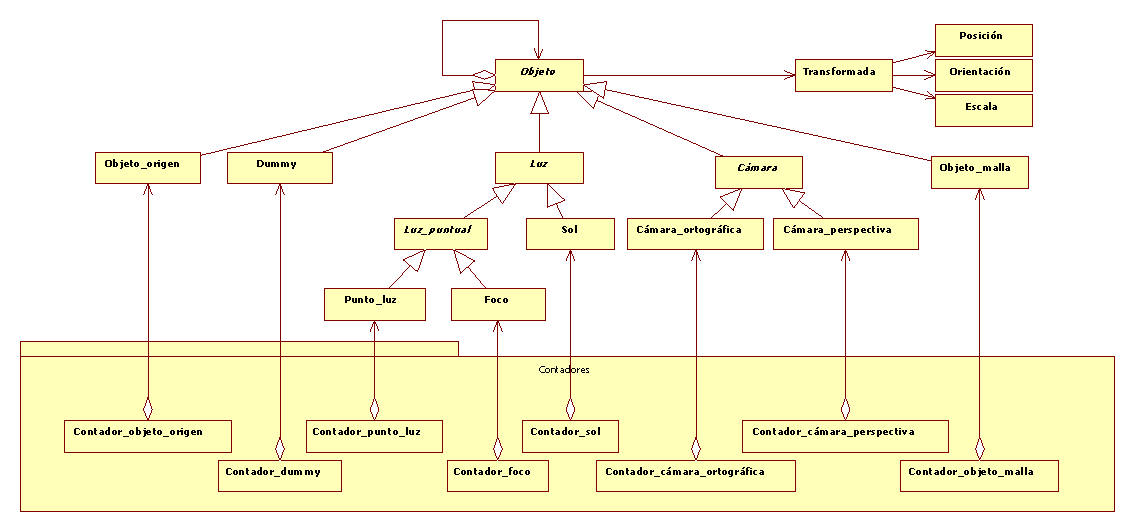
\includegraphics[width=14cm]{diagramas/analisis/objetos-clases.eps}

\caption{Diagrama de clases de an�lisis del nivel de Objetos}
\end{figure}


A continuaci�n se describe la utilidad de cada clase:

\subsection{Posici�n}
Almacena la indicaci�n de un lugar en el espacio.
\begin{itemize}
\item \textbf{Responsabilidades:}
	\begin{itemize}
	\item Almacenar una coordenada relativa en el espacio 3D.
	\item Proveer mecanismos para manipular esa coordenada.
	\end{itemize}
\item \textbf{Relaciones:}
	\begin{itemize}
	\item -coordenadas : vector3 \newline
		Coordenadas indicando la posici�n.
	\end{itemize}
\item \textbf{M�todos:}
	\begin{itemize}
	\item \emph{+creaci�n}() : posici�n \newline
		Hace una nueva posici�n situada en el origen relativo (coordenadas 0,0,0).
	\item +coordenadas() : vector3 \newline
		Las coordenadas que indican la posici�n.
	\item +mover(desplazamiento:vector3)\newline
		Mueve la posici�n la cantidad indicada.
	\item +establecer\_posici�n(p:vector3)\newline
		Sit�a la posici�n en el lugar indicado.
	\end{itemize}
\end{itemize}

\subsection{Orientaci�n}
Almacena una rotaci�n en el espacio. Hay que remarcar que la orientaci�n se puede especificar mediante dos vectores: uno que indica a d�nde apunta y otro que indica la vertical. Como vectores originales se propone (1,0,0) para la direcci�n de apunte y (0,1,0) para la vertical de un objeto que no ha sido rotado. No hay m�todos para rotaciones de Euler, pero se recuerda que estas se pueden obtener mediante una sucesi�n de tres rotaciones alrededor de los ejes xyz o zyx.
\begin{itemize}
\item \textbf{Responsabilidades:}
	\begin{itemize}
	\item Almacenar una rotaci�n en el espacio 3D.
	\item Proveer mecanismos para manipular esa rotaci�n.
	\end{itemize}
\item \textbf{Relaciones:}
	\begin{itemize}
	\item -valor : cuaterni�n \newline
		Cuaterni�n con la rotaci�n.
	\end{itemize}
\item \textbf{M�todos:}
	\begin{itemize}
	\item \emph{+creaci�n}() : orientaci�n \newline
		Hace una nueva orientaci�n nula (sin orientaci�n inicial).
	\item +rotar(v:vector3, angulo:float)\newline
		Rota la orientaci�n alrededor del vector especificado el �ngulo especificado (en grados).
	\item +establecer\_rotaci�n(v:vector3, angulo:float) \newline
		Modifica la orientaci�n para que tenga las caracter�sticas indicadas.
	\item +extraer\_rotaci�n() : (v:vector3, angulo:float) \newline
		Devuelve la orientaci�n como una �nica rotaci�n.
	\item +frontal() : vector3 \newline
		Devuelve la direcci�n a la que apunta la orientaci�n.
	\item +vertical() : vector3 \newline
		Devuelve la direcci�n vertical de la orientaci�n.
	\item +rotar\_vector(vector3) : vector3 \newline
		Aplica la orientaci�n al vector indicado.
	\end{itemize}
\end{itemize}

\subsection{Escala}
Almacena las dimensiones de forma relativa. Es decir, para un objeto, las dimensiones (1,1,1) corresponden a su tama�o original, mientras que (10,10,10) corresponder�a a un objeto 10 veces m�s grande en cada una de sus dimensiones. Se soportan dimensiones negativas, que significan que el objeto est� reflejado en el eje indicado. Tambi�n se soportan dimensiones nulas, que significan que el objeto est� proyectado sobre un subespacio de dimensi�n inferior. Esto debe ser tenido en cuenta por la implementaci�n concreta bajo un API concreto del motor gr�fico.
\begin{itemize}
\item \textbf{Responsabilidades:}
	\begin{itemize}
	\item Almacenar una definici�n de escala relativa en el espacio 3D.
	\item Proveer mecanismos para manipular esa definici�n de escala.
	\end{itemize}
\item \textbf{Relaciones:}
	\begin{itemize}
	\item -valor : vector3 \newline
		Vector con las tres dimensiones.
	\end{itemize}
\item \textbf{M�todos:}
	\begin{itemize}
	\item \emph{+creaci�n}() : escala \newline
		Hace una nueva escala con tama�o original (1,1,1).
	\item +escalar(vector3) \newline
		Multiplica el vector escala por el indicado, elemento a elemento y almacena el resultado.
	\item +establecer\_escala(vector3)\newline
		Modifica la escala para que tenga las caracter�sticas indicadas.
	\item +escala() : vector3 \newline
		Devuelve un vector con las tres componentes de la escala.
	\end{itemize}
\end{itemize}

\subsection{Transformada}
Almacena una transformada de un objeto. S�lo se almacenan la posici�n, orientaci�n y escala del objeto. Como se indic� antes, estas transformadas se almacenan relativamente respecto al objeto padre.
\begin{itemize}
\item \textbf{Responsabilidades:}
	\begin{itemize}
	\item Almacenar una definici�n de transformada relativa en el espacio 3D.
	\item La transformada debe soportar desplazamientos, rotaciones y escalas.
	\item Proveer mecanismos para manipular esa transformada.
	\end{itemize}
\item \textbf{Relaciones:}
	\begin{itemize}
	\item -posici�n : posici�n \newline
	\item -orientaci�n : orientaci�n \newline
	\item -escala : escala \newline
	\end{itemize}
\item \textbf{M�todos:}
	\begin{itemize}
	\item \emph{+creaci�n}() : transformada \newline
		Hace una nueva transformada. Esta transformada tiene las siguientes caracter�sticas:
		\begin{itemize}
		\item Posici�n: (0,0,0)
		\item Orientaci�n: Vector(1,0,0), �ngulo 0�
		\item Escala: (1,1,1)
		\end{itemize}
	\item +posici�n() : posici�n \newline
		La posici�n.
	\item +orientaci�n() : orientaci�n \newline
		La orientaci�n.
	\item +escala() : escala \newline
		La escala.
	\end{itemize}
\end{itemize}

\subsection{Objeto}
Almacena un objeto en el espacio. Esta clase es el modelo abstracto para acceder al �rbol de objetos que representa una escena, y de ella heredan los tipos concretos de objeto que se describir�n.
\begin{itemize}
\item \textbf{Responsabilidades:}
	\begin{itemize}
	\item Almacenar y organizar un objeto en el espacio.
	\item Proveer un mecanismo para la organizaci�n de objetos en forma de �rbol.
	\end{itemize}
\item \textbf{Relaciones:}
	\begin{itemize}
	\item \#padre : objeto opcional \newline
		El objeto inmediatamente superior en el �rbol de objetos (si est� metido en un �rbol de objetos).
	\item \#hijos : colecci�n de objeto \newline
		Los objetos que tienen a este objeto de padre.
	\item \#transformada : transformada \newline
		La transformada de este objeto.
	\end{itemize}
%\item \textbf{Atributos:}
%	\begin{itemize}
%	\end{itemize}
\item \textbf{M�todos:}
	\begin{itemize}
	\item \emph{+creaci�n}() : objeto \newline
		Crea el objeto nuevo e inicializa la tranformada.
	\item +padre() : objeto\newline
		El padre del objeto.
	\item \#set\_padre(objeto opcional)\newline
		Cambia el atributo \emph{padre}
	\item +hijos() : colecci�n de objeto\newline
		Los objetos hijo.
	\item \#set\_hijos(colecci�n de objeto)\newline
		Cambia el atributo \emph{hijos}
	\item +establecer\_padre(objeto)\newline
		Hace que el objeto indicado pase a ser el padre de este objeto, y este objeto pase a ser hijo del objeto indicado. Elimina otras dependencias con otros objetos si existieran.
	\item +origen() : objeto \newline
		El objeto origen del que depende el �rbol donde est� situado este objeto.
	\item +transformada() : transformada \newline
		Devuelve la transformada del objeto.
	\item +transformada\_final() : transformada \newline
		Computa la transformada desde el origen hasta el objeto actual, obteniendo una transformada que ser�a el resultado de aplicar cada una de las transformadas que afectan al objeto en orden.
	\end{itemize}
\end{itemize}

\subsection{Objeto\_origen}
Almacena el origen de coordenadas del espacio como objeto. Est� pensado para ser la ra�z del �rbol de objetos. Ya que todos los objetos dependen posicionalmente de �ste no tiene sentido modificar su transformada (todos los objetos, incluida la c�mara se ver�an afectados igual, y la escena no cambiar�a desde el punto de vista del observador).
\begin{itemize}
\item \textbf{Responsabilidades:}
	\begin{itemize}
	\item Proveer una ra�z para el �rbol de objetos.
	\end{itemize}
\item \textbf{Relaciones:}
	\begin{itemize}
	\item Es una especificaci�n de Objeto. \newline
		Es un tipo de objeto pensado para ser la ra�z del �rbol de objetos.
	\end{itemize}
\item \textbf{M�todos:}
	\begin{itemize}
	\item \emph{+creaci�n}() : objeto\_origen \newline
		Crea un objeto\_origen nuevo.
	\end{itemize}
\end{itemize}

\subsection{Dummy}
El dummy es un objeto nulo, que no afecta a la representaci�n en la pantalla. Sin embargo, puede ser utilizado para pegarle otros objetos y manipularlos en conjunto a trav�s de �ste.
\begin{itemize}
\item \textbf{Responsabilidades:}
	\begin{itemize}
	\item Proveer un objeto que no afecte a la representaci�n en la pantalla, pero pueda ser utilizado como punto de apoyo.
	\end{itemize}
\item \textbf{Relaciones:}
	\begin{itemize}
	\item Es una especificaci�n de Objeto. \newline
		Es un tipo de objeto pensado para ser la ra�z de sub-�rboles de objetos.
	\end{itemize}
\item \textbf{M�todos:}
	\begin{itemize}
	\item \emph{+creaci�n}() : dummy \newline
		Crea un dummy nuevo.
	\end{itemize}
\end{itemize}

\subsection{Luz}
Representa una fuente de luz que ilumina la escena. Tiene varias especializaciones que se especifican m�s adelante. Cabe resaltar que el color tambi�n especifica la \emph{cantidad} de luz. As�, una luz de color (1.0, 1.0, 1.0) es blanca de intensidad m�xima, mientras que una luz de color (0.5, 0.5, 0.5) tambi�n es blanca, pero de intensidad media. Una luz \emph{apagada} (que realmente no emite luz) tendr�a un color (0.0, 0.0, 0.0). La luz se divide en dos partes: difusa y especular. La parte difusa se refleja uniformemente en todas las direcciones. En cambio, la parte especular se refleja preferentemente en direcciones concretas, de una manera similar a como la luz se refleja en un espejo o una superficie pulida.
\begin{itemize}
\item \textbf{Responsabilidades:}
	\begin{itemize}
	\item Proveer un objeto que represente una fuente de luz.
	\end{itemize}
\item \textbf{Relaciones:}
	\begin{itemize}
	\item Es una especificaci�n de Objeto. \newline
		Es un tipo de objeto que representa una fuente de luz.
	\item \#color\_difuso : color \newline
		El color de la parte difusa de la luz
	\item \#color\_especular : color \newline
		El color de la parte especular de la luz
	\end{itemize}
\item \textbf{M�todos:}
	\begin{itemize}
	\item \emph{+creaci�n}() : luz \newline
		Inicializa la luz a valores por defecto. Estos son:
		\begin{itemize}
		\item Color difuso : (1.0,1.0,1.0)
		\item Color especular : (0.0,0.0,0.0)
		\end{itemize}
	\item +color\_difuso() : color \newline
		El color de la parte difusa de la luz
	\item +set\_color\_difuso(color)\newline
		Cambia el color difuso de la luz.
	\item +color\_especular() : color \newline
		El color de la parte especular de la luz
	\item +set\_color\_especular(color) \newline
		Cambia el color especular de la luz.
	\end{itemize}
\end{itemize}

\subsection{Luz\_puntual}
Representa una fuente de luz que sale de un punto del espacio. El factor de atenuaci�n se computa como:

\begin{displaymath}
Atenuaci\acute on = \frac{1}{Kc + Kl*d + Kq*d^2}
\end{displaymath}
Donde $Kc$ es el factor de atenuaci�n constante, $Kl$ es el factor de atenuaci�n lineal, $Kq$ es el factor de atenuaci�n cuadr�tico y $d$ es la distancia del punto de luz al v�rtice iluminado.

\begin{itemize}
\item \textbf{Responsabilidades:}
	\begin{itemize}
	\item Proveer un objeto que represente una fuente de luz puntual.
	\end{itemize}
\item \textbf{Relaciones:}
	\begin{itemize}
	\item Es una especificaci�n de Luz. \newline
		Es un tipo de Luz que representa al grupo de luces que proceden de un punto en el espacio.
	\end{itemize}
\item \textbf{Atributos:}
	\begin{itemize}
	\item \#atenuacion\_constante : real \newline
		El factor de atenuaci�n de la luz constante
	\item \#atenuacion\_lineal : real \newline
		El factor de atenuaci�n de la luz que depende linealmente de la distancia del punto de luz al v�rtice iluminado.
	\item \#atenuacion\_cuadr�tica : real \newline
		El factor de atenuaci�n de la luz que depende cuadr�ticamente de la distancia del punto de luz al v�rtice iluminado.
	\end{itemize}
\item \textbf{M�todos:}
	\begin{itemize}
	\item \emph{+creaci�n}() : luz\_puntual \newline
		Inicializa la luz con los valores:
		\begin{itemize}
		\item Atenuaci�n constante : 1
		\item Atenuaci�n lineal : 0
		\item Atenuaci�n cuadr�tica : 0
		\end{itemize}
	\item +atenuacion\_constante() : real \newline
		El factor de atenuaci�n de la luz constante
	\item +set\_atenuacion\_constante(real)\newline
		Cambia el factor de atenuaci�n de la luz constante
	\item +atenuacion\_lineal() : real \newline
		El factor de atenuaci�n de la luz que depende linealmente de la distancia del punto de luz al v�rtice iluminado.
	\item +set\_atenuacion\_lineal(real) \newline
		Cambia el factor de atenuaci�n de la luz que depende linealmente de la distancia del punto de luz al v�rtice iluminado.
	\item +atenuacion\_cuadr�tica() : real \newline
		El factor de atenuaci�n de la luz que depende cuadr�ticamente de la distancia del punto de luz al v�rtice iluminado.
	\item +set\_atenuacion\_cuadr�tica(real)\newline
		Cambia el factor de atenuaci�n de la luz que depende cuadr�ticamente de la distancia del punto de luz al v�rtice iluminado.
	\end{itemize}
\end{itemize}

\subsection{Punto\_luz}
Representa una fuente de luz puntual omnidireccional, es decir, que la luz se emite uniformemente en todas las direcciones.
\begin{itemize}
\item \textbf{Responsabilidades:}
	\begin{itemize}
	\item Proveer un objeto que represente una fuente de luz puntual.
	\end{itemize}
\item \textbf{Relaciones:}
	\begin{itemize}
	\item Es una especificaci�n de Luz\_puntual. \newline
		Es una luz puntual que radia por igual en todas direcciones.
	\end{itemize}
\item \textbf{M�todos:}
	\begin{itemize}
	\item \emph{+creaci�n}() : punto\_luz \newline
		Crea un punto\_luz nuevo.
	\end{itemize}
\end{itemize}

\subsection{Foco}
Representa una fuente de luz puntual con una direcci�n preferente de iluminaci�n. El foco ilumina en la direcci�n frontal a la que apunta su transformada.
\begin{itemize}
\item \textbf{Responsabilidades:}
	\begin{itemize}
	\item Proveer un objeto que represente una fuente de luz direccional
	\end{itemize}
\item \textbf{Relaciones:}
	\begin{itemize}
	\item Es una especificaci�n de Luz\_puntual. \newline
		Es una luz puntual que radia en una direcci�n concreta.
	\end{itemize}
\item \textbf{Atributos:}
	\begin{itemize}
	\item \#apertura : real \newline
		Especifica el �ngulo de apertura del cono de luz. Intervalo v�lido: [0�,90�]
	\item \#concentraci�n : real \newline
		Especifica la concentraci�n de luz. Valores peque�os significan que la luz se distribuye uniformemente, mientras que valores grandes significan que la luz se concentra en el centro del foco. Intervalo v�lido [0,100]
	\end{itemize}
\item \textbf{M�todos:}
	\begin{itemize}
	\item \emph{+creaci�n}() : foco \newline
		Crea e inicializa el foco con los valores siguientes:
		\begin{itemize}
		\item Apertura : 45�
		\item Concentraci�n : 0
		\end{itemize}
	\item +apertura() : real \newline
		El �ngulo de apertura del cono de luz.
	\item +set\_apertura(real)\newline
		Cambia el �ngulo de apertura.
	\item +concentraci�n() : real \newline
		La concentraci�n de luz.
	\item +set\_concentraci�n(real)\newline
		Cambia la concentraci�n de la luz.
	\end{itemize}
\end{itemize}

\subsection{Sol}
Representa una fuente de luz muy lejana que ilumina la escena uniformemente. Los rayos de esta fuente de luz son paralelos. Para esta fuente de luz su posici�n no importa, tan s�lo su orientaci�n, que especifica la direcci�n de los rayos.
\begin{itemize}
\item \textbf{Responsabilidades:}
	\begin{itemize}
	\item Proveer un objeto que represente una fuente de luz muy lejana que ilumine toda la escena.
	\end{itemize}
\item \textbf{Relaciones:}
	\begin{itemize}
	\item Es una especificaci�n de Luz. \newline
		Es una luz que ilumina toda la escena por igual.
	\end{itemize}
\item \textbf{M�todos:}
	\begin{itemize}
	\item \emph{+creaci�n}() : sol \newline
		Crea un sol nuevo.
	\end{itemize}
\end{itemize}

\subsection{Objeto\_malla}
Representa un objeto que tiene una malla de pol�gonos asociada, y que se pinta en pantalla.
\begin{itemize}
\item \textbf{Responsabilidades:}
	\begin{itemize}
	\item Proveer un objeto que represente un objeto f�sico.
	\end{itemize}
\item \textbf{Relaciones:}
	\begin{itemize}
	\item Es una especificaci�n de Objeto. \newline
		Es un objeto que se dibuja directamente en pantalla.
	\item \#malla : malla opcional \newline
		La malla asociada.
	\end{itemize}
\item \textbf{M�todos:}
	\begin{itemize}
	\item \emph{+creaci�n}() : objeto\_malla \newline
		Crea un objeto\_malla nuevo sin malla inicialmente.
	\item +malla() : malla \newline
		Devuelve la malla asociada.
	\item +set\_malla(malla)\newline
		Cambia la malla asociada.
	\end{itemize}
\end{itemize}

\subsection{C�mara}
Representa el punto de vista del espectador. Esta vista est� limitada por los planos de corte. Estos planos son perpendiculares a la direcci�n a la que apunta la c�mara.
\begin{itemize}
\item \textbf{Responsabilidades:}
	\begin{itemize}
	\item Controla el punto de vista.
	\end{itemize}
\item \textbf{Relaciones:}
	\begin{itemize}
	\item Es una especificaci�n de Objeto. \newline
		Es un objeto que representa el punto de vista del espectador.
	\end{itemize}
\item \textbf{Atributos:}
	\begin{itemize}
	\item \#plano\_cercano : real \newline
		La distancia hasta el plano de corte cercano. Un objeto que est� m�s cerca de la c�mara que este plano no ser� representado en pantalla.
	\item \#plano\_lejano : real \newline
		La distancia hasta el plano de corte lejano. Un objeto que est� m�s lejos de la c�mara que este plano no ser� representado en pantalla.
	\end{itemize}
\item \textbf{M�todos:}
	\begin{itemize}
	\item \emph{+creaci�n}() : C�mara \newline
		Inicializa la c�mara con los valores:
		\begin{itemize}
		\item plano\_cercano = 0.5
		\item plano\_lejano =  100
		\end{itemize}
	\item +set\_planos\_corte(cercano : real, lejano : real)\newline
		Especifica las distancias a los planos de corte.
	\item +planos\_corte() : (cercano : real, lejano : real) \newline
		Las distancias a los planos de corte.
	\end{itemize}
\end{itemize}

\subsection{C�mara\_perspectiva}
Representa una c�mara con perspectiva, es decir, los objetos lejanos se ven m�s peque�os que los cercanos.
\begin{itemize}
\item \textbf{Responsabilidades:}
	\begin{itemize}
	\item Proveer un punto de vista con perspectiva. Los objetos lejanos se ver�n peque�os y los cercanos grandes.
	\end{itemize}
\item \textbf{Relaciones:}
	\begin{itemize}
	\item Es una especificaci�n de C�mara. \newline
		Es una c�mara con perspectiva.
	\end{itemize}
\item \textbf{Atributos:}
	\begin{itemize}
	\item \#focal\_x : real \newline
		Especifica la apertura de la c�mara respecto al eje x de la pantalla. En grados/pixel.
	\item \#focal\_y : real \newline
		Especifica la apertura de la c�mara respecto al eje y de la pantalla. En grados/pixel.
	\end{itemize}
\item \textbf{M�todos:}
	\begin{itemize}
	\item \emph{+creaci�n}() : C�mara\_perspectiva \newline
		Hace una nueva c�mara con perspectiva. Los valores con los que se inicializa son:
		\begin{itemize}
		\item focal\_x = 0.075
		\item focal\_y = 0.075
		\end{itemize}
		Esto significa que la c�mara tiene una apertura inicial de 45� en el eje y para una resoluci�n de pantalla de 800x600 p�xeles.
	\item +set\_focal(focal\_x : real, focal\_y : real)\newline
		Cambia la apertura de la c�mara.
	\item +focal(focal\_x : real, focal\_y : real) \newline
		La apertura de la c�mara.
	\end{itemize}
\end{itemize}

\subsection{C�mara\_ortogr�fica}
Representa una c�mara de proyecci�n ortogr�fica. Si dos objetos tienen el mismo tama�o, entonces se ven igual de grandes con independencia de su situaci�n. El campo de visi�n que define la c�mara tiene la forma de un paralelep�pedo, donde una de las bases es la pantalla, en la que se proyecta el escenario.
\begin{itemize}
\item \textbf{Responsabilidades:}
	\begin{itemize}
	\item Proveer un punto de vista sin perspectiva. Los objetos se ver�n a su tama�o con independencia de la cercan�a o la lejan�a a la c�mara.
	\end{itemize}
\item \textbf{Relaciones:}
	\begin{itemize}
	\item Es una especificaci�n de C�mara. \newline
		Es una c�mara con proyecci�n plana.
	\end{itemize}
\item \textbf{Atributos:}
	\begin{itemize}
	\item \#ancho : real \newline
		Especifica el volumen a lo ancho del campo de visi�n.
	\item \#alto : real \newline
		Especifica el volumen a lo alto del campo de visi�n.
	\end{itemize}
\item \textbf{M�todos:}
	\begin{itemize}
	\item \emph{+creaci�n}() : C�mara\_ortogr�fica \newline
		Hace una nueva c�mara ortogr�fica. Inicializa con los siguientes valores:
		\begin{itemize}
		\item ancho = 8
		\item alto = 6
		\end{itemize}
		Esto significa que inicialmente la c�mara tiene un volumen de visi�n de 8 unidades a lo ancho y 6 a lo alto, teniendo un ratio de 1/1 para una resoluci�n de 800x600 p�xeles.
	\item +set\_volumen(ancho : real, alto : real)\newline
		Cambia el volumen del campo de visi�n.
	\item +volumen() : (ancho : real, alto : real) \newline
		El volumen del campo de visi�n.
	\end{itemize}
\end{itemize}

\section{Nivel de pintado}
Este nivel organiza qu� se pinta en cada pantalla. Este nivel est� organizado alrededor del concepto de escena, que podemos definir como el conjunto de capas de pintado que hay que aplicar a la pantalla para conseguir que muestre lo que queramos.

\begin{figure}[htp]
\centering
%\includegraphics[width=14cm]{analisis/propuesto/modelos_objeto/render/clases.eps}
\includegraphics[width=14cm]{diagramas/analisis/render-clases.eps}

\caption{Diagrama de clases de an�lisis del nivel de pintado}
\end{figure}

\subsection{Capa}
Representa una capa de pintado en la escena. Cada capa pinta sobre las anteriores en la escena.
\begin{itemize}
\item \textbf{Responsabilidades:}
	\begin{itemize}
	\item Pintar lo que sea necesario sobre la escena.
	\end{itemize}
%\item \textbf{Relaciones:}
%\item \textbf{Atributos:}
%\item \textbf{M�todos:}
\end{itemize}

\subsection{Capa3d}
Representa una capa que pinta una escena 3D.
\begin{itemize}
\item \textbf{Responsabilidades:}
	\begin{itemize}
	\item Pintar la escena especificada.
	\end{itemize}
\item \textbf{Relaciones:}
	\begin{itemize}
	\item Es una especificaci�n de Capa.
	\item Depende de Objeto\_origen y C�mara.
	\end{itemize}
%\item \textbf{Atributos:}

%\item \textbf{M�todos:}
\end{itemize}

\subsection{Capa borrado}
Representa una capa que pinta toda la escena de un color uniforme.
\begin{itemize}
\item \textbf{Responsabilidades:}
	\begin{itemize}
	\item Pintar la escena del color indicado.
	\end{itemize}
\item \textbf{Relaciones:}
	\begin{itemize}
	\item Es una especificaci�n de Capa.
	\end{itemize}
\item \textbf{Atributos:}
	\begin{itemize}
	\item +color \newline
El color con el que se pintar� la escena.
	\end{itemize}
%\item \textbf{M�todos:}
\end{itemize}

\subsection{Capa borrado zbuffer}
Representa una capa que borra el buffer de profundidad.
\begin{itemize}
\item \textbf{Responsabilidades:}
	\begin{itemize}
	\item Pintar lo que sea necesario sobre la escena.
	\end{itemize}
\item \textbf{Relaciones:}
	\begin{itemize}
	\item Es una especificaci�n de Capa.
	\end{itemize}
%\item \textbf{Atributos:}
%\item \textbf{M�todos:}
\end{itemize}

\subsection{Escena}
Representa una escena compuesta por la aplicaci�n sucesiva de varias capas.
\begin{itemize}
\item \textbf{Responsabilidades:}
	\begin{itemize}
	\item Pintar las capas en el orden especificado.
	\end{itemize}
\item \textbf{Relaciones:}
	\begin{itemize}
	\item Agrega ordenadamente varias instancias de Capa.
	\end{itemize}

%\item \textbf{Atributos:}
%\item \textbf{M�todos:}
\end{itemize}

\subsection{Pantalla}
Representa una pantalla del ordenador, donde se proyecta una escena.
\begin{itemize}
\item \textbf{Responsabilidades:}
	\begin{itemize}
	\item Representar una pantalla, y asociar la escena correspondiente.
	\end{itemize}
\item \textbf{Relaciones:}
	\begin{itemize}
	\item Agrega ordenadamente varias instancias de Capa.
	\end{itemize}

\item \textbf{Atributos:}
	\begin{itemize}
	\item Ancho \newline
	El ancho de la pantalla.
	\item Alto \newline
	El alto de la pantalla.
	\end{itemize}
\item \textbf{M�todos:}
	\begin{itemize}
	\item Dimensiones \newline
	Devuelve las dimensiones de la pantalla (ancho y alto).
	\end{itemize}	
\end{itemize}

\subsection{Monitor}
Representa un monitor del ordenador.
\begin{itemize}
\item \textbf{Responsabilidades:}
	\begin{itemize}
	\item Representar un monitor del ordenador, y gestionar los accesos al sistema de ventanas si hubiera.
	\end{itemize}
\item \textbf{Relaciones:}
	\begin{itemize}
	\item Es una especificaci�n de Pantalla.
	\end{itemize}

\item \textbf{Atributos:}
	\begin{itemize}
	\item estado \newline
El estado del monitor, ya sea como ventana o pantalla completa en un gestor de ventanas, adem�s de su posici�n (primer o segundo plano).
	\end{itemize}
\item \textbf{M�todos:}
	\item +estado  \newline
	Getter.
	\item +cambiar\_modo \newline
	Cambia el modo de pantalla, o las dimensiones de la ventana.

\end{itemize}

\section{Subsistema de procesos}
Este subsistema proporciona una base para la implementaci�n de la l�gica del juego, basado en el modelo de procesos de un sistema operativo multitarea.


\begin{figure}[htp]
\centering
%\includegraphics[width=14cm]{analisis/propuesto/modelos_objeto/geometria/clases.eps}
\includegraphics[width=14cm]{diagramas/analisis/procesos-clases.eps}
\caption{Diagrama de clases de an�lisis del subsistema de Procesos}
\end{figure}


\subsection{Sistema}
Representa un sistema de procesos.
\begin{itemize}
\item \textbf{Responsabilidades:}
	\begin{itemize}
	\item Almacenar y ordenar todos los procesos por prioridad.
	\item Dar una r�faga de CPU a cada proceso por orden de prioridad.
	\end{itemize}
\item \textbf{Relaciones:}
	\begin{itemize}
	\item Agrega Prioridad.
	\end{itemize}

%\item \textbf{Atributos:}
%	\begin{itemize}
%	\item estado \newline
%El estado del monitor, ya sea como ventana o pantalla completa en un gestor de ventanas, adem�s de su posici�n (primer o segundo plano).
%	\end{itemize}
\item \textbf{M�todos:}
	\item +ejecutar\_procesos  \newline
	Da una r�faga de CPU a los procesos despiertos.
	\item +ejecutar\_dormidos \newline
	Da una r�faga de CPU a los procesos dormidos.

\end{itemize}


\chapter{Modelos Din�micos}
\section{Objetos : establecer padre}
En el diagrama de secuencia se observa como se desarrolla la acci�n. El objeto \underline{m} pasa de ser descendiente de \underline{padre} a ser descendiente de \underline{nuevo\_padre}. Los pasos que ocurren son:
\begin{enumerate}
\item El usuario llama a cambiar\_padre(nuevo\_padre)
\end{enumerate}


%\part{Modelo de dise�o}
%\chapter{Introducci�n}
Hasta ahora se ha especificado en general c�mo debe ser la forma y el comportamiento de las clases y del sistema. En este punto se discutir� al detalle c�mo debe ser implementado el sistema. Por ello, hasta este punto se ha estado hablando en t�rminos abstractos, en el c�mo deber�a funcionar. En este punto se especificar�n los mecanismos y detalles concretos que llevar� la implementaci�n.

\section{Restricciones y conversiones}
Para implementar este proyecto se utilizar� el lenguaje OCaML, que al igual que cualquier otro lenguaje de programaci�n tiene sus particularidades. Por ello, a continuaci�n se especifica una peque�a gu�a para transformar los modelos de an�lisis y dise�o a este lenguaje.

\begin{itemize}
\item \textbf{Tipos de dato}
	\begin{itemize}
	\item Void o vac�o, el tipo de dato que especifica que no se pasa nada de par�metro o no se devuelve nada, pasa a llamarse \emph{unit}.
	\item Conjunto ordenado, el tipo de dato que especifica una relaci�n con varias unidades siguiendo un determinado orden, pasa a ser \emph{array} o \emph{list}, dependiendo si es necesario el acceso r�pido a un elemento concreto o la capacidad de recorrer todos los elementos en orden.
	\item Conjunto, el tipo de dato que especifica una relaci�n con varias unidades, pasa a llamarse \emph{list}, por la facilidad de a�adir o filtrar elementos.
	\item Vector, Vector4, Vector3 y Vector2 son la misma clase con distintos nombres. La �nica diferencia reside en que si a Vector4, Vector3 o Vector2 se le pasa una cantidad de par�metros distinto al n�mero de la clase, se quejan y fallan con una excepci�n. Esto se hace con el fin de favorecer los controles de precondici�n y postcondici�n.
	\end{itemize}
\item \textbf{Operaciones del lenguaje}
	\begin{itemize}
	\item OCaML es un lenguaje fuertemente tipado, con inferencia de tipos. Debido a estas caracter�sticas, no es posible hacer \emph{downcasting}, es decir, transformar una referencia a una clase en una referencia a una de sus subclases. Esto se considera una operaci�n peligrosa y ambigua, y esa es la raz�n de que el lenguaje se niegue a implementarla.
	\item Debido a que el \emph{downcasting} es imposible, el \emph{upcasting} es una operaci�n de una s�la direcci�n, y no se puede invertir. Hay que crear caminos alternativos donde el \emph{downcasting} ser�a necesario.
	\item OCaML pone muchas trabas a la hora de crear dependencias circulares. Esto ha favorecido la creaci�n de un modelo de an�lisis y dise�o libre de dependencias circulares.
	\end{itemize}
\end{itemize}

%\input{diseno/arquitectura/arquitectura_actual/arquitectura_actual.tex}
\chapter{Arquitectura propuesta}
\section{Visi�n global}
El sistema pretende ser un framework para desarrollar aplicaciones interactivas. Por ello se propone l�gicamente como patr�n arquitect�nico base el MVC: Modelo-Vista-Controlador. El MVC se compone de tres subsistemas b�sicos:

\begin{figure}[]
\centering
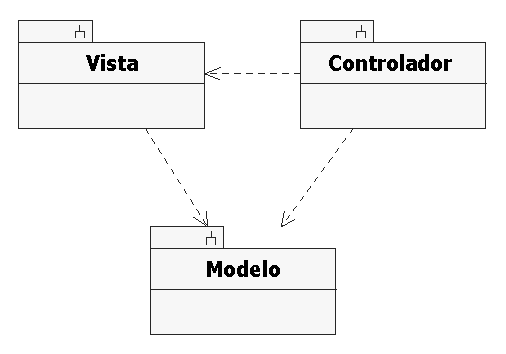
\includegraphics[width=14cm]{diseno/arquitectura/arquitectura_propuesta/diagramas/mvc.eps}
\caption{Patr�n arquitect�nico Modelo-Vista-Controlador}
\end{figure}

\begin{itemize}
\item \textbf{Modelo}
	\begin{itemize}
	\item Contiene la representaci�n y la l�gica de la aplicaci�n.
	\item Se encarga de almacenar y procesar la informaci�n.
	\end{itemize}
\item \textbf{Vista}
	\begin{itemize}
	\item Contiene los mecanismos para mostrar la informaci�n al usuario.
	\item Se encarga de mostrar la informaci�n al usuario de la aplicaci�n.
	\item Depende de Modelo.
	\end{itemize}
\item \textbf{Controlador}
	\begin{itemize}
	\item Contiene los mecanismos para recibir las peticiones del usuario.
	\item Se encarga de atender las peticiones del usuario y entregar dichas peticiones al Modelo o a la Vista.
	\item Depende de Modelo y Vista.
	\end{itemize}
\end{itemize}

El comportamiento t�pico del patr�n MVC suele ser el siguiente:
\begin{enumerate}
\item El usuario utiliza el interfaz del programa para hacer una petici�n al sistema.
\item El Controlador recibe la petici�n.
\item El Controlador env�a al Modelo una o varias peticiones de operaci�n.
\item El Modelo modifica su estado seg�n las peticiones.
\item El Controlador env�a a la Vista una petici�n de actualizaci�n.
\item La Vista recoge la informaci�n necesaria del Modelo.
\item La Vista muestra la informaci�n recogida en el interfaz del programa.
\item El usuario ve el resultado de la operaci�n en el interfaz del programa.
\end{enumerate}

\begin{figure}[]
\centering
\includegraphics[width=14cm]{diseno/arquitectura/arquitectura_propuesta/diagramas/mvc_secuencia.eps}
\caption{Modelo din�mico del patr�n arquitect�nico Modelo-Vista-Controlador}
\end{figure}

Para un videojuego, se necesita que el interfaz del programa se actualice continuamente. Por ello, en este caso el sistema se actualizar� incluso \emph{cuando el jugador no haga nada}, ya que puede que est� esperando a que ocurra alg�n evento del juego. Por ello, la asignaci�n final de responsabilidades del controlador var�a ligeramente. La \emph{no-actuaci�n} del jugador se interpretar� como una forma especial de petici�n.


\section{Dise�o de la arquitectura}
\subsection{Descomposici�n en subsistemas}
Debido a la amplitud del sistema, �ste ha sido descompuesto en un importante n�mero de subsistemas. A continuaci�n se describir�n �stos.

\begin{figure}[]
\centering
\includegraphics[width=14cm]{diseno/arquitectura/arquitectura_propuesta/diagramas/arq_detallada.eps}
\caption{Modelo arquitect�nico detallado}
\end{figure}

\subsubsection{Descomposici�n de Modelo}
Modelo se ha descompuesto en gran cantidad de subsistemas, siguiendo un modelo de \emph{grandes bloques}.
\begin{itemize}
\item \textbf{Motor gr�fico}
	\begin{itemize}
	\item Contiene los modelos de representaci�n gr�fica.
	\item Se encarga de gestionar todo lo que se muestra en pantalla. Esto incluye desde p�xeles sueltos y pol�gonos hasta pantallas o ventanas de aplicaci�n.
	\end{itemize}
\item \textbf{Motor de sonido}
	\begin{itemize}
	\item Contiene los modelos de representaci�n de sonido.
	\item Se encarga de gestionar todo lo que suena por los altavoces o auriculares.
	\end{itemize}
\item \textbf{Motor de procesos}
	\begin{itemize}
	\item Proporciona una base para la implementaci�n de la l�gica del juego.
	\item Se encarga de gestionar la l�gica del juego y de inicializar el juego una vez todos los subsistemas han sido inicializados.
	\end{itemize}
\item \textbf{Bind}
	\begin{itemize}
	\item Proporciona a la l�gica del juego un enlace con las peticiones del jugador.
	\item Se encarga de entregar las �rdenes del jugador a la l�gica del juego.
	\end{itemize}
\item \textbf{L�gica del juego}
	\begin{itemize}
	\item Este subsistema lo debe \emph{rellenar} el desarrollador que utilice el sistema para desarrollar su juego.
	\item Se encarga de procesar el modelo de comportamiento del juego, a partir de la entrada recibida a trav�s de Bind, bas�ndose en el modelo de Procesos y entregando el resultado al Motor de Sonido y al Motor Gr�fico.
	\item Depende de Motor gr�fico, Motor de sonido, Motor de procesos y Bind.
	\end{itemize}
\end{itemize}

\subsubsection{Descomposici�n de Motor gr�fico}
El motor gr�fico es un subsistema complejo, con una gran cantidad de operaciones que tratan desde el control de un p�xel hasta el control de toda la pantalla. Por ello se ha optado en descomponerlo en subsistemas. En este caso se ha utilizado un patr�n Capas. Para la implementaci�n final del mecanismo se ha optado por un patr�n estrategia aplicado a subsistemas. A continuaci�n se describir� cada uno de los subsistemas.

\begin{figure}[]
\centering
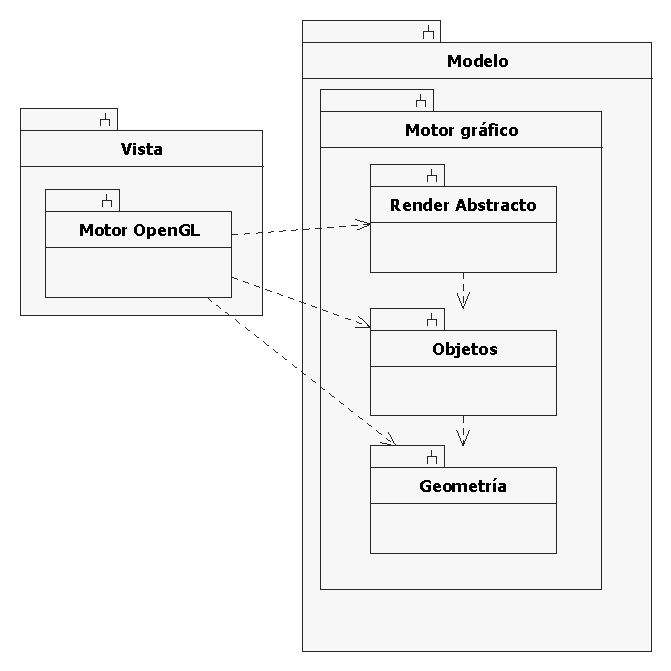
\includegraphics[width=14cm]{diseno/arquitectura/arquitectura_propuesta/diagramas/motor_grafico.eps}
\caption{Diagrama de subsistemas del Motor gr�fico}
\end{figure}

\begin{itemize}
\item \textbf{Geometr�a}
	\begin{itemize}
	\item Se encarga de almacenar y procesar los pol�gonos como unidades individuales.
	\end{itemize}
\item \textbf{Objetos}
	\begin{itemize}
	\item Proporciona un mecanismo para utilizar de una manera l�gica las mallas de pol�gonos.
	\item Se encarga de procesar las mallas como si fueran objetos f�sicos que pudieramos mover con facilidad.
	\item Se encarga de mantener la estructura general de la escena.
	\end{itemize}
\item \textbf{Render abstracto}
	\begin{itemize}
	\item Proporciona mecanismos para manipular la pantalla y c�mo se pintan las escenas.
	\item Se encarga de controlar el uso de la pantalla y los mecanismos para pintar las escenas adecuadamente.
	\end{itemize}
\item \textbf{Motor OpenGL}
	\begin{itemize}
	\item Implementa el motor gr�fico a trav�s de la biblioteca gr�fica OpenGL.
	\item Se encarga de convertir la escena abstracta que haya sido construida utilizando los subsistemas de Geometr�a, Objetos y Render Abstracto en una serie optimizada de llamadas a la biblioteca OpenGL.
	\end{itemize}
\end{itemize}

\subsection{Topolog�a del sistema}
\subsection{Descripci�n de las interfaces}

\subsection{Gesti�n de la persistencia}
Debido al tipo de sistema que se propone, es necesario proveer una estructura b�sica de preparaci�n y recuperaci�n de la informaci�n. Para ello se propone dividir este proceso en dos secciones:
\subsubsection{Preparaci�n y almacenamiento de la informaci�n}
Por una parte es necesario pre-procesar y almacenar los datos necesarios.
\begin{itemize}
\item \textbf{Mallas 3D}
	\begin{itemize}
	\item Las mallas de pol�gonos se crear�n y editar�n con la herramienta Blender.
	\item Una vez completadas las mallas de pol�gonos, se utilizar� dentro de Blender un script que generar� un archivo f�cilmente importable por el sistema.
	\end{itemize}
\item \textbf{Texturas}
	\begin{itemize}
	\item Las texturas para las mallas se generar�n con un programa de retoque fotogr�fico. Se propone por ejemplo The Gimp.
	\item Dichas texturas ser�n exportadas en formatos concretos y con caracter�sticas concretas, para que el sistema pueda importarlas.
	\end{itemize}
\item \textbf{Sonidos}
	\begin{itemize}
	\item Los sonidos ser�n preparados con un programa de edici�n de sonidos. Se propone por ejemplo el programa Audacity.
	\item Dichos sonidos ser�n exportados en formatos concretos para que el sistema pueda importarlos.
	\end{itemize}
\item \textbf{M�sica} \newline
La m�sica es m�s dif�cil de generar que los sonidos. Hay algunos tipos de programa preparados con el fin de crear m�sica. Por ello se propone que la m�sica se prepare en dos pasos
	\begin{itemize}
	\item Se genera con alg�n tipo de programa de creaci�n de m�sica, como puede ser un tracker. Para ello se propone como tracker, el ModPlug Tracker.
	\item La m�sica ser� editada y exportada a un formato de compresi�n con p�rdida de informaci�n, con el fin de evitar generar ficheros demasiado grandes. Para ello se propone el mismo programa que se utiliz� en la fase anterior: Audacity.
	\item El sistema utilizar� un mecanismo especial para importar estos ficheros, evitando cargarlos por completo, ya que pueden ser ficheros grandes.
	\end{itemize}
\end{itemize}

\subsubsection{Recuperaci�n de la informaci�n}
En este sistema se sientan las bases para crear un videojuego, pero no se especifica dicho videojuego. Por ello se debe crear un sistema muy flexible de carga de informaci�n, para que el desarrollador siga manteniendo el control sobre qu� se carga y en qu� momento. 

Por eso se propone un patr�n de f�bricas que lean ficheros e instancien las clases con la informaci�n, siempre a petici�n de los subsistemas del desarrollador.

\subsection{Aspectos globales y de seguridad}
\subsection{Aspectos de rendimiento y tama�o}




%\chapter{Patr�n Observador-Dibujador}
\section{Introducci�n}
El patr�n Observador-Dibujador define una dependencia entre un objeto conceptual y una forma o varias de dibujar dicho objeto, de tal manera que el mecanismo de dibujado del objeto est� desacoplado del objeto, y pueda cambiar sin que el objeto tenga que enterarse.
\subsection{Motivo}
El patr�n Observador-Dibujador tiene dos partes que son el Objeto y el Dibujador. Uniendo estas dos partes hay una mara�a de clases que a�aden funcionalidad para poder cambiar el Dibujador din�micamente.

Un ejemplo de uso de este patr�n es en el mecanismo de dibujado de una malla poligonal en pantalla, de tal manera que queda separado el modelo conceptual de malla del mecanismo que se utiliza para dibujar dicha malla en pantalla.
\subsection{Aplicabilidad}
Se puede usar el patr�n Observador-Dibujador en las siguientes situaciones:
\begin{itemize}
\item Cuando en un patr�n observador el sujeto desconoce c�mo debe ser tratado, o si su manera de ser tratado cambiar� en cualquier momento.
\end{itemize}
\subsection{Consecuencias}
\begin{itemize}
\item La fuerte separaci�n entre el sujeto y el observador-dibujador garantiza que es f�cil reaprovechar el sujeto.
\item Es sencillo cambiar radicalmente de mecanismo de dibujado cambiando din�micamente el observador-dibujador.
\end{itemize}
\subsection{Usos conocidos}
\subsection{Patrones relacionados}
\section{Estructura de clases}
\subsection{Colaboraciones}
\subsection{Detalles de implementaci�n}
\section{Descripci�n de las clases}
\section{Ejemplo de uso}
\section{Referencias}

%\chapter{Dise�o del subsistema Geometr�a}
En esta secci�n se trata el subsistema Geometr�a. Este subsistema ha sido propuesto como una estructura de datos pensada para almacenar geometr�a. 

Con el fin de permitir que el sistema sea extendido m�s adelante, pero manteniendo las estructuras b�sicas, cada clase de an�lisis ha sido dividida en una abstracta y una concreta. En este caso la concreta implementa el modelo m�s sencillo de malla.

Adem�s, ha sido a�adido el mecanismo para cargar mallas, a trav�s de una f�brica abstracta.

\section{Vista de casos de uso}
A pesar de que ning�n caso de uso de an�lisis afecta directamente a este subsistema, se hace necesario documentar los mecanismos de carga de mallas y dibujado de las mismas.
\subsection{Carga de mallas}
Este caso de uso implementa la carga de una malla de pol�gonos. En este caso concreto se indica la carga de una malla simple mediante la f�brica correspondiente. A continuaci�n se especifica el flujo de eventos.

%------------------------------------------- Copypaste
\renewcommand{\labelenumi}{%
 \textbf{\theenumi}.-
}

\renewcommand{\theenumii}{\arabic{enumii}}
\renewcommand{\labelenumii}{%
 \textbf{\theenumi}.\theenumii.-
}

\renewcommand{\theenumiii}{\arabic{enumiii}}
\renewcommand{\labelenumiii}{%
 \textbf{\theenumi}.\theenumii.\theenumiii.-
}

%-----------------------------------------------------
\begin{enumerate}
\item El cliente prepara fichero:Dispositivo\_entrada\_caracteres.
\item El cliente llama f�brica.cargar\_malla(fichero), siendo f�brica:Cargador\_malla.
\item F�brica procesa la llamada y procede a cargar el fichero.
	\begin{enumerate}
	\item Para cada coordenada, normal, color y uv del fichero:
		\begin{enumerate}
		\item Carga el dato
		\item Instancia el elemento
		\end{enumerate}
	\item Para cada v�rtice del fichero:
		\begin{enumerate}
		\item Carga informaci�n del v�rtice
		\item Prepara asociaciones del v�rtice
		\item Instancia el v�rtice
		\end{enumerate}
	\item Para cada material del fichero:
		\begin{enumerate}
		\item Carga informaci�n del material
		\item Instancia el material
		\item Instancia una capa
		\item Enlaza la capa al material
		\end{enumerate}
	\item Para cada pol�gono del fichero:
		\begin{enumerate}
		\item Carga informaci�n del pol�gono
		\item Prepara asociaciones del pol�gono
		\item Instancia el pol�gono
		\end{enumerate}
	\item Prepara asociaciones de la malla
	\item Instancia la malla
	\end{enumerate}
\item F�brica devuelve la malla instanciada.
\end{enumerate}

Como se puede apreciar, el proceso de carga no es trivial, pero es sencillo de comprender. B�sicamente, F�brica se encarga de cargar la malla e instanciar todos los objetos.

\subsection{Mecanismo de dibujado}
El mecanismo de dibujado de mallas es complejo, ya que se pretende que sea desacoplable del mecanismo concreto. Por ello se propone utilizar el patr�n observador. Este patr�n se encargar� de llevar los cambios que se produzcan en el motor gr�fico al motor concreto de pintado.

Por ello, todas las clases significativas de ser pintadas en pantalla o de influenciar lo que se pinte en pantalla ser�n \emph{sujetos} en el patr�n.

Inicialmente no se propone un mecanismo de pintado concreto. Sin embargo, es evidente que es necesario pintar la escena en pantalla, y por eso se implementar� un ejemplo de motor en OpenGL, que es donde se alojar�n algunas de las clases \emph{observador} del patr�n.

El mecanismo final de pintado de mallas ser� por tanto un mecanismo doble. Por una parte est� el modelo abstracto de geometr�a, definido por las clases que se encuentran en el motor gr�fico. Y por otra parte est� el modelo optimizado al mecanismo concreto de pintado, definido por las clases en el motor concreto de pintado, en este caso Motor OpenGL. Este �ltimo modelo ser� el que realmente se pinte en pantalla, y ser� guiado y actualizado por el modelo abstracto a trav�s del patr�n observador.




\section{Vista l�gica}
Debido a que es posible que algunas mallas no se dibujen en pantalla (se utilicen para detecci�n de colisiones, por ejemplo) y a que puede ser interesante desarrollar m�s tipos de malla m�s adelante, se hace necesario \emph{llevar la cuenta} de las mallas que se vayan a dibujar y su tipo. Esto hace aparecer algunas clases \emph{contador}, que no son m�s que agregadores bajo el estereotipo <<singleton>>.

Se ha optado por separar las clases en una abstracci�n y una implementaci�n. Esto se hace con el fin de facilitar la creaci�n de nuevos tipos de malla, y su posterior utilizaci�n por parte de la l�gica del juego. Por otra parte, se propone a la hora de crear nuevos tipos de malla que se utilice herencia a partir de la abstracci�n, especificando a partir de la clase origen \emph{y} de sus relaciones. A efectos pr�cticos, la abstracci�n se utiliza como una interfaz.

A continuaci�n se describir�n las clases principales del sistema.

\subsection{Malla}
Almacena una malla de pol�gonos.
\begin{itemize}
\item \textbf{Responsabilidades:}
	\begin{itemize}
	\item Almacenar una malla de pol�gonos.
	\end{itemize}
\item \textbf{Relaciones:}
	\begin{itemize}
	\item -pol�gonos : colecci�n de pol�gono \newline
		Los pol�gonos de la malla.
	\end{itemize}
\item \textbf{M�todos:}
	\begin{itemize}
	\item +pol�gonos() : colecci�n de pol�gono \newline
		Los pol�gonos de la malla.
	\end{itemize}
\end{itemize}

\subsection{Malla\_simple}
Representa una malla de pol�gonos sencilla. No tiene animaci�n, ni controles externos. Es el modelo de malla con materiales, capas y texturas m�s sencillo.
\begin{itemize}
\item \textbf{Responsabilidades:}
	\begin{itemize}
	\item Almacenar una malla de pol�gonos.
	\end{itemize}
\item \textbf{Relaciones:}
	\begin{itemize}
	\item -pol�gonos : colecci�n de pol�gono \newline
		Los pol�gonos de la malla.
	\item Es una especificaci�n de Malla. Implementa por tanto una variante de Malla.
	\end{itemize}
\item \textbf{M�todos:}
	\begin{itemize}
	\item +pol�gonos() : colecci�n de pol�gono \newline
		Los pol�gonos de la malla.
	\end{itemize}
\end{itemize}

\subsection{Cargador\_malla}
Provee un interfaz para crear una f�brica de mallas.
\begin{itemize}
\item \textbf{Responsabilidades:}
	\begin{itemize}
	\item Cargar e instanciar una malla.
	\end{itemize}
\item \textbf{Relaciones:}
	\begin{itemize}
	\item <<access>> Dispositivo\_entrada\_caracteres \newline
		Lee la informaci�n de la malla del dispositivo entregado.
	\item <<instantiate>> Malla. \newline
		Instancia mallas.
	\end{itemize}
\item \textbf{M�todos:}
	\begin{itemize}
	\item +\emph{cargar}(d : Dispositivo\_entrada\_caracteres) : malla \newline
		Carga una malla desde el dispositivo indicado. Falla si el dispositivo no contiene la informaci�n de la malla en el formato correcto.
	\end{itemize}
\end{itemize}

\subsection{Cargador\_malla\_simple}
Se encarga de cargar e instanciar Malla\_simple
\begin{itemize}
\item \textbf{Responsabilidades:}
	\begin{itemize}
	\item Leer la informaci�n de una Malla\_simple e instanciarla.
	\end{itemize}
\item \textbf{Relaciones:}
	\begin{itemize}
	\item <<instantiate>> Malla\_simple. \newline
		Instancia Malla\_simple.
	\end{itemize}
\item \textbf{M�todos:}
	\begin{itemize}
	\item +cargar(d : Dispositivo\_entrada\_caracteres) : malla \newline
		Llama a cargar\_malla\_simple.
	\item +cargar\_malla\_simple(d : Dispositivo\_entrada\_caracteres) : Malla\_simple \newline
		Carga e instancia una Malla\_simple desde el dispositivo de entrada indicado. No se ha especificado, pero este m�todo puede ser muy complicado, incluyendo un lexer y un parser con el fin de leer ficheros y comprobar que es correcta la sintaxis.
	\end{itemize}
\end{itemize}





%\chapter{Dise�o del subsistema Objetos}

\section{Vista de casos de uso}

\section{Vista l�gica}

%\chapter{Dise�o del subsistema Render abstracto}

\section{Vista de casos de uso}

\section{Vista l�gica}

%\chapter{Dise�o del subsistema Motor OpenGL}

\section{Vista de casos de uso}
\section{Vista l�gica}

%\chapter{Introducci�n}
Hasta ahora se ha especificado en general c�mo debe ser la forma y el comportamiento de las clases y del sistema. En este punto se discutir� al detalle c�mo debe ser implementado el sistema. Por ello, hasta este punto se ha estado hablando en t�rminos abstractos, en el c�mo deber�a funcionar. En este punto se especificar�n los mecanismos y detalles concretos que llevar� la implementaci�n.

\section{Restricciones y conversiones}
Para implementar este proyecto se utilizar� el lenguaje OCaML, que al igual que cualquier otro lenguaje de programaci�n tiene sus particularidades. Por ello, a continuaci�n se especifica una peque�a gu�a para transformar los modelos de an�lisis y dise�o a este lenguaje.

\begin{itemize}
\item \textbf{Tipos de dato}
	\begin{itemize}
	\item Void o vac�o, el tipo de dato que especifica que no se pasa nada de par�metro o no se devuelve nada, pasa a llamarse \emph{unit}.
	\item Conjunto ordenado, el tipo de dato que especifica una relaci�n con varias unidades siguiendo un determinado orden, pasa a ser \emph{array} o \emph{list}, dependiendo si es necesario el acceso r�pido a un elemento concreto o la capacidad de recorrer todos los elementos en orden.
	\item Conjunto, el tipo de dato que especifica una relaci�n con varias unidades, pasa a llamarse \emph{list}, por la facilidad de a�adir o filtrar elementos.
	\item Vector, Vector4, Vector3 y Vector2 son la misma clase con distintos nombres. La �nica diferencia reside en que si a Vector4, Vector3 o Vector2 se le pasa una cantidad de par�metros distinto al n�mero de la clase, se quejan y fallan con una excepci�n. Esto se hace con el fin de favorecer los controles de precondici�n y postcondici�n.
	\end{itemize}
\item \textbf{Operaciones del lenguaje}
	\begin{itemize}
	\item OCaML es un lenguaje fuertemente tipado, con inferencia de tipos. Debido a estas caracter�sticas, no es posible hacer \emph{downcasting}, es decir, transformar una referencia a una clase en una referencia a una de sus subclases. Esto se considera una operaci�n peligrosa y ambigua, y esa es la raz�n de que el lenguaje se niegue a implementarla.
	\item Debido a que el \emph{downcasting} es imposible, el \emph{upcasting} es una operaci�n de una s�la direcci�n, y no se puede invertir. Hay que crear caminos alternativos donde el \emph{downcasting} ser�a necesario.
	\item OCaML pone muchas trabas a la hora de crear dependencias circulares. Esto ha favorecido la creaci�n de un modelo de an�lisis y dise�o libre de dependencias circulares.
	\end{itemize}
\end{itemize}

\chapter{Dise�o detallado de las clases}

\section{Cargador\_malla\_simple}
Se encarga de cargar e instanciar Malla\_simple. Incluye un lexer y un parser que se encargan de la lectura del fichero. Tanto el lexer como el parser se har�n con herramientas ya disponibles: OcamlLex y OcamlYACC.

OcamlLex y OcamlYACC generan cada uno un m�dulo nuevo que es utilizado por Cargador\_malla\_simple. Estos m�dulos se llaman \emph{Cargador\_malla\_lexer} y \emph{Cargador\_malla\_parser}.

\begin{itemize}
\item \textbf{Relaciones:}
	\begin{itemize}
	\item <<instantiate>> Clases del tipo *\_simple. \newline
		Instancia Malla\_simple y las clases que utilice Malla\_simple. Adem�s, realiza la interconexi�n de estas clases.
	\item <<uso>> Utiliza una instancia de Dispositivo\_entrada\_caracteres para leer el fichero.
	\end{itemize}
\item \textbf{M�todos:}
	\begin{itemize}
	\item +cargar(d : Dispositivo\_entrada\_caracteres) : malla \newline
		Llama a cargar\_malla\_simple. Devuelve el resultado como malla, y no malla\_simple, con el fin de utilizarlo para alg�n tipo de cargador abstracto.
	\item +cargar\_malla\_simple(d : Dispositivo\_entrada\_caracteres) : Malla\_simple \newline
		Carga e instancia una Malla\_simple desde el dispositivo de entrada indicado.
	\end{itemize}
\end{itemize}

\subsection{El lexer}
El lexer se encarga de leer los caracteres del fichero y transformarlos en elementos de prean�lisis para el parser. A continuaci�n se describen estos elementos.

\newcommand{\elemento}[2]{\item \textbf{#1} \newline #2}
\begin{itemize}
\elemento{\emph{espacio en blanco}}{Ignorado}
\elemento{\emph{tabulador}}{Ignorado}
\elemento{\emph{retorno de carro}}{Ignorado}
\elemento{\#, \emph{cualquier caracter excepto retorno de carro}, \emph{retorno de carro}}{Ignorado, es un comentario}
\elemento{\emph{n�mero real}}{REAL}
\elemento{\emph{n�mero entero}}{ENTERO}
\elemento{", \emph{cadena de caracteres}, "}{CADENA}
\elemento{version}{VERSION}
\elemento{o}{OBJETO}
\elemento{nv}{NUMVERTICES}
\elemento{v}{VERTICE}
\elemento{nm}{NUMMATERIALES}
\elemento{m}{MATERIAL}
\elemento{tex}{TEXTURA}
\elemento{notex}{NOTEXTURA}
\elemento{esp}{ESPECULAR}
\elemento{emi}{EMISION}
\elemento{nf}{NUMCARAS}
\elemento{f}{CARA}
\elemento{fm}{MATERIAL\_CARA}
\elemento{fv}{VERTICE\_CARA}
\elemento{fvuc}{VERTICE\_CARA\_UV\_COLOR}
\elemento{\emph{fin de fichero}}{EOF}
\end{itemize}

\subsection{El parser}
El parser se encarga de procesar los elementos de prean�lisis del lexer, comprobar que siguen la sintaxis especificada y construir la malla a partir de la informaci�n del fichero. A continuaci�n se especifican las reglas del parser.

En may�sculas, los terminales definidos en la secci�n anterior. En min�sculas, los auxiliares. Cada palabra es un \emph{s�mbolo}. 

S�mbolo inicial: main\newline
\newcommand{\regla}[2]{\item\textbf{#1} -\textgreater \newline #2}
\begin{itemize}
\regla{main}{version nombre vertices materiales caras EOF}
\regla{version}{VERSION REAL}
\regla{nombre}{OBJETO CADENA}
\regla{vertices}{NUMVERTICES ENTERO desc\_vertices}
\regla{desc\_vertices}{desc\_vertice desc\_vertices \newline \textbar desc\_vertice}
\regla{desc\_vertice}{VERTICE REAL REAL REAL REAL REAL REAL}
\regla{materiales}{NUMMATERIALES ENTERO desc\_materiales}
\regla{desc\_materiales}{desc\_material desc\_materiales \newline \textbar desc\_material}
\regla{desc\_material}{MATERIAL CADENA textura difuso especular emision}
\regla{textura}{TEXTURA CADENA \newline \textbar NOTEXTURA}
\regla{difuso}{DIFUSO REAL REAL REAL REAL}
\regla{especular}{ESPECULAR REAL REAL REAL REAL REAL}
\regla{emisi�n}{EMISION REAL REAL REAL REAL}
\regla{caras}{NUMCARAS ENTERO desc\_caras}
\regla{desc\_caras}{desc\_cara desc\_caras \newline \textbar desc\_cara}
\regla{desc\_cara}{CARA material\_cara vertices\_cara}
\regla{material\_cara}{MATERIAL\_CARA ENTERO}
\regla{vertices\_cara}{vertice\_cara vertice\_cara vertice\_cara \newline \textbar vertice\_cara vertice\_cara vertice\_cara vertice\_cara}
\regla{vertice\_cara}{VERTICE\_CARA ENTERO \newline \textbar VERTICE\_CARA\_UV\_COLOR ENTERO REAL REAL REAL REAL REAL REAL}
\end{itemize}





%\part{Modelo de implementaci�n}
%\input{implementacion/implementacion.tex}
%%\subsubsection{Relaciones}
%\begin{itemize}
%\end{itemize}
%\subsubsection{Atributos}
%\begin{itemize}
%\end{itemize}
%\subsubsection{M�todos}
%\begin{itemize}
%\item +inicializador \newline
%\end{itemize}
%\subsubsection{Par�metros de instanciaci�n}
%\begin{itemize}
%\end{itemize}


\chapter{Clases generales}
En este cap�tulo se describen algunas clases de uso general que se utilizan en el sistema.

\section{Patr�n observador}
Estas clases son las clases generales de uso con el patr�n observador.
\subsection{\emph{observador}}
Implementa un observador abstracto.
\subsubsection{M�todos}
\begin{itemize}
\item +actualizar \newline
Ordena la actualizaci�n del estado del Observador.
\end{itemize}

\subsection{\emph{sujeto}}
\subsubsection{Relaciones}
\begin{itemize}
\item Depende de \Clase{Observador}.
\end{itemize}
\subsubsection{Atributos}
\begin{itemize}
\item observadores : \Clase{Observador} list \newline
Los observadores que est�n observando al sujeto en concreto.
\end{itemize}
\subsubsection{M�todos}
\begin{itemize}
\item +observadores : \Clase{Observador} list \newline
Los observadores que est�n observando al sujeto en concreto.
\item +a�adir\_observador (o:\Clase{observador}) \newline
Pone un nuevo observador en la lista de observadores.
\item +eliminar\_observador (o:\Clase{observador}) \newline
Quita un observador de la lista de observadores.
\item +notificar \newline
Llama al m�todo \emph{actualizar} para cada observador en la lista de observadores.
\end{itemize}

\section{Agregadores}
Clases que act�an como agregadores con caracter�sticas especiales.

\subsection{agregador}
Un agregador gen�rico y parametrizado. 't es el tipo del objeto agregado para una instancia concreta de \Clase{agregador}.
\subsubsection{Atributos}
\begin{itemize}
\item contenido : \emph{Conjunto vac�o} \newline
Los objetos, agregados mediante el m�dulo Conjunto.
\end{itemize}
\subsubsection{M�todos}
\begin{itemize}
\item +agregar (x:'t) \newline
Agrega el objeto.
\item +quitar (x:'t) \newline
Quita el objeto.
\item +pertenece (x:'t) : bool \newline
Comprueba si el objeto ya est� agregado al agregador.
\item +obtener\_todos : 't list \newline
Devuelve una lista con todos los objetos del agregador.
\end{itemize}

\subsection{agregador\_observado}
Es un \Clase{agregador} que adem�s es un \Clase{sujeto} dentro del patr�n observador. Notifica a sus \Clase{Observadores} cuando agrega o quita un elemento. El tipo del objeto agregado es 't.
\subsubsection{Relaciones}
\begin{itemize}
\item Es una especificaci�n de 't \Clase{agregador} (un \Clase{Agregador} de objetos de tipo 't).
\item Es una especificaci�n de sujeto.
\end{itemize}
\subsubsection{Atributos}
\begin{itemize}
\item ultima\_accion : t\_ultima\_accion option \newline
Almacena la �ltima operaci�n que hizo el agregador, ya sea agregar o quitar.
\end{itemize}
\subsubsection{M�todos}
\begin{itemize}
\item +ultima\_accion : t\_ultima\_accion \newline
Devuelve la �ltima operaci�n del agregador, o falla si no hubo �ltima.
\item +agregar (x:'t) \newline
Agrega un objeto, guarda \emph{Agregar} como �ltima acci�n y notifica a sus observadores.
\item +quitar (x:'t) \newline
Desagrega un objeto, guarda \emph{Quitar} como �ltima acci�n y notifica a sus observadores.
\end{itemize}

\subsection{asociador}
Asocia objetos de tipo 'a a objetos de tipo 'b, de tal manera que cada objeto de tipo 'a dentro del asociador tiene un objeto de tipo 'b.
\subsubsection{Atributos}
\begin{itemize}
\item contenido : \emph{Asociador vac�o} \newline
Las parejas de objetos, asociadas mediante el m�dulo Asociador.
\end{itemize}
\subsubsection{M�todos}
\begin{itemize}
\item +asociar (a:'a) (b:'b) \newline
Asocia al objeto a con el objeto b.
\item +quitar\_asociaci�n (a:'a) \newline
Elimina dentro del asociador la relaci�n entre el objeto a y su asociado.
\item +buscar\_asociado (a:'a) : 'b \newline
Busca el objeto asociado al objeto a. Falla si no hay ninguno.
\end{itemize}


\section{Ficheros}
Estas clases se refieren a ficheros y mecanismos similares.
\subsection{\emph{dispositivo\_entrada\_caracteres}}
Clase abstracta que provee el interfaz para acceder a un dispositivo de lectura del que se pueden leer caracteres. Al leer todos los m�todos avanzan el puntero de lectura y lanzan una excepci�n \emph{End\_of\_file} si se intenta leer m�s all� de los l�mites del fichero.
\subsubsection{M�todos}
\begin{itemize}
\item +leer\_caracter : char \newline
Lee un caracter y avanza el puntero de lectura.
\item +leer\_linea : string \newline
Lee hasta encontrar un retorno de carro.
\item +leer\_cadena (n:int) : (int * string) \newline
Intenta leer n caracteres. Devuelve la cadena le�da y el n�mero de caracteres le�dos. Si llega al final del fichero antes de leer n caracteres devuelve la cantidad le�da sin lanzar ninguna excepci�n.
\item +leer\_cadena\_completa (n:int) : string \newline
Lee n caracteres. Si no hay caracteres suficientes lanza la excepci�n \emph{End\_of\_file}.
\item +longitud : int \newline
La longitud completa del fichero.
\item +posici�n\_lectura : int \newline
La posici�n del puntero de lectura.
\item +set\_posicion\_lectura (n:int) \newline
Cambia la posici�n del puntero de lectura.
\end{itemize}

\subsection{fichero\_entrada}
Implementa la lectura de un fichero de disco.

\subsubsection{Relaciones}
\begin{itemize}
\item Es una especificaci�n de \Clase{Dispositivo entrada caracteres}
\end{itemize}
\subsubsection{Atributos}
\begin{itemize}
\item archivo : in\_channel \newline
El manejador del archivo.
\end{itemize}
\subsubsection{Par�metros de instanciaci�n}
\begin{itemize}
\item fn : string \newline
La ruta del fichero en disco.
\end{itemize}

\section{Matem�ticas}
\subsection{vector}
\subsubsection{Relaciones}
\begin{itemize}
\item Depende de \Clase{Matriz}.
\end{itemize}
\subsubsection{Atributos}
\begin{itemize}
\item vector : float array \newline
Un array con el contenido del vector.
\end{itemize}
\subsubsection{M�todos}
\begin{itemize}
\item +to\_list : float list \newline
El contenido del vector como lista.
\item +to\_array : float array \newline
El contenido del vector como array.
\item +num\_elementos : int \newline
El n�mero de elementos o dimensi�n del vector.
\item +dimensi�n : int \newline
Lo mismo que num\_elementos.
\item +elemento (i:int) : float \newline
El elemento i-�simo del vector, empezando por 1.
\item +suma (v2:vector) : vector \newline
Suma dos vectores elemento a elemento. Tienen que tener la misma cantidad de elementos.
\item +producto\_escalar (e:float) : vector \newline
Devuelve un vector de tal manera que es el resultado de multiplicar cada elemento del vector actual por e.
\item +producto\_interior (b:vector) : float \newline
Siendo los vectores a y b devuelve
\begin{math}
\sum_{} a_{i} b_{i}
\end{math}
\item +longitud : float \newline
Siendo a el vector devuelve
\begin{math}
\sqrt{\sum_{} a_{i}^2}
\end{math}
\item +a\_unitario : vector \newline
Escala el vector hasta que su longitud es 1.
\item +a\_fila : matriz \newline
Convierte el vector en una matriz fila.
\item +a\_columna : matriz \newline
Convierte el vector en una matriz columna.
\item +fila\_por\_matriz (m:matriz) : vector \newline
Multiplica el vector como fila por la matriz.
\item +producto\_cruzado (b:vector) : vector \newline
Realiza el producto cruzado, tambi�n llamado producto vectorial o producto externo, de dos vectores ambos de 2 o 3 dimensiones.
\item +a\_string : string \newline
Devuelve una cadena de texto con el contenido del vector en un formato f�cilmente legible por personas.
\end{itemize}
\subsubsection{Par�metros de instanciaci�n}
\begin{itemize}
\item v : float array \newline
Un array con los elementos que contendr� el vector.
\end{itemize}

\subsection{vector2}
Un alias para \Clase{vector}, pero garantiza que ser� un vector de dimensi�n 2.

\subsection{vector3}
Un alias para \Clase{vector}, pero garantiza que ser� un vector de dimensi�n 3.

\subsection{vector4}
Un alias para \Clase{vector}, pero garantiza que ser� un vector de dimensi�n 4.


\subsection{matriz}
\subsubsection{Relaciones}
\begin{itemize}
\item Depende de \Clase{vector}.
\end{itemize}
\subsubsection{Atributos}
\begin{itemize}
\item mat : float array array \newline
Contiene la matriz como un array de arrays.
\end{itemize}
\subsubsection{M�todos}
\begin{itemize}
\item +num\_filas : int \newline
El n�mero de filas de la matriz.
\item +num\_columnas : int \newline
El n�mero de columas de la matriz.
\item +extrae\_fila (i:int) : vector \newline
Extrae la fila i-�sima de la matriz, empezando por 1.
\item +extrae\_columna (j:int) : vector \newline
Extrae la columna j-�sima de la matriz, empezando por 1.
\item +extrae\_elemento (i:int) (j:int) : float \newline
Siendo M la matriz extrae el elemento 
\begin{math}
M_{ij}
\end{math}.
\item +extrae\_submatriz (i1:int, i2:int) (j1:int, j2:int) : matriz \newline
Extrae la submatriz compuesta por las filas desde i1 hasta i2 (ambos inclu�dos) y columnas desde j1 hasta j2 (ambos inclu�dos), empezando la cuenta de filas y columnas por 1.
\item +matriz\_por\_matriz (m2:matriz) : matriz \newline
Devuelve el producto de las dos matrices.
\item +matriz\_por\_columna (v:vector) : vector \newline
Multiplica la matriz por el vector como columna y devuelve el resultado.
\item +traspuesta : matriz \newline
Transpone la matriz.
\item +cambia\_elemento (i:int) (j:int) (nv:float) \newline
Cambia el elemento $M_{ij}$ por nv.
\item +duplica : matriz \newline
Devuelve una copia de la matriz.
\item +a\_string : string \newline
Devuelve la matriz como una cadena de texto legible por una persona.
\end{itemize}
\subsubsection{Par�metros de instanciaci�n}
\begin{itemize}
\item m : float array array \newline
Un array de arrays los elementos que contendr� la matriz.
\end{itemize}

\subsection{cuaternion}
\subsubsection{Relaciones}
\begin{itemize}
\item Depende de \Clase{vector}.
\item Depende de \Clase{Matriz}.
\end{itemize}
\subsubsection{Atributos}
\begin{itemize}
\item a1 : float \newline
La parte real del cuaterni�n.
\item a2 : float
\item a3 : float
\item a4 : float \newline
(a2, a3, a4) conforman la parte imaginaria del cuaterni�n.
\end{itemize}
\subsubsection{M�todos}
\begin{itemize}
\item +valor : (float * float * float * float) \newline
El contenido del cuaterni�n como (a1, a2, a3, a4).
\item +suma (c2:cuaternion) : cuaternion \newline
Suma dos cuaterniones, elemento a elemento.
\item +conjugado : cuaternion \newline
El conjugado del cuaterni�n, es decir, otro cuaterni�n en el que la parte imaginaria ha sido cambiada de signo.
\item +producto (c2:cuaternion) : cuaternion \newline
Siendo c1 y c2 los cuaterniones, devuelve c1 � c2. El producto de dos cuaterniones es asociativo, pero no conmutativo.
\item +longitud : float \newline
Devuelve $\sqrt{\sum a_{i}}$.
\item +a\_unitario : cuaternion \newline
Escala el cuaterni�n hasta que su longitud sea 1.
\item +extrae\_rotacion : (vector * float) \newline
Para un cuaterni�n que expresa una rotaci�n, devuelve dicha rotaci�n como un vector alrededor del que se rota y el �ngulo que se rota, en radianes.
\item +extrae\_vector : vector \newline
Para un cuaterni�n que expresa un vector, devuelve el vector.
\item +a\_matriz\_rotacion : matriz \newline
Convierte un cuaterni�n que expresa una rotaci�n en una matriz de rotaci�n.
\item +to\_string : string \newline
Devuelve una cadena de texto con el cuaterni�n en forma legible.
\end{itemize}
\subsubsection{Par�metros de instanciaci�n}
\begin{itemize}
\item a1 : float\newline
El t�rmino real del cuaterni�n.
\item v : (float * float * float) \newline
El t�rmino imaginario del cuaterni�n.
\end{itemize}

\section{Procesos}
\subsection{\emph{sistema}}
\subsubsection{Relaciones}
\begin{itemize}
\item Depende de \Clase{proceso}.
\end{itemize}
\subsubsection{M�todos}
\begin{itemize}
\item +ejecutar\_procesos \newline
Da una r�faga de CPU a todos los procesos normales.
\item +ejecutar\_dormidos \newline
Da una r�faga de CPU a los procesos dormidos.
\item +a�adir\_proceso (p:proceso) \newline
A�ade un proceso al sistema de procesos.
\end{itemize}

\subsection{\emph{prioridad}}
\subsubsection{Relaciones}
\begin{itemize}
\item Depende de \Clase{Proceso}.
\end{itemize}
\subsubsection{M�todos}
\begin{itemize}
\item +valor : int \newline
El n�mero de prioridad.
\item +ejecutar\_procesos \newline
Da una r�faga de CPU a los procesos normales que tenga asignada esta prioridad.
\item +ejecutar\_dormidos \newline
Da una r�faga de CPU a los procesos dormidos que tenga asignada esta prioridad.
\item +a�adir\_proceso (p:proceso) \newline
A�ade un proceso al sistema de procesos.
\item +eliminar\_proceso (p:proceso) \newline
Elimina un proceso del sistema de procesos.
\item \#pre\_proceso \newline
Es llamado antes de que cualquier prioridad empiece a ejecutar procesos.
\item \#post\_proceso \newline
Es llamado despu�s de que las prioridades hayan ejecutado todos los procesos.
\end{itemize}

\subsection{\emph{proceso}}
\subsubsection{Relaciones}
\begin{itemize}
\item Depende de \Clase{prioridad}.
\end{itemize}
\subsubsection{M�todos}
\begin{itemize}
\item +estado : t\_estado \newline
Devuelve el estado del proceso como \emph{Normal}, \emph{Dormido}, \emph{Congelado}, \emph{Muerto}.
\item +prioridad : int \newline
El valor de prioridad del proceso.
\item +set\_prioridad (i:int) \newline
Cambia la prioridad del proceso.
\item +ejecutar \newline
M�todo al que se llama para dar una r�faga de CPU al proceso.
\item +ejecutar\_dormido \newline
M�todo al que se llama para dar una r�faga de CPU al proceso si est� dormido.
\item +se�al (s:t\_se�al) \newline
Env�a una se�al al proceso, ya sea \emph{Despertar}, \emph{Dormir}, \emph{Congelar} o \emph{Matar}.
\item +evento\_despertar
\item +evento\_dormir
\item +evento\_congelar
\item +evento\_matar
Estos m�todos son llamados cuando el proceso recibe una se�al.
\item +lanzar (p:proceso) \newline
Mete un nuevo proceso en el sistema de procesos.
\end{itemize}

\subsection{prioridad\_impl}
\subsubsection{Relaciones}
\begin{itemize}
\item Es una especificaci�n de \Clase{prioridad}.
\item Depende de \Clase{proceso}.
\item Depende de \Clase{sistema}.
\end{itemize}
\subsubsection{Atributos}
\begin{itemize}
\item normales : proceso list
\item dormidos : proceso list
\item congelados : proceso list
Almacena los procesos seg�n el tipo en esta prioridad.
\item normales\_modificados : proceso list
\item dormidos\_modificados : proceso list
\item congelados\_modificados : proceso list
Almacena los procesos seg�n el tipo mientras cambian durante la r�faga de CPU actual.
\item prioridad : int \newline
Almacena el valor de prioridad.
\end{itemize}

\subsection{sistema\_impl}
\subsubsection{Relaciones}
\begin{itemize}
\item Es una especificaci�n de \Clase{sistema}.
\item Depende de \Clase{prioridad}.
\item Instancia \Clase{prioridad impl}.
\item Depende de \Clase{proceso}.
\end{itemize}
\subsubsection{Atributos}
\begin{itemize}
\item prioridades : prioridad list\newline
Guarda las prioridades del sistema ordenadas por valor.
\end{itemize}
\subsubsection{M�todos}
\begin{itemize}
\item -pre\_proceso \newline
Lanza el m�todo pre\_proceso para cada prioridad.
\item -post\_proceso \newline
Lanza el m�todo post\_proceso para cada prioridad.
\end{itemize}

\subsection{\emph{proceso\_abstract}}
\subsubsection{Relaciones}
\begin{itemize}
\item Es una especificaci�n de \Clase{proceso}.
\item Depende de \Clase{prioridad}.
\end{itemize}
%\subsubsection{Atributos}
%\begin{itemize}
%\end{itemize}
%\subsubsection{M�todos}
%\begin{itemize}
%\end{itemize}

\section{Recursos}
Las siguientes clases organizan la instanciaci�n y destrucci�n de objetos cuyo coste de instanciaci�n sea muy alto (por ejemplo, objetos grandes cargados de disco).
\subsection{\emph{cargador}}
Organiza la carga o descarga de un recurso. El tipo de recurso cargado es 't.
%\subsubsection{Relaciones}
%\begin{itemize}
%\end{itemize}
\subsubsection{Atributos}
\begin{itemize}
\item estado : t\_estado \newline
El estado de carga del recurso. Los estados disponibles son \emph{No\_cargado}, \emph{Carga\_incompleta(porcentaje)}, \emph{Cargado}, \emph{Descarga\_incompleta}, \emph{Error\_carga(descripci�n)}, \emph{Error\_descarga(descripci�n)}.
\end{itemize}
\subsubsection{M�todos}
\begin{itemize}
\item +estado : t\_estado \newline
El estado de carga del recurso.
\item \#cambia\_estado (n:t\_estado) \newline
Cambia el estado de carga.
\item +\emph{cargar} \newline
Comienza la carga del recurso.
\item +\emph{descargar} \newline
Comienza la descarga del recurso.
\item +\emph{obtener} : 't \newline
Devuelve el recurso cargado.
\item +\emph{clonar} : 't \newline
Para un recurso ya cargado, devuelve una copia del recurso.
\end{itemize}

\subsection{\emph{a\_instanciador}}
Instancia objetos de tipo 't.
%\subsubsection{Relaciones}
%\begin{itemize}
%\end{itemize}
%\subsubsection{Atributos}
%\begin{itemize}
%\end{itemize}
\subsubsection{M�todos}
\begin{itemize}
\item +\emph{cargar} \newline
Carga el recurso asociado al objeto.
\item +\emph{descargar} \newline
Descarga el recurso asociado al objeto.
\item +\emph{obtener} : 't \newline
Instancia el objeto.
\item +\emph{obtener\_duplicado} : 't \newline
Hace una copia del objeto.
\item +\emph{estado} : t\_estado \newline
El estado de carga del recurso.
\end{itemize}

\subsection{\emph{instanciador}}
Instancia objetos de tipo 'obj a partir datos de instanciaci�n (tipo 'datos).
\subsubsection{Relaciones}
\begin{itemize}
\item Es una especificaci�n de \Clase{'obj A\_instanciador}.
\item Depende de \Clase{'datos Cargador}.
\end{itemize}
\subsubsection{Atributos}
\begin{itemize}
\item mi\_cargador : 'datos cargador \newline
El cargador que utiliza este instanciador para obtener los datos necesarios para instanciar el objeto.
\end{itemize}
\subsubsection{M�todos}
\begin{itemize}
\item \#\emph{instanciar} (d:'datos) : 'obj \newline
Instancia un objeto a partir de los datos indicados.
\end{itemize}

\subsection{\emph{instanciador\_hilos}}
Similar a la clase \Clase{Instanciador}, instancia objetos de tipo 'obj a partir datos de instanciaci�n (tipo 'datos), pero usa hilos para la carga, con el fin de que �sta ocurra en segundo plano.
\subsubsection{Relaciones}
\begin{itemize}
\item Es una especificaci�n de \Clase{'obj A\_instanciador}.
\item Depende de \Clase{'datos Cargador}.
\end{itemize}
\subsubsection{Atributos}
\begin{itemize}
\item mi\_cargador : 'datos cargador \newline
El cargador que utiliza este instanciador para obtener los datos necesarios para instanciar el objeto.
\item hilo : Thread.t option \newline
Almacena el identificador de hilo para la carga diferida.
\end{itemize}
\subsubsection{M�todos}
\begin{itemize}
\item +cargar \newline
Comienza la carga del recurso en un hilo separado.
\item +descargar \newline
Comienza la descarga del recurso en un hilo separado.
\item \#\emph{instanciar} (d:'datos) : 'obj \newline
Instancia un objeto a partir de los datos indicados.
\end{itemize}

\subsection{gestor\_recursos}
Asocia y organiza la carga de recursos del tipo 'obj. Cada recurso es identificado por una cadena de texto.
\subsubsection{Relaciones}
\begin{itemize}
\item Depende de \Clase{a\_instanciador}.
\end{itemize}
\subsubsection{Atributos}
\begin{itemize}
\item contenido : GestorRecursos vac�o \newline
Almacena los instanciadores utilizando el m�dulo GestorRecursos.
\end{itemize}
\subsubsection{M�todos}
\begin{itemize}
\item +nuevo\_instanciador (id:string) (ob: 'obj a\_instanciador) \newline
A�ade un instanciador nuevo asociado a la cadena id.
\item \#get\_item (id:string) : 'obj a\_instanciador \newline
Devuelve el instanciador asociado a la cadena id.
\item +cargar (id:string) \newline
Carga el recurso asociado a la cadena id.
\item +descargar (id:string) \newline
Descarga el recurso asociado a la cadena id.
\item +obtener (id:string) : 'obj \newline
Instancia el recurso asociado a la cadena id.
\item +estado (id:string) : t\_estado \newline
Obtiene el estado del cargador asociado al recurso id.
\item +cargado (id:string) : bool \newline
Devuelve \emph{true} si el recurso de nombre id est� cargado.
\item +obtener\_duplicado (id:string) : 'obj \newline
Clona el recurso asociado a la cadena id.
\item +forzar\_obtener (id:string) : 'obj \newline
Instancia el recurso asociado a la cadena id, ordenando su carga si no est� cargado y esperando hasta que lo est�.
\end{itemize}

\section{Registro}
Este fichero ha sido organizado como un m�dulo procedural simple. Implementa un sistema simple para guardar mensajes o notificaciones con fines depurativos. Los mensajes se escriben en pantalla al terminar la ejecuci�n del programa.
\begin{itemize}
\item Registro.mensaje (m:string) \newline
Almacena un mensaje en el registro.
\item Registro.advertencia (a:string) \newline
Almacena en el registro un mensaje importante.
\item Registro.error (e:string) \newline
Almacena en el registro una notificaci�n de error.
\end{itemize}

\section{Vista}
Proporciona algunas clases de ayuda para implementar parte del patr�n Modelo-Vista-Controlador.

\subsection{\emph{motor}}
%\subsubsection{Relaciones}
%\begin{itemize}
%\end{itemize}
%\subsubsection{Atributos}
%\begin{itemize}
%\end{itemize}
\subsubsection{M�todos}
\begin{itemize}
\item +\emph{inicializar} \newline
Inicializa el motor.
\item +\emph{ejecutar} \newline
Permite al motor hacer su parte de la representaci�n para el presente fotograma.
\item +\emph{terminar} \newline
Libera los recursos asociados al motor.
\end{itemize}

\subsection{proxy\_motor}
Implementa un patr�n proxy para un motor.
\subsubsection{Relaciones}
\begin{itemize}
\item Es una especificaci�n de \Clase{motor}.
\end{itemize}
\subsubsection{Atributos}
\begin{itemize}
\item motor\_final : motor option \newline
El motor que est� situado detr�s del proxy.
\end{itemize}
\subsubsection{M�todos}
\begin{itemize}
\item +set\_motor\_final (m: motor option)
\item +get\_motor\_final : motor \newline
Getter y setter para motor\_final.
\item inicializar
\item ejecutar 
\item terminar \newline
Llama al m�todo correspondiente en motor\_final.
\end{itemize}

\subsection{gestor\_motores}
Anota y gestiona todos los motores de un tipo.
\subsubsection{Relaciones}
\begin{itemize}
\item Depende de \Clase{motor}.
\end{itemize}
\subsubsection{Atributos}
\begin{itemize}
\item motores\_disponibles : (string * motor) list \newline
Almacena los motores existentes, junto con un nombre para cada uno.
\end{itemize}
\subsubsection{M�todos}
\begin{itemize}
\item +obten\_motor (nombre:string) \newline
Devuelve el motor con el nombre indicado.
\item +registra\_motor (nombre:string) (m:motor) \newline
Registra un motor con el nombre indicado.
\end{itemize}


%\chapter{Subsistema Geometr�a}
\section{Geometr�a abstracta}
En esta parte analizamos el conjunto de clases abstractas referidas a geometr�a.
\subsection{\emph{coordenada}}
\subsubsection{M�todos}
\begin{itemize}
\item +\emph{valor} : vector3 \newline
El valor de la coordenada.
\end{itemize}

\subsection{\emph{normal}}
\subsubsection{M�todos}
\begin{itemize}
\item +\emph{valor} : vector3 \newline
El valor de la normal, normalizado (es decir, vector de longitud 1).
\end{itemize}

\subsection{\emph{color}}
\subsubsection{M�todos}
\begin{itemize}
\item +\emph{valor} : vector4 \newline
El valor del color, como vector RGBA, donde cada componente puede valer [0..1].
\end{itemize}

\subsection{\emph{uv}}
\subsubsection{M�todos}
\begin{itemize}
\item +\emph{valor} : vector2 \newline
Valor de coordenada UV.
\end{itemize}

\subsection{\emph{vertice}}
\subsubsection{Relaciones}
\begin{itemize}
\item Depende de \Clase{coordenada}.
\item Depende de \Clase{normal}.
\item Depende de \Clase{uv}.
\item Depende de \Clase{color}.
\end{itemize}
\subsubsection{M�todos}
\begin{itemize}
\item +\emph{coordenada} : coordenada \newline
La coordenada asociada al v�rtice.
\item +\emph{normal} : normal \newline
La normal asociada al v�rtice.
\item +\emph{color} : color \newline
El color del v�rtice.
\item +\emph{uvs} : uv list \newline
Las coordenadas UV, una por cada capa que tenga el pol�gono que tenga este v�rtice asociado.
\end{itemize}

\subsection{\emph{textura}}

\subsection{\emph{material}}
\subsubsection{Relaciones}
\begin{itemize}
\item Depende de \Clase{textura}.
\end{itemize}
%\subsubsection{Atributos}
%\begin{itemize}
%\end{itemize}
\subsubsection{M�todos}
\begin{itemize}
\item +\emph{color\_ambiente} : color \newline
El color del material iluminado por luz ambiente.
\item +\emph{color\_difuso} : color \newline
El color del material iluminado por luz difusa.
\item +\emph{color\_especular} : color \newline
El color de los brillos del material.
\item +\emph{brillo} : float \newline
El coeficiente de brillo del material.
\item +\emph{color\_emision} : color \newline
El color emitido por el material.
\item +\emph{textura} : textura \newline
La textura del material.
\item +\emph{modificador\_color\_vertice} : t\_modificador\_color\_vertice option \newline
La manera que tiene el color del v�rtice de modificar el color del material. Puede valer:
\begin{itemize}
\item \emph{None} : Ninguna modificaci�n.
\item \emph{Some(Ambiente)} : El color del v�rtice determina el color ambiente.
\item \emph{Some(Difuso)} : El color del v�rtice determina el color difuso.
\item \emph{Some(Especular)} : El color del v�rtice determina el color especular.
\item \emph{Some(Emisi�n)} : El color del v�rtice determina el color de emisi�n.
\item \emph{Some(Ambiente\_y\_difuso)} : El color del v�rtice determina el color ambiente y el color difuso.
\end{itemize}
\end{itemize}

\subsection{\emph{capa}}
\subsubsection{Relaciones}
\begin{itemize}
\item Depende de \Clase{material}.
\end{itemize}
\subsubsection{M�todos}
\begin{itemize}
\item +\emph{material} : material \newline
El material del que est� compuesto la capa.
\end{itemize}

\subsection{\emph{poligono}}
\subsubsection{Relaciones}
\begin{itemize}
\item Depende de \Clase{vertice}.
\item Depende de \Clase{capa}.
\end{itemize}
\subsubsection{M�todos}
\begin{itemize}
\item +\emph{vertices} : vertice list \newline
Los v�rtices que componen el pol�gono, en orden.
\item +\emph{capas} : capa list \newline
Las distintas capas que tiene el pol�gono.
\end{itemize}

\subsection{\emph{malla}}
\subsubsection{Relaciones}
\begin{itemize}
\item Depende de \Clase{poligono}.
\item Depende de \Clase{vertice}.
\item Depende de \Clase{material}.
\end{itemize}
\subsubsection{M�todos}
\begin{itemize}
\item +\emph{poligonos} : poligono list \newline
Los pol�gonos de la malla.
\item +\emph{vertices} : vertice list \newline
Todos los v�rtices que est�n interconectados mediante los pol�gonos de la malla.
\item +\emph{materiales} : material list \newline
Todos los materiales que est�n asociados a alguna capa de alg�n pol�gono de la malla.
\end{itemize}

\subsection{\emph{bitmap}}
\subsubsection{M�todos}
\begin{itemize}
\item +\emph{dim\_x} : int \newline
La dimensi�n horizontal o ancho del bitmap.
\item +\emph{dim\_y} : int \newline
La dimensi�n vertical o alto del bitmap.
\item +\emph{bits\_por\_pixel} : int \newline
La profundidad de color del bitmap.
\item +\emph{contenido} : string \newline
El bitmap como una ristra de bytes.
\item +\emph{get\_pixel} ((x,y):(int*int)) : color \newline
Obtiene el color de un pixel especificado por las coordenadas (x,y).
\item +\emph{formato\_color} : (int32 * int32 * int32 * int32) \newline
La manera de almacenar el color. Los enteros int32 almacenan una m�scara de bits que define de cada 32 bits cu�les se dedican a cada color. El primer int32 se refiere al color rojo, el segundo al verde, el tercero al azul y el cuarto a la transparencia o alfa de la imagen.
\end{itemize}

\section{Geometr�a simple}
\subsection{coordenada\_simple}
\subsubsection{Relaciones}
\begin{itemize}
\item Es una especificaci�n de \Clase{coordenada}.
\end{itemize}
\subsubsection{Atributos}
\begin{itemize}
\item valor : vector3 \newline
El valor de la coordenada.
\end{itemize}
\subsubsection{M�todos}
\begin{itemize}
\item +valor : vector3 \newline
El valor de la coordenada.
\end{itemize}
\subsubsection{Par�metros de instanciaci�n}
\begin{itemize}
\item v : vector3 \newline
El vector que ser� la coordenada.
\end{itemize}


\subsection{normal\_simple}
\subsubsection{Relaciones}
\begin{itemize}
\item Es una especificaci�n de \Clase{normal}.
\end{itemize}
\subsubsection{Atributos}
\begin{itemize}
\item valor : vector3 \newline
Vector con la direcci�n de la normal.
\end{itemize}
\subsubsection{M�todos}
\begin{itemize}
\item +valor : vector3 \newline
Vector con la direcci�n de la normal.
\end{itemize}
\subsubsection{Par�metros de instanciaci�n}
\begin{itemize}
\item v : vector3 \newline
El vector que se utilizar� como direcci�n normal. Este vector se hace unitario (longitud 1, normalizado).
\end{itemize}


\subsection{color\_simple}
\subsubsection{Relaciones}
\begin{itemize}
\item Es una especificaci�n de \Clase{color}.
\end{itemize}
\subsubsection{Atributos}
\begin{itemize}
\item valor : vector4\newline
Vector con el color en formato RGBA, donde cada componente de color puede valer [0..1].
\end{itemize}
\subsubsection{M�todos}
\begin{itemize}
\item +valor : vector4 \newline
Vector con el color en formato RGBA, donde cada componente de color puede valer [0..1].
\end{itemize}
\subsubsection{Par�metros de instanciaci�n}
\begin{itemize}
\item v : vector4 \newline
El vector que se utilizar� como color.
\end{itemize}


\subsection{uv\_simple}
\subsubsection{Relaciones}
\begin{itemize}
\item Es una especificaci�n de \Clase{uv}.
\end{itemize}
\subsubsection{Atributos}
\begin{itemize}
\item valor : vector2 \newline
Contiene la coordenada de texturizado.
\end{itemize}
\subsubsection{M�todos}
\begin{itemize}
\item +valor : vector2 \newline
La coordenada de texturizado.
\end{itemize}
\subsubsection{Par�metros de instanciaci�n}
\begin{itemize}
\item v : vector2 \newline
El vector que se utilizar� como coordenada de texturizado.
\end{itemize}


\subsection{vertice\_simple}
\subsubsection{Relaciones}
\begin{itemize}
\item Es una especificaci�n de \Clase{vertice}.
\item Depende de \Clase{coordenada\_simple}, \Clase{normal\_simple}, \Clase{uv\_simple} y \Clase{color\_simple}.
\end{itemize}
\subsubsection{Atributos}
\begin{itemize}
\item coordenada : coordenada\_simple \newline
La coordenada del v�rtice.
\item normal : normal\_simple \newline
La normal del v�rtice.
\item color : color\_simple \newline
El color del v�rtice.
\item uvs : uv\_simple list \newline
Las coordenadas uv del v�rtice.
\end{itemize}
\subsubsection{M�todos}
\begin{itemize}
\item +coordenada\_simple : coordenada\_simple
\item +normal\_simple : normal\_simple
\item +color\_simple : color\_simple
\item +uv\_simples : uv\_simple list \newline
Getters para los atributos, que devuelven objetos \emph{simples} (con el sufijo simple).
\end{itemize}
\subsubsection{Par�metros de instanciaci�n}
\begin{itemize}
\item c : coordenada\_simple
\item n : normal\_simple
\item co : color\_simple
\item uv : uv\_simple list \newline
Atributos de la clase.
\end{itemize}


\subsection{c\_textura\_bitmap}
\subsubsection{Relaciones}
\begin{itemize}
\item Es una especificaci�n de \Clase{textura}.
\item Depende de \Clase{bitmap}.
\end{itemize}
\subsubsection{Atributos}
\begin{itemize}
\item fichero : string \newline
El fichero del que procede el bitmap.
\item bitmap : bitmap option \newline
El bitmap de la textura.
\end{itemize}
\subsubsection{M�todos}
\begin{itemize}
\item +fichero : string 
\item +bitmap : bitmap option \newline
Getters.
\item +set\_bitmap (b:bitmap) \newline
Cambia el bitmap.
\end{itemize}
\subsubsection{Par�metros de instanciaci�n}
\begin{itemize}
\item f : string \newline
El nombre del fichero.
\end{itemize}


\subsection{textura\_bitmap}
\subsubsection{Relaciones}
\begin{itemize}
\item Es una especificaci�n de \Clase{c\_textura\_bitmap}.
\end{itemize}
\subsubsection{M�todos}
\begin{itemize}
\item +inicializador \newline
Se agrega a s� mismo al contador Geo.contador\_textura\_bitmap.
\end{itemize}
\subsubsection{Par�metros de instanciaci�n}
\begin{itemize}
\item f : string \newline
El nombre del fichero.
\end{itemize}


\subsection{c\_no\_textura}
\subsubsection{Relaciones}
\begin{itemize}
\item Es una especificaci�n de \Clase{textura}.
\end{itemize}

\subsection{no\_textura}
\subsubsection{Relaciones}
\begin{itemize}
\item Es una especificaci�n de \Clase{c\_no\_textura}.
\end{itemize}
\subsubsection{M�todos}
\begin{itemize}
\item +inicializador \newline
Se agrega a s� mismo al contador Geo.contador\_no\_textura.
\end{itemize}

\subsection{material\_simple}
\subsubsection{Relaciones}
\begin{itemize}
\item Es una especificaci�n de \Clase{material}.
\item Depende de \Clase{textura}.
\end{itemize}
\subsubsection{Atributos}
\begin{itemize}
\item color\_ambiente : color\newline
La componente ambiente del color del material.
\item color\_difuso : color\newline
La componente difusa del color del material.
\item color\_especular : color\newline
La componente especular del color del material.
\item brillo : float\newline
El factor de brillo del material, entre 0 y 100. Un valor bajo significa que el material est� poco pulido y los brillos son grandes. Un valor alto significa que el material est� muy pulido y los brillos son peque�os.
\item color\_emision : color\newline
La componente de color que emite el material.
\item modificador\_color\_vertice : t\_modificador\_color\_vertice option \newline
La manera que influencia el color del v�rtice al color del material.
\item textura : textura \newline
La textura del material.
\end{itemize}
\subsubsection{M�todos}
\begin{itemize}
\item +color\_ambiente : color 
\item +color\_difuso : color 
\item +color\_especular : color 
\item +brillo : float
\item +color\_emisi�n : color 
\item +modificador\_color\_vertice : t\_modificador\_color option
\item +textura : color \newline
Getters.
\item +cambia\_color\_ambiente : color 
\item +cambia\_color\_difuso : color 
\item +cambia\_color\_especular : color 
\item +cambia\_brillo : float
\item +cambia\_color\_emisi�n : color 
\item +cambia\_modificador\_color\_vertice : t\_modificador\_color option
\item +cambia\_textura : color \newline
Setters.
\end{itemize}
\subsubsection{Par�metros de instanciaci�n}
\begin{itemize}
\item c\_ambiente : color
\item c\_difuso : color
\item (c\_especular,ang\_especular) : (color*float)
\item c\_emision : color
\item t : textura \newline
Los atributos de la clase.
\end{itemize}

\subsection{capa\_simple}
\subsubsection{Relaciones}
\begin{itemize}
\item Es una especificaci�n de \Clase{capa}.
\item Depende de \Clase{material\_simple}.
\end{itemize}
\subsubsection{Atributos}
\begin{itemize}
\item material : material\_simple \newline
El material asociado a la capa.
\end{itemize}
\subsubsection{M�todos}
\begin{itemize}
\item +material : material
\item +material\_simple : material\_simple \newline
Getters.
\item +cambia\_material (nm : material\_simple) \newline
Setter.
\end{itemize}
\subsubsection{Par�metros de instanciaci�n}
\begin{itemize}
\item m : material\_simple \newline
El material de la capa.
\end{itemize}

\subsection{poligono\_simple}
\subsubsection{Relaciones}
\begin{itemize}
\item Es una especificaci�n de \Clase{poligono}.
\item Depende de \Clase{vertice\_simple}.
\item Depende de \Clase{capa\_simple}.
\end{itemize}
\subsubsection{Atributos}
\begin{itemize}
\item vertices : vertice\_simple list \newline
Los v�rtices del pol�gono en orden.
\item capas : capa\_simple list \newline
Las capas que tiene el pol�gono, en orden.
\end{itemize}
\subsubsection{M�todos}
\begin{itemize}
\item +vertices : vertice list
\item +capas : capa list
\item +vertices\_simples : vertice\_simple list
\item +capas\_simples : capa\_simple list \newline
Getters.
\end{itemize}
\subsubsection{Par�metros de instanciaci�n}
\begin{itemize}
\item v : vertice\_simple list
\item c : capa\_simple list \newline
Los atributos de la clase.
\end{itemize}

\subsection{c\_malla\_simple}
\subsubsection{Relaciones}
\begin{itemize}
\item Es una especificaci�n de \Clase{malla}.
\item Depende de \Clase{poligono\_simple}, \Clase{vertice\_simple} y \Clase{material\_simple}.
\end{itemize}
\subsubsection{Atributos}
\begin{itemize}
\item poligonos : poligono\_simple list \newline
Los pol�gonos que componen la malla.
\item vertices : vertice\_simple list \newline
Los v�rtices de todos los pol�gonos asociados a la malla.
\item materiales : materiales\_simple list \newline
Los materiales de las capas de todos los pol�gonos asociados a la malla.
\end{itemize}
\subsubsection{M�todos}
\begin{itemize}
\item +poligonos : poligono list
\item +poligonos\_simples : poligono\_simple list
\item +vertices : vertice list
\item +vertices\_simples : vertice\_simple list
\item +materiales : material list
\item +materiales\_simples : material\_simple list \newline
Getters.
\end{itemize}
\subsubsection{Par�metros de instanciaci�n}
\begin{itemize}
\item p : poligono\_simple list
\item v : vertice\_simple list
\item m : material\_simple list \newline
Los atributos de la clase.
\end{itemize}

\subsection{malla\_simple}
\subsubsection{Relaciones}
\begin{itemize}
\item Es una especificaci�n de \Clase{c\_malla\_simple}.
\end{itemize}
\subsubsection{M�todos}
\begin{itemize}
\item +inicializador \newline
Se agrega a s� mismo al contador Geo.contador\_malla\_simple.
\end{itemize}
\subsubsection{Par�metros de instanciaci�n}
\begin{itemize}
\item p : poligono\_simple list
\item v : vertice\_simple list
\item m : material\_simple list \newline
Los atributos para instanciar \Clase{c\_malla\_simple}.
\end{itemize}

\subsection{cargador\_malla}

\section{Bitmaps}
\subsection{c\_bitmap\_RGBA}
\subsubsection{Relaciones}
\begin{itemize}
\item Es una especificaci�n de \Clase{bitmap}.
\end{itemize}
\subsubsection{Atributos}
\begin{itemize}
\item dim\_x : int 
\item dim\_y : int \newline
Las dimensiones del bitmap.
\item bpp : int \newline
La profundidad o bits por pixel del bitmap.
\item contenido : string \newline
El bitmap como una cadena de bytes.
\end{itemize}
\subsubsection{M�todos}
\begin{itemize}
\item +dim\_x : int
\item +dim\_y : int
\item +contenido : string \newline
Getters.
\item +bits\_por\_pixel : int \newline
La profundidad de color del bitmap.
\item +bytes\_por\_pixel : int \newline
La profundidad de color del bitmap en bytes (8 bits).
\item +get\_pixel ((x,y):(int*int)) : color \newline
Obtiene el color de un pixel especificado por las coordenadas (x,y).
\item +formato\_color : (int32 * int32 * int32 * int32) \newline
La manera de almacenar el color. Los enteros int32 almacenan una m�scara de bits que define de cada 32 bits cu�les se dedican a cada color. El primer int32 se refiere al color rojo, el segundo al verde, el tercero al azul y el cuarto a la transparencia o alfa de la imagen. \newline
Para una imagen de 32 bits de profundidad de color devuelve (en hexadecimal): (FF000000, 00FF0000, 0000FF00, 000000FF).\newline
Para una imagen de 24 bits de profundidad de color devuelve: (00FF0000, 0000FF00, 000000FF, 00000000)
\end{itemize}
\subsubsection{Par�metros de instanciaci�n}
\begin{itemize}
\item dx : int
\item dy : int \newline
Las dimensiones del bitmap.
\item bp : int \newline
La profundidad de color del bitmap.
\item d : string \newline
El contenido del bitmap.
\end{itemize}


\subsection{bitmap\_RGBA}
\subsubsection{Relaciones}
\begin{itemize}
\item Es una especificaci�n de \Clase{c\_bitmap\_RGBA}.
\end{itemize}
\subsubsection{M�todos}
\begin{itemize}
\item +inicializador \newline
Se agrega a s� mismo al contador Bitmaps.contador\_bitmap\_RGBA.
\end{itemize}
\subsubsection{Par�metros de instanciaci�n}
\begin{itemize}
\item dx : int
\item dy : int
\item bp : int
\item d : string
Par�metros para instanciar \Clase{c\_bitmap\_RGBA}.
\end{itemize}

\subsection{cargador\_cadena\_bitmap}
\subsubsection{Relaciones}
\begin{itemize}
\item Es una especificaci�n de \Clase{Recursos.cargador}.
\end{itemize}
\subsubsection{Atributos}
\begin{itemize}
\item fichero : string \newline
El fichero desde el que se cargar� el bitmap.
\item contenido : (int * int * string * int) option \newline
Almacena los datos para instanciar el bitmap una vez ha sido cargado. El formato es (ancho, alto, contenido, profundidad).
\end{itemize}
\subsubsection{M�todos}
\begin{itemize}
\item +cargar \newline
Carga los datos para el bitmap especificado por fichero.
\item +descargar \newline
Descarga los datos para el bitmap.
\item +obtener : (int * int * string * int) \newline
Devuelve los datos para el bitmap si est�n disponibles, si no falla.
\item +clonar : (int * int * string * int) \newline
Devuelve una copia de los datos para el bitmap si est�n disponibles, si no falla.
\end{itemize}
\subsubsection{Par�metros de instanciaci�n}
\begin{itemize}
\item f : string \newline
El nombre del fichero desde el que se cargar�n los datos.
\end{itemize}

\subsection{recurso\_bitmap\_RGBA}
\subsubsection{Relaciones}
\begin{itemize}
\item Es una especificaci�n de \Clase{Recursos.instanciador}.
\item Instancia \Clase{cargador\_cadena\_bitmap}.
\item Instancia \Clase{bitmap\_RGBA}.
\end{itemize}
\subsubsection{M�todos}
\begin{itemize}
\item +instanciar (w,h,str,bpp):(int * int * string * int) : bitmap\_RGBA \newline
Instancia el bitmap a partir de los datos necesarios para su instanciaci�n.
\end{itemize}
\subsubsection{Par�metros de instanciaci�n}
\begin{itemize}
\item f : string \newline
El nombre del fichero desde el que se cargar� el bitmap.
\end{itemize}


\section{Cargador de geometr�a simple}
\subsection{cargador}
\subsubsection{Relaciones}
\begin{itemize}
\item Es una especificaci�n de \Clase{cargador\_malla}.
\item Depende de \Clase{Ficheros.dispositivo\_entrada\_caracteres}.
\item Depende de \Clase{malla}.
\item Depende de \Clase{malla\_simple}.
\end{itemize}
\subsubsection{M�todos}
\begin{itemize}
\item cargar\_malla\_simple (f:Ficheros.dispositivo\_entrada\_caracteres) : malla\_simple \newline
Carga la malla del fichero pasado como par�metro.
\item cargar\_malla (f:Ficheros.dispositivo\_entrada\_caracteres) : malla \newline
Carga la malla del fichero pasado como par�metro, pero la devuelve como \Clase{malla} y no \Clase{malla\_simple}.
\end{itemize}



%\chapter{Dise�o del subsistema Objetos}

\section{Vista de casos de uso}

\section{Vista l�gica}

%\chapter{Dise�o del subsistema Render abstracto}

\section{Vista de casos de uso}

\section{Vista l�gica}

%%\subsubsection{Relaciones}
%\begin{itemize}
%\end{itemize}
%\subsubsection{Atributos}
%\begin{itemize}
%\end{itemize}
%\subsubsection{M�todos}
%\begin{itemize}
%\item +inicializador \newline
%\end{itemize}
%\subsubsection{Par�metros de instanciaci�n}
%\begin{itemize}
%\end{itemize}

%\begin{itemize}
%\item Es una especificaci�n de \Clase{vigilante\_agregador}.
%\item Depende de \Clase{i\_dibujador\_objeto}.
%\item Depende de \Clase{$dibujador concreto$}.
%\item Depende de \Clase{$clase dibujada$}.
%\item Depende de \Clase{General.agregador\_observado}.
%\item Depende de \Clase{General.asociador}.
%\end{itemize}
%\subsubsection{M�todos}
%\begin{itemize}
%\item +nuevo\_dibujador (t:$clase dibujada$) : $dibujador concreto$ \newline
%Instancia un nuevo dibujador para $clase dibujada$ pasada como par�metro y lo agrega al asociador \emph{asociador\_$clase dibujada abstracta$\_dibujadores}.
%\item +eliminar\_dibujador (t:$clase dibujada$) \newline
%Llama al destructor del dibujador asociado a $clase dibujada$, y despu�s lo elimina del asociador.
%\end{itemize}
%\subsubsection{Par�metros de instanciaci�n}
%\begin{itemize}
%\item ag : $clase dibujada$ General.agregador\_observado \newline
%El par�metro para \Clase{vigilante\_agregador}.
%\end{itemize}




\chapter{Motor OpenGL}
\section{Uso general}
\subsection{\emph{vigilante\_agregador}}
Vigila un agregador, y act�a cuando el agregador agrega o elimina un elemento. El agregador agrega objetos del tipo 't.
\subsubsection{Relaciones}
\begin{itemize}
\item Es una especificaci�n de \Clase{observador}, es decir, es un observador en un patr�n observador.
\item Depende de \Clase{General.agregador\_observado}.
\end{itemize}
\subsubsection{Atributos}
\begin{itemize}
\item sujeto : 't General.agregador\_observado \newline
El sujeto observado en el patr�n observador.
\end{itemize}
\subsubsection{M�todos}
\begin{itemize}
\item +inicializador \newline
Se a�ade a s� mismo a la lista de observadores del agregador observado.
\item \#\emph{nuevo\_dibujador} (ob:'t) \newline
Realiza las operaciones necesarias para acomodar dentro del sistema de dibujado al nuevo objeto ob.
\item \#\emph{eliminar\_dibujador} (ob:'t) \newline
Realiza las operaciones necesarias para eliminar los mecanismos que se usaban para dibujar el objeto ob.
\item +actualizar \newline
Lee la �ltima acci�n del agregador observado y lanza \emph{nuevo\_dibujador} o \emph{eliminar\_dibujador}.
\item +destruir \newline
Destructor. Se quita a s� mismo de la lista de observadores del agregador observado.
\end{itemize}
\subsubsection{Par�metros de instanciaci�n}
\begin{itemize}
\item ag : 't General.agregador\_observado \newline
El agregador que vigilar�.
\end{itemize}


\section{Bitmaps}
\subsection{\emph{dibujador\_bitmap}}
\subsubsection{M�todos}
\begin{itemize}
\item +\emph{activar} \newline
Hace que el bitmap asociado al dibujador sea el que se use para pintar pol�gonos desde este momento.
\item +\emph{destruir} \newline
Destructor. Libera recursos asociados.
\end{itemize}

\subsection{dibujador\_bitmap\_RGBA}
\subsubsection{Relaciones}
\begin{itemize}
\item Es una especificaci�n de \Clase{dibujador\_bitmap}
\item Depende de \Clase{Bitmaps.c\_bitmap\_RGBA}.
\end{itemize}
\subsubsection{Atributos}
\begin{itemize}
\item bitmap : Bitmaps.c\_bitmap\_RGBA \newline
El bitmap para este dibujador.
\item t\_index : GlTex.texture\_id option \newline
El identificador de textura dentro de OpenGL.
\end{itemize}
\subsubsection{M�todos}
\begin{itemize}
\item +bitmap : Bitmaps.c\_bitmap\_RGBA \newline
Getter.
\item \#enviar\_a\_opengl \newline
Env�a el bitmap a OpenGL, y obtiene un id de textura que guarda en t\_index.
\item +activar \newline
Establece como textura actual de OpenGL el bitmap que tiene asociado, envi�ndolo a OpenGL si es necesario.
\item +destruir \newline
Si ha obtenido un identificador de textura de OpenGL, lo libera.
\end{itemize}
\subsubsection{Par�metros de instanciaci�n}
\begin{itemize}
\item b : Bitmaps.c\_bitmap\_RGBA \newline
El bitmap que se usar� como textura.
\end{itemize}

\subsection{vigilante\_bitmap\_RGBA}
\subsubsection{Relaciones}
\begin{itemize}
\item Es una especificaci�n de \Clase{vigilante\_agregador}.
\item Depende de \Clase{dibujador\_bitmap\_RGBA}.
\item Depende de \Clase{Bitmaps.bitmap\_rgba}.
\item Depende de \Clase{Geo.bitmap}.
\item Depende de \Clase{General.agregador\_observado}.
\item Depende de \Clase{General.asociador}.
\end{itemize}
%\subsubsection{Atributos}
%\begin{itemize}
%\end{itemize}
\subsubsection{M�todos}
\begin{itemize}
\item +nuevo\_dibujador (b:Bitmaps.bitmap\_rgba) : dibujador\_bitmap\_RGBA \newline
Instancia un nuevo dibujador para el bitmap pasado como par�metro y lo agrega al asociador \emph{asociador\_bitmaps\_dibujadores}.
\item +eliminar\_dibujador (b:Bitmaps.bitmap\_rgba) \newline
Llama al destructor del dibujador asociado al bitmap, y despu�s lo elimina del asociador.
\end{itemize}
\subsubsection{Par�metros de instanciaci�n}
\begin{itemize}
\item ag : Bitmaps.bitmap\_RGBA General.agregador\_observado \newline
El par�metro para \Clase{vigilante\_agregador}.
\end{itemize}

\section{Geometr�a}
\subsection{\emph{dibujador\_textura}}
\subsubsection{M�todos}
\begin{itemize}
\item +\emph{activar} \newline
Activa la textura asociada al dibujador, para que los pol�gonos se pinten con dicha textura.
\item +\emph{destruir} \newline
Destructor. Libera recursos asociados.
\end{itemize}

\subsection{dibujador\_textura\_bitmap}
\subsubsection{Relaciones}
\begin{itemize}
\item Es una especificaci�n de \Clase{dibujador\_textura}.
\item Depende de \Clase{Geo.textura}.
\end{itemize}
\subsubsection{Atributos}
\begin{itemize}
\item textura : Geo.textura\_bitmap \newline
La textura asociada al dibujador.
\end{itemize}
\subsubsection{M�todos}
\begin{itemize}
\item +textura : Geo.textura\_bitmap \newline
Getter.
\item +activar \newline
Activa el texturizado en OpenGL y activa el dibujador de bitmaps correspondiente al bitmap que tiene la textura.
\item +destruir \newline
No hace nada.
\end{itemize}


\subsection{\emph{vigilante\_textura\_bitmap}}
\subsubsection{Relaciones}
\begin{itemize}
\item Es una especificaci�n de \Clase{vigilante\_agregador}.
\item Depende de \Clase{dibujador\_textura}.
\item Depende de \Clase{dibujador\_textura\_bitmap}.
\item Depende de \Clase{Geo.textura\_bitmap}.
\item Depende de \Clase{General.agregador\_observado}.
\item Depende de \Clase{General.asociador}.
\end{itemize}
\subsubsection{M�todos}
\begin{itemize}
\item +nuevo\_dibujador (t:Geo.textura\_bitmap) : dibujador\_textura\_bitmap \newline
Instancia un nuevo dibujador para la textura pasada como par�metro y lo agrega al asociador \emph{asociador\_texturas\_dibujadores}.
\item +eliminar\_dibujador (t:Geo.textura\_bitmap) \newline
Llama al destructor del dibujador asociado a la textura, y despu�s lo elimina del asociador.
\end{itemize}
\subsubsection{Par�metros de instanciaci�n}
\begin{itemize}
\item ag : Geo.textura\_bitmap General.agregador\_observado \newline
El par�metro para \Clase{vigilante\_agregador}.
\end{itemize}

\subsection{dibujador\_no\_textura}
\subsubsection{Relaciones}
\begin{itemize}
\item Es una especificaci�n de \Clase{dibujador\_textura}.
\end{itemize}
\subsubsection{M�todos}
\begin{itemize}
\item +activar \newline
Desactiva el texturizado en OpenGL.
\item +destruir \newline
Destructor. No hace nada.
\end{itemize}
\subsubsection{Par�metros de instanciaci�n}
\begin{itemize}
\item t : Geo.no\_textura\newline
La no-textura asociada a este dibujador.
\end{itemize}

\subsection{vigilante\_no\_textura}
\subsubsection{Relaciones}
\begin{itemize}
\item Es una especificaci�n de \Clase{vigilante\_agregador}.
\item Depende de \Clase{dibujador\_textura}.
\item Depende de \Clase{dibujador\_no\_textura}.
\item Depende de \Clase{Geo.no\_textura}.
\item Depende de \Clase{General.agregador\_observado}.
\item Depende de \Clase{General.asociador}.
\end{itemize}
\subsubsection{M�todos}
\begin{itemize}
\item +nuevo\_dibujador (t:Geo.no\_textura) : dibujador\_no\_textura \newline
Instancia un nuevo dibujador para la no-textura pasada como par�metro y lo agrega al asociador \emph{asociador\_texturas\_dibujadores}.
\item +eliminar\_dibujador (t:Geo.no\_textura) \newline
Llama al destructor del dibujador asociado a la no-textura, y despu�s lo elimina del asociador.
\end{itemize}
\subsubsection{Par�metros de instanciaci�n}
\begin{itemize}
\item ag : Geo.no\_textura General.agregador\_observado \newline
El par�metro para \Clase{vigilante\_agregador}.
\end{itemize}

%\subsubsection{Relaciones}
%\begin{itemize}
%\item Es una especificaci�n de \Clase{vigilante\_agregador}.
%\item Depende de \Clase{$dibujador abstracto$}.
%\item Depende de \Clase{$dibujador concreto$}.
%\item Depende de \Clase{$clase dibujada$}.
%\item Depende de \Clase{General.agregador\_observado}.
%\item Depende de \Clase{General.asociador}.
%\end{itemize}
%\subsubsection{M�todos}
%\begin{itemize}
%\item +nuevo\_dibujador (t:$clase dibujada$) : $dibujador concreto$ \newline
%Instancia un nuevo dibujador para $clase dibujada$ pasada como par�metro y lo agrega al asociador \emph{asociador\_$clase abstracta$\_dibujadores}.
%\item +eliminar\_dibujador (t:Geo.no\_textura) \newline
%Llama al destructor del dibujador asociado a $clase dibujada$, y despu�s lo elimina del asociador.
%\end{itemize}
%\subsubsection{Par�metros de instanciaci�n}
%\begin{itemize}
%\item ag : $clase dibujada$ General.agregador\_observado \newline
%El par�metro para \Clase{vigilante\_agregador}.
%\end{itemize}


\subsection{\emph{dibujador\_malla}}
\subsubsection{Relaciones}
\begin{itemize}
\item Depende de \Clase{Geo.malla}.
\end{itemize}
\subsubsection{Atributos}
\begin{itemize}
\item malla : Geo.malla \newline
La malla que va a ser dibujada.
\end{itemize}
\subsubsection{M�todos}
\begin{itemize}
\item +\emph{dibujar} \newline
Dibuja la malla.
\item +\emph{destruir} \newline
Destructor.
\end{itemize}
\subsubsection{Par�metros de instanciaci�n}
\begin{itemize}
\item m : Geo.malla\newline
La malla que va a ser dibujada.
\end{itemize}

\subsection{dibujador\_malla\_simple\_b�sico}
\subsubsection{Relaciones}
\begin{itemize}
\item Es una especificaci�n de \Clase{dibujador\_malla}.
\item Depende de \Clase{Geo.malla\_simple}.
\item Depende de \Clase{Geo.poligono\_simple}, \Clase{Geo.material\_simple}, \Clase{Geo.capa\_simple}, \Clase{Geo.vertice\_simple}, \Clase{Geo.normal\_simple}, \Clase{Geo.uv\_simple} y \Clase{Geo.color\_simple}.
\end{itemize}
\subsubsection{Atributos}
\begin{itemize}
\item malla : Geo.malla\_simple \newline
La malla que ser� dibujada.
\end{itemize}
\subsubsection{M�todos}
\begin{itemize}
\item \#dibujar\_vertice (v:Geo.vertice\_simple) \newline
Extrae las coordenadas, normal, UV y color del v�rtice y los env�a a OpenGL.
\item \#activar\_material (m:Geo.material\_simple) \newline
Extrae la textura del material y los datos de iluminaci�n y los env�a a OpenGL.
\item \#activar\_capa (c:Geo.capa\_simple) \newline
Extrae el material de la capa y lo activa.
\item \#dibujar\_poligono (p:Geo.poligono\_simple) \newline
Activa la primera capa del pol�gono, y env�a sus v�rtices a OpenGL.
\item +dibujar \newline
Dibuja todos los pol�gonos de la malla.
\item +destruir \newline
Destructor. No hace nada.
\end{itemize}
\subsubsection{Par�metros de instanciaci�n}
\begin{itemize}
\item m : Geo.malla\_simple \newline
La malla que ser� dibujada.
\end{itemize}

\subsection{dibujador\_malla\_simple\_opt}
\subsubsection{Relaciones}
\begin{itemize}
\item Es una especificaci�n de \Clase{dibujador\_malla}.
\item Depende de \Clase{Geo.poligono\_simple}, \Clase{Geo.material\_simple}, \Clase{Geo.capa\_simple}, \Clase{Geo.vertice\_simple}, \Clase{Geo.normal\_simple}, \Clase{Geo.uv\_simple} y \Clase{Geo.color\_simple}.
\end{itemize}
\subsubsection{Atributos}
\begin{itemize}
\item malla : Geo.malla\_simple \newline
La malla que ser� dibujada.
\item material\_actual : Geo.material\_simple option \newline
El material que est� activado actualmente en OpenGL.
\item raw\_coords : float Raw.t \newline
Las coordenadas de los v�rtices como un bloque de memoria.
\item raw\_norms : float Raw.t \newline
Las normales de los v�rtices como un bloque de memoria.
\item raw\_color : float Raw.t \newline
Los colores de los v�rtices como un bloque de memoria.
\item raw\_uv1 : float Raw.t \newline
Las coordenadas UV de los v�rtices como un bloque de memoria.
\item lista\_poligonos : (Geo.material\_simple * uint Raw.t * int) list \newline
Los pol�gonos como ternas de material, �ndices en los bloques de memoria y n�mero de v�rtices.
\end{itemize}
\subsubsection{M�todos}
\begin{itemize}
\item +inicializador \newline
Prepara las estructuras raw\_coords, raw\_norms, raw\_color, raw\_uv1 y lista\_poligonos.
\item \#activar\_material (m : Geo.material\_simple) \newline
Env�a las caracter�sticas de textura e iluminaci�n del material a OpenGL.
\item \#activar\_material\_opt (m : Geo.material) \newline
Si el material actual es distinto del material pasado como par�metro, activa este �ltimo. Si no, no hace nada.
\item \#dibujar\_poligono ((material, raw\_vertices, num\_vertices):(Geo.material\_simple * uint Raw.t * int))\newline
Dibuja el pol�gono pasado como par�metro triple.
\item \#dibujar \newline
Env�a las estructuras raw\_coords, raw\_norms, raw\_color, raw\_uv1 y lista\_poligonos a OpenGL, y procede a dibujar todos los pol�gonos.
\item +destruir \newline
Destructor. No hace nada.
\end{itemize}
\subsubsection{Par�metros de instanciaci�n}
\begin{itemize}
\item m : Geo.malla\_simple \newline
La malla que ser� dibujada.
\end{itemize}

\subsection{dibujador\_malla\_simple}
Esta clase es un alias de \Clase{dibujador\_malla\_simple\_opt}.


\subsection{vigilante\_malla\_simple}
\subsubsection{Relaciones}
\begin{itemize}
\item Es una especificaci�n de \Clase{vigilante\_agregador}.
\item Depende de \Clase{dibujador\_malla}.
\item Depende de \Clase{dibujador\_malla\_simple}.
\item Depende de \Clase{Geo.malla\_simple}.
\item Depende de \Clase{General.agregador\_observado}.
\item Depende de \Clase{General.asociador}.
\end{itemize}
\subsubsection{M�todos}
\begin{itemize}
\item +nuevo\_dibujador (m:Geo.malla\_simple) : dibujador\_malla\_simple \newline
Instancia un nuevo dibujador para la malla simple pasada como par�metro y lo agrega al asociador \emph{asociador\_mallas\_dibujadores}.
\item +eliminar\_dibujador (t:Geo.malla\_simple) \newline
Llama al destructor del dibujador asociado a \Clase{malla\_simple}, y despu�s lo elimina del asociador.
\end{itemize}
\subsubsection{Par�metros de instanciaci�n}
\begin{itemize}
\item ag : Geo.malla\_simple General.agregador\_observado \newline
El par�metro para \Clase{vigilante\_agregador}.
\end{itemize}


\section{Objetos}
\subsection{\emph{i\_dibujador\_objeto}}
\subsubsection{M�todos}
\begin{itemize}
\item +\emph{activar\_luces} \newline
Env�a los datos de las luces a OpenGL.
\item +\emph{dibujar\_mallas\_p1} \newline
Los objetos que lleven malla asociada calculan su transformada y almacenan su posici�n en el ordenador global de objetos.
\item +\emph{dibujar\_mallas\_p2} \newline
Los objetos que lleven malla asociada se dibujan en orden de m�s lejano a m�s cercano.
\item +dibujar\_malla \newline
Mecanismo para dibujar mallas. Por defecto no hace nada.
\item +\emph{activar\_camara} \newline
Env�a los datos de la c�mara que se utilizar� para ver la escena a OpenGL.
\end{itemize}


\subsection{\emph{dibujador\_objeto}}
\subsubsection{Relaciones}
\begin{itemize}
\item Es una especificaci�n de \Clase{i\_dibujador\_objeto}.
\item Es una especificaci�n de \Clase{General.observador}, es decir, es un observador en un patr�n observador.
\item Depende de \Clase{Objetos.objeto}.
\end{itemize}
\subsubsection{Atributos}
\begin{itemize}
\item objeto : Objetos.objeto \newline
El objeto que ser� dibujado.
\end{itemize}
\subsubsection{M�todos}
\begin{itemize}
\item +actualizar \newline
Es llamado a trav�s del patr�n observador. Por defecto no hace nada.
\item +activar\_luz \newline
Es llamado durante la pasada de activaci�n de luces. Por defecto no hace nada.
\item +a�adir\_malla \newline
Es llamado durante la pasada primera de dibujado de mallas. Por defecto no hace nada.
\item +dibujar\_malla \newline
Es llamado durante la pasada segunda de dibujado de mallas. Por defecto no hace nada.
\item +activar\_camara \newline
Es llamado durante la pasada de activaci�n de c�mara. Por defecto no hace nada.
\item +destruir \newline
Destructor. No hace nada.
\item +aplicar\_transformada \newline
Aplica la transformada local del objeto a OpenGL.
\item +desaplicar\_transformada \newline
Cancela la aplicaci�n de la transformada.
\item +activar\_luces \newline
Pasada de activaci�n de luces. Aplica la transformada, se activa su luz, llama a activar\_luces para todos los objetos hijo y desaplica la transformada.
\item +dibujar\_malla\_p1 \newline
Pasada de ordenaci�n de mallas. Aplica la transformada, llama a a�adir\_malla, llama a dibujar\_mallas\_p1 para todos los objetos hijo y desaplica la transformada.
\item +dibujar\_malla\_p2 \newline
Pasada de dibujado de mallas. Con las mallas ordenadas, llama a dibujar\_malla para cada malla, en orden de m�s lejana a m�s cercana.
\end{itemize}
\subsubsection{Par�metros de instanciaci�n}
\begin{itemize}
\item o : Objetos.objeto \newline
El objeto que ser� dibujado.
\end{itemize}

\subsection{dibujador\_objeto\_origen}
\subsubsection{Relaciones}
\begin{itemize}
\item Es una especificaci�n de \Clase{dibujador\_objeto}.
\end{itemize}
\subsubsection{Atributos}
\begin{itemize}
\item objeto\_origen : Objetos.objeto\_origen\newline
El objeto origen.
\end{itemize}
\subsubsection{M�todos}
\begin{itemize}
\item +a�adir\_malla \newline
Borra la lista de mallas ordenadas.
\item +aplicar\_transformada \newline
No hace nada.
\item +desaplicar\_transformada \newline
No hace nada.
\item +activar\_luz \newline
Reinicia las configuraciones de iluminaci�n.
\end{itemize}
\subsubsection{Par�metros de instanciaci�n}
\begin{itemize}
\item o : Objetos.objeto\_origen \newline
El atributo de la clase.
\end{itemize}

\subsection{vigilante\_objeto\_origen}
\subsubsection{Relaciones}
\begin{itemize}
\item Es una especificaci�n de \Clase{vigilante\_agregador}.
\item Depende de \Clase{i\_dibujador\_objeto}.
\item Depende de \Clase{dibujador\_objeto\_origen}.
\item Depende de \Clase{objeto\_origen}.
\item Depende de \Clase{General.agregador\_observado}.
\item Depende de \Clase{General.asociador}.
\end{itemize}
\subsubsection{M�todos}
\begin{itemize}
\item +nuevo\_dibujador (o:objeto\_origen) : dibujador\_objeto\_origen \newline
Instancia un nuevo dibujador para el objeto origen pasado como par�metro y lo agrega al asociador \emph{asociador\_objetos\_dibujadores}.
\item +eliminar\_dibujador (o:objeto\_origen) \newline
Llama al destructor del dibujador asociado al objeto origen, y despu�s lo elimina del asociador.
\end{itemize}
\subsubsection{Par�metros de instanciaci�n}
\begin{itemize}
\item ag : objeto\_origen General.agregador\_observado \newline
El par�metro para \Clase{vigilante\_agregador}.
\end{itemize}


\subsection{dibujador\_dummy}
\subsubsection{Relaciones}
\begin{itemize}
\item Es una especificaci�n de \Clase{dibujador\_objeto}.
\item Depende de \Clase{Objetos.dummy}.
\end{itemize}
\subsubsection{Atributos}
\begin{itemize}
\item dummy : Objetos.dummy \newline
El dummy dibujado.
\end{itemize}
\subsubsection{Par�metros de instanciaci�n}
\begin{itemize}
\item o : Objetos.dummy \newline
El atributo de la clase.
\end{itemize}

\subsection{vigilante\_dummy}
\begin{itemize}
\item Es una especificaci�n de \Clase{vigilante\_agregador}.
\item Depende de \Clase{i\_dibujador\_objeto}.
\item Depende de \Clase{dibujador\_dummy}.
\item Depende de \Clase{Objetos.dummy}.
\item Depende de \Clase{General.agregador\_observado}.
\item Depende de \Clase{General.asociador}.
\end{itemize}
\subsubsection{M�todos}
\begin{itemize}
\item +nuevo\_dibujador (o:Objetos.dummy) : dibujador\_dummy \newline
Instancia un nuevo dibujador para el dummy pasado como par�metro y lo agrega al asociador \emph{asociador\_objetos\_dibujadores}.
\item +eliminar\_dibujador (o:Objetos.dummy) \newline
Llama al destructor del dibujador asociado al dummy, y despu�s lo elimina del asociador.
\end{itemize}
\subsubsection{Par�metros de instanciaci�n}
\begin{itemize}
\item ag : Objetos.dummy General.agregador\_observado \newline
El par�metro para \Clase{vigilante\_agregador}.
\end{itemize}


\subsection{dibujador\_punto\_luz}
\subsubsection{Relaciones}
\begin{itemize}
\item Es una especificaci�n de \item{dibujador\_objeto}.
\end{itemize}
\subsubsection{Atributos}
\begin{itemize}
\item punto\_luz : Objetos.punto\_luz\newline
La luz asociada al dibujador.
\end{itemize}
\subsubsection{M�todos}
\begin{itemize}
\item +activar\_luz \newline
Env�a los datos de la luz a OpenGL.
\end{itemize}
\subsubsection{Par�metros de instanciaci�n}
\begin{itemize}
\item o : Objetos.punto\_luz \newline
El atributo de la clase.
\end{itemize}

\subsection{vigilante\_punto\_luz}
\begin{itemize}
\item Es una especificaci�n de \Clase{vigilante\_agregador}.
\item Depende de \Clase{i\_dibujador\_objeto}.
\item Depende de \Clase{dibujador\_punto\_luz}.
\item Depende de \Clase{Objetos.punto\_luz}.
\item Depende de \Clase{General.agregador\_observado}.
\item Depende de \Clase{General.asociador}.
\end{itemize}
\subsubsection{M�todos}
\begin{itemize}
\item +nuevo\_dibujador (o:Objetos.punto\_luz) : dibujador\_punto\_luz \newline
Instancia un nuevo dibujador para el punto de luz pasado como par�metro y lo agrega al asociador \emph{asociador\_objetos\_dibujadores}.
\item +eliminar\_dibujador (o:Objetos.punto\_luz) \newline
Llama al destructor del dibujador asociado al punto de luz, y despu�s lo elimina del asociador.
\end{itemize}
\subsubsection{Par�metros de instanciaci�n}
\begin{itemize}
\item ag : Objetos.punto\_luz General.agregador\_observado \newline
El par�metro para \Clase{vigilante\_agregador}.
\end{itemize}

\subsection{dibujador\_foco}
\subsubsection{Relaciones}
\begin{itemize}
\item Es una especificaci�n de \Clase{dibujador\_objeto}.
\item Depende de \Clase{Objetos.foco}.
\end{itemize}
\subsubsection{Atributos}
\begin{itemize}
\item foco : Objetos.foco \newline
El foco para el dibujador.
\end{itemize}
\subsubsection{M�todos}
\begin{itemize}
\item activar\_luz \newline
Env�a los par�metros del foco a OpenGL.
\end{itemize}
\subsubsection{Par�metros de instanciaci�n}
\begin{itemize}
\item f : Objetos.foco \newline
El atributo de la clase.
\end{itemize}

\subsection{vigilante\_foco}
\begin{itemize}
\item Es una especificaci�n de \Clase{vigilante\_agregador}.
\item Depende de \Clase{i\_dibujador\_objeto}.
\item Depende de \Clase{dibujador\_foco}.
\item Depende de \Clase{Objetos.foco}.
\item Depende de \Clase{General.agregador\_observado}.
\item Depende de \Clase{General.asociador}.
\end{itemize}
\subsubsection{M�todos}
\begin{itemize}
\item +nuevo\_dibujador (f:Objetos.foco) : dibujador\_foco \newline
Instancia un nuevo dibujador para el foco pasado como par�metro y lo agrega al asociador \emph{asociador\_objetos\_dibujadores}.
\item +eliminar\_dibujador (f:Objetos.foco) \newline
Llama al destructor del dibujador asociado al foco, y despu�s lo elimina del asociador.
\end{itemize}
\subsubsection{Par�metros de instanciaci�n}
\begin{itemize}
\item ag : Objetos.foco General.agregador\_observado \newline
El par�metro para \Clase{vigilante\_agregador}.
\end{itemize}

\subsection{dibujador\_sol}
\subsubsection{Relaciones}
\begin{itemize}
\item Es una especificaci�n de \Clase{dibujador\_objeto}.
\item Depende de \Clase{Objetos.sol}.
\end{itemize}
\subsubsection{Atributos}
\begin{itemize}
\item sol : Objetos.sol \newline
El sol asociado al dibujador.
\end{itemize}
\subsubsection{M�todos}
\begin{itemize}
\item activar\_luz \newline
Env�a los datos del sol a OpenGL.
\end{itemize}
\subsubsection{Par�metros de instanciaci�n}
\begin{itemize}
\item o : Objetos.sol \newline
El atributo de la clase.
\end{itemize}

\subsection{vigilante\_sol}
\begin{itemize}
\item Es una especificaci�n de \Clase{vigilante\_agregador}.
\item Depende de \Clase{i\_dibujador\_objeto}.
\item Depende de \Clase{dibujador\_sol}.
\item Depende de \Clase{Objetos.sol}.
\item Depende de \Clase{General.agregador\_observado}.
\item Depende de \Clase{General.asociador}.
\end{itemize}
\subsubsection{M�todos}
\begin{itemize}
\item +nuevo\_dibujador (o:Objetos.sol) : dibujador\_sol \newline
Instancia un nuevo dibujador para el sol pasado como par�metro y lo agrega al asociador \emph{asociador\_objetos\_dibujadores}.
\item +eliminar\_dibujador (o:Objetos.sol) \newline
Llama al destructor del dibujador asociado al sol, y despu�s lo elimina del asociador.
\end{itemize}
\subsubsection{Par�metros de instanciaci�n}
\begin{itemize}
\item ag : Objetos.sol General.agregador\_observado \newline
El par�metro para \Clase{vigilante\_agregador}.
\end{itemize}

\subsection{dibujador\_camara\_perspectiva}
\subsubsection{Relaciones}
\begin{itemize}
\item Es una especificaci�n de \Clase{dibujador\_objeto}.
\item Depende de \Clase{Objetos.camara\_perspectiva}.
\end{itemize}
\subsubsection{Atributos}
\begin{itemize}
\item camara\_perspectiva : Objetos.camara\_perspectiva \newline
La c�mara asociada a este dibujador.
\end{itemize}
\subsubsection{M�todos}
\begin{itemize}
\item activar\_camara \newline
Env�a los datos de proyecci�n y perspectiva de la c�mara a OpenGL.
\end{itemize}
\subsubsection{Par�metros de instanciaci�n}
\begin{itemize}
\item c : Objetos.camara\_perspectiva \newline
El atributo de la clase.
\end{itemize}

\subsection{vigilante\_camara\_perspectiva}
\begin{itemize}
\item Es una especificaci�n de \Clase{vigilante\_agregador}.
\item Depende de \Clase{i\_dibujador\_objeto}.
\item Depende de \Clase{dibujador\_camara\_perspectiva}.
\item Depende de \Clase{Objetos.camara\_perspectiva}.
\item Depende de \Clase{General.agregador\_observado}.
\item Depende de \Clase{General.asociador}.
\end{itemize}
\subsubsection{M�todos}
\begin{itemize}
\item +nuevo\_dibujador (c:Objetos.camara\_perspectiva) : dibujador\_camara\_perspectiva \newline
Instancia un nuevo dibujador para la c�mara pasada como par�metro y lo agrega al asociador \emph{asociador\_objetos\_dibujadores}.
\item +eliminar\_dibujador (c:Objetos.camara\_perspectiva) \newline
Llama al destructor del dibujador asociado a la c�mara, y despu�s lo elimina del asociador.
\end{itemize}
\subsubsection{Par�metros de instanciaci�n}
\begin{itemize}
\item ag : Objetos.camara\_perspectiva General.agregador\_observado \newline
El par�metro para \Clase{vigilante\_agregador}.
\end{itemize}

\subsection{dibujador\_camara\_ortografica}
\subsubsection{Relaciones}
\begin{itemize}
\item Es una especificaci�n de \Clase{dibujador\_objeto}.
\item Depende de \Clase{Objetos.camara\_ortografica}.
\end{itemize}
\subsubsection{Atributos}
\begin{itemize}
\item camara\_ortografica : Objetos.camara\_ortografica\newline
La c�mara que est� asociada a este dibujador.
\end{itemize}
\subsubsection{M�todos}
\begin{itemize}
\item +activar\_camara \newline
Env�a los par�metros de proyecci�n y situaci�n a OpenGL.
\end{itemize}
\subsubsection{Par�metros de instanciaci�n}
\begin{itemize}
\item c : Objetos.camara\_ortografica\newline
El atributo de la clase.
\end{itemize}

\subsection{vigilante\_camara\_ortografica}
\begin{itemize}
\item Es una especificaci�n de \Clase{vigilante\_agregador}.
\item Depende de \Clase{i\_dibujador\_objeto}.
\item Depende de \Clase{dibujador\_camara\_ortografica}.
\item Depende de \Clase{Objetos.camara\_ortografica}.
\item Depende de \Clase{General.agregador\_observado}.
\item Depende de \Clase{General.asociador}.
\end{itemize}
\subsubsection{M�todos}
\begin{itemize}
\item +nuevo\_dibujador (c:Objetos.camara\_ortografica) : dibujador\_camara\_ortografica \newline
Instancia un nuevo dibujador para la c�mara pasada como par�metro y lo agrega al asociador \emph{asociador\_objetos\_dibujadores}.
\item +eliminar\_dibujador (c:Objetos.camara\_ortografica) \newline
Llama al destructor del dibujador asociado a la c�mara, y despu�s lo elimina del asociador.
\end{itemize}
\subsubsection{Par�metros de instanciaci�n}
\begin{itemize}
\item ag : Objetos.camara\_ortografica General.agregador\_observado \newline
El par�metro para \Clase{vigilante\_agregador}.
\end{itemize}

\subsection{dibujador\_objeto\_malla}
\subsubsection{Relaciones}
\begin{itemize}
\item Es una especificaci�n de \Clase{dibujador\_objeto}.
\item Depende de \Clase{Objetos.objeto\_malla}.
\item Depende de \Clase{Geo.malla}.
\end{itemize}
\subsubsection{Atributos}
\begin{itemize}
\item objeto\_malla : Objetos.objeto\_malla \newline
El objeto asociado a este dibujador.
\item mi\_transformada : GlMat.t \newline
Matriz de la transformada del objeto en coordenadas globales.
\end{itemize}
\subsubsection{M�todos}
\begin{itemize}
\item +a�adir\_malla \newline
Guarda la transformada global del objeto, lee las coordenadas y almacena el dibujador en el ordenador global de objetos.
\item +dibujar\_malla \newline
Recupera la transformada y dibuja la malla.
\end{itemize}
\subsubsection{Par�metros de instanciaci�n}
\begin{itemize}
\item o : Objetos.objeto\_malla \newline
El atributo de la clase.
\end{itemize}

\subsection{vigilante\_objeto\_malla}
\begin{itemize}
\item Es una especificaci�n de \Clase{vigilante\_agregador}.
\item Depende de \Clase{i\_dibujador\_objeto}.
\item Depende de \Clase{dibujador\_objeto\_malla}.
\item Depende de \Clase{Objetos.objeto\_malla}.
\item Depende de \Clase{General.agregador\_observado}.
\item Depende de \Clase{General.asociador}.
\end{itemize}
\subsubsection{M�todos}
\begin{itemize}
\item +nuevo\_dibujador (o:Objetos.objeto\_malla) : dibujador\_objeto\_malla \newline
Instancia un nuevo dibujador para el objeto pasado como par�metro y lo agrega al asociador \emph{asociador\_objetos\_dibujadores}.
\item +eliminar\_dibujador (o:Objetos.objeto\_malla) \newline
Llama al destructor del dibujador asociado al objeto, y despu�s lo elimina del asociador.
\end{itemize}
\subsubsection{Par�metros de instanciaci�n}
\begin{itemize}
\item ag : Objetos.objeto\_malla General.agregador\_observado \newline
El par�metro para \Clase{vigilante\_agregador}.
\end{itemize}

\section{Render abstracto}
\subsection{\emph{dibujador\_capa}}
\subsubsection{Relaciones}
\begin{itemize}
\item Depende de \Clase{Render.capa}.
\end{itemize}
\subsubsection{Atributos}
\begin{itemize}
\item capa : Render.capa \newline
La capa de este dibujador.
\end{itemize}
\subsubsection{M�todos}
\begin{itemize}
\item +\emph{dibujar} \newline
Dibuja la capa.
\item +destruir \newline
Destructor. Por defecto no hace nada.
\end{itemize}
\subsubsection{Par�metros de instanciaci�n}
\begin{itemize}
\item c : Render.capa  \newline
El atributo de la clase.
\end{itemize}

\subsection{dibujador\_capa3d}
\subsubsection{Relaciones}
\begin{itemize}
\item Es una especificaci�n de \Clase{dibujador\_capa}.
\end{itemize}
\subsubsection{Atributos}
\begin{itemize}
\item capa3d : Render.capa3d \newline
La capa que dibujar�.
\end{itemize}
\subsubsection{M�todos}
\begin{itemize}
\item +dibujar \newline
Activa el dibujador de la c�mara, despu�s lanza las tres pasadas sobre los objetos, primero activando las luces, y luego las dos pasadas de dibujar mallas.
\end{itemize}
\subsubsection{Par�metros de instanciaci�n}
\begin{itemize}
\item c : Render.capa3d\newline
El atributo de la clase.
\end{itemize}

\subsection{vigilante\_capa\_3d}
\begin{itemize}
\item Es una especificaci�n de \Clase{vigilante\_agregador}.
\item Depende de \Clase{dibujador\_capa}.
\item Depende de \Clase{dibujador\_capa3d}.
\item Depende de \Clase{Render.capa3d}.
\item Depende de \Clase{General.agregador\_observado}.
\item Depende de \Clase{General.asociador}.
\end{itemize}
\subsubsection{M�todos}
\begin{itemize}
\item +nuevo\_dibujador (c:Render.capa3d) : dibujador\_capa3d \newline
Instancia un nuevo dibujador para la capa pasada como par�metro y lo agrega al asociador \emph{asociador\_capas\_dibujadores}.
\item +eliminar\_dibujador (c:Render.capa3d) \newline
Llama al destructor del dibujador asociado a la capa, y despu�s lo elimina del asociador.
\end{itemize}
\subsubsection{Par�metros de instanciaci�n}
\begin{itemize}
\item ag : Render.capa3d General.agregador\_observado \newline
El par�metro para \Clase{vigilante\_agregador}.
\end{itemize}

\subsection{dibujador\_capa\_nula}
\subsubsection{Relaciones}
\begin{itemize}
\item Es una especificaci�n de \Clase{dibujador\_capa}.
\end{itemize}
\subsubsection{Atributos}
\begin{itemize}
\item capa\_nula : Render.capa\_nula\newline
La capa asociada al dibujador.
\end{itemize}
\subsubsection{M�todos}
\begin{itemize}
\item dibujar \newline
Una capa nula representa una capa que no hace nada. Este m�todo, por tanto, no hace nada.
\end{itemize}
\subsubsection{Par�metros de instanciaci�n}
\begin{itemize}
\item c : Render.capa\_nula \newline
El atributo de la clase.
\end{itemize}

\subsection{vigilante\_capa\_nula}
\begin{itemize}
\item Es una especificaci�n de \Clase{vigilante\_agregador}.
\item Depende de \Clase{dibujador\_capa}.
\item Depende de \Clase{dibujador\_capa\_nula}.
\item Depende de \Clase{Render.capa\_nula}.
\item Depende de \Clase{General.agregador\_observado}.
\item Depende de \Clase{General.asociador}.
\end{itemize}
\subsubsection{M�todos}
\begin{itemize}
\item +nuevo\_dibujador (c:Render.capa\_nula) : dibujador\_capa\_nula \newline
Instancia un nuevo dibujador para la capa pasada como par�metro y lo agrega al asociador \emph{asociador\_capas\_dibujadores}.
\item +eliminar\_dibujador (c:Render.capa\_nula) \newline
Llama al destructor del dibujador asociado a la capa, y despu�s lo elimina del asociador.
\end{itemize}
\subsubsection{Par�metros de instanciaci�n}
\begin{itemize}
\item ag : Render.capa\_nula General.agregador\_observado \newline
El par�metro para \Clase{vigilante\_agregador}.
\end{itemize}

\subsection{dibujador\_capa\_borrado}
\subsubsection{Relaciones}
\begin{itemize}
\item Es una especificaci�n de \Clase{dibujador\_capa}.
\item Depende de \Clase{Render.capa\_borrado}.
\end{itemize}
\subsubsection{Atributos}
\begin{itemize}
\item capa\_borrado : Render.capa\_borrado \newline
La capa asociada al dibujador.
\end{itemize}
\subsubsection{M�todos}
\begin{itemize}
\item +dibujar \newline
Extrae el color de la capa de borrado, y pinta toda la pantalla con ese color.
\end{itemize}
\subsubsection{Par�metros de instanciaci�n}
\begin{itemize}
\item c : Render.capa\_borrado \newline
El atributo de la clase.
\end{itemize}

\subsection{vigilante\_capa\_borrado}
\begin{itemize}
\item Es una especificaci�n de \Clase{vigilante\_agregador}.
\item Depende de \Clase{dibujador\_capa}.
\item Depende de \Clase{dibujador\_capa\_borrado}.
\item Depende de \Clase{Render.capa\_borrado}.
\item Depende de \Clase{General.agregador\_observado}.
\item Depende de \Clase{General.asociador}.
\end{itemize}
\subsubsection{M�todos}
\begin{itemize}
\item +nuevo\_dibujador (c:Render.capa\_borrado) : dibujador\_capa\_borrado \newline
Instancia un nuevo dibujador para la capa pasada como par�metro y lo agrega al asociador \emph{asociador\_capas\_dibujadores}.
\item +eliminar\_dibujador (c:Render.capa\_borrado) \newline
Llama al destructor del dibujador asociado a la capa, y despu�s lo elimina del asociador.
\end{itemize}
\subsubsection{Par�metros de instanciaci�n}
\begin{itemize}
\item ag : Render.capa\_borrado General.agregador\_observado \newline
El par�metro para \Clase{vigilante\_agregador}.
\end{itemize}


\subsection{dibujador\_capa\_borrado\_zbuffer}
\subsubsection{Relaciones}
\begin{itemize}
\item Es una especificaci�n de \Clase{dibujador\_capa}.
\item Depende de \Clase{Render.capa\_borrado\_zbuffer}.
\end{itemize}
\subsubsection{Atributos}
\begin{itemize}
\item capa\_borrado : Render.capa\_borrado\_zbuffer \newline
La capa asociada al dibujador.
\end{itemize}
\subsubsection{M�todos}
\begin{itemize}
\item dibujar\newline
Limpia el buffer de profundidad (zbuffer).
\end{itemize}
\subsubsection{Par�metros de instanciaci�n}
\begin{itemize}
\item c : Render.capa\_borrado\_zbuffer\newline
El atributo de la clase.
\end{itemize}

\subsection{vigilante\_capa\_borrado\_zbuffer}
\begin{itemize}
\item Es una especificaci�n de \Clase{vigilante\_agregador}.
\item Depende de \Clase{dibujador\_capa}.
\item Depende de \Clase{dibujador\_capa\_borrado\_zbuffer}.
\item Depende de \Clase{Render.capa\_borrado\_zbuffer}.
\item Depende de \Clase{General.agregador\_observado}.
\item Depende de \Clase{General.asociador}.
\end{itemize}
\subsubsection{M�todos}
\begin{itemize}
\item +nuevo\_dibujador (c:Render.capa\_borrado\_zbuffer) : dibujador\_capa\_borrado\_zbuffer \newline
Instancia un nuevo dibujador para la capa pasada como par�metro y lo agrega al asociador \emph{asociador\_capas\_dibujadores}.
\item +eliminar\_dibujador (c:Render.capa\_borrado\_zbuffer) \newline
Llama al destructor del dibujador asociado a la capa, y despu�s lo elimina del asociador.
\end{itemize}
\subsubsection{Par�metros de instanciaci�n}
\begin{itemize}
\item ag : Render.capa\_borrado\_zbuffer General.agregador\_observado \newline
El par�metro para \Clase{vigilante\_agregador}.
\end{itemize}


\subsection{dibujador\_escena}
\subsubsection{Relaciones}
\begin{itemize}
\item Depende de \Clase{Render.escena}.
\end{itemize}
\subsubsection{Atributos}
\begin{itemize}
\item escena : Render.escena \newline
La escena que ser� dibujada.
\end{itemize}
\subsubsection{M�todos}
\begin{itemize}
\item dibujar \newline
Lanza el dibujador de cada una de las capas en orden.
\end{itemize}
\subsubsection{Par�metros de instanciaci�n}
\begin{itemize}
\item e : Render.escena \newline
El atributo de la clase.
\end{itemize}

\subsection{vigilante\_escena}
\begin{itemize}
\item Es una especificaci�n de \Clase{vigilante\_agregador}.
\item Depende de \Clase{dibujador\_escena}.
\item Depende de \Clase{Render.escena}.
\item Depende de \Clase{General.agregador\_observado}.
\item Depende de \Clase{General.asociador}.
\end{itemize}
\subsubsection{M�todos}
\begin{itemize}
\item +nuevo\_dibujador (e:Render.escena) : dibujador\_escena \newline
Instancia un nuevo dibujador para la escena pasada como par�metro y lo agrega al asociador \emph{asociador\_escenas\_dibujadores}.
\item +eliminar\_dibujador (e:Render.escena) \newline
Llama al destructor del dibujador asociado a la escena, y despu�s lo elimina del asociador.
\end{itemize}
\subsubsection{Par�metros de instanciaci�n}
\begin{itemize}
\item ag : Render.escena General.agregador\_observado \newline
El par�metro para \Clase{vigilante\_agregador}.
\end{itemize}


\subsection{\emph{dibujador\_pantalla}}
\subsubsection{Relaciones}
\begin{itemize}
\item Es una especificaci�n de \Clase{General.observador}, es decir, es un observador en un patr�n observador.
\item Depende de Render.pantalla.
\end{itemize}
\subsubsection{Atributos}
\begin{itemize}
\item pantalla : Render.pantalla \newline
La pantalla asociada al dibujador.
\end{itemize}
\subsubsection{M�todos}
\begin{itemize}
\item +dibujar \newline
Env�a las caracter�sticas de la pantalla a OpenGL, y procede a dibujar la escena.
\end{itemize}
\subsubsection{Par�metros de instanciaci�n}
\begin{itemize}
\item p : Render.pantalla \newline
El atributo de la clase.
\end{itemize}

\subsection{dibujador\_monitor}
\subsubsection{Relaciones}
\begin{itemize}
\item Es una especificaci�n de \Clase{dibujador\_pantalla}
\item Depende de \Clase{Render.monitor}.
\end{itemize}
\subsubsection{Atributos}
\begin{itemize}
\item monitor : Render.monitor \newline
El monitor asociado al dibujador.
\item modo\_anterior : Render.tmodo\_pantalla \newline
El modo de pantalla anterior a la actualizaci�n.
\end{itemize}
\subsubsection{M�todos}
\begin{itemize}
\item +actualizar \newline
Recupera los cambios en el modo de v�deo del monitor y los env�a a OpenGL.
\end{itemize}
\subsubsection{Par�metros de instanciaci�n}
\begin{itemize}
\item m : Render.monitor \newline
El atributo de la clase.
\end{itemize}

\subsection{Motor gr�fico opengl}
\subsubsection{Relaciones}
\begin{itemize}
\item Es una especificaci�n de \Clase{Vista.motor}.
\item Depende de \Clase{General.agregador}.
\item Depende de \Clase{Bitmaps.bitmap\_RGBA}.
\item Depende de \Clase{vigilante\_bitmap\_RGBA}.
\item Depende de \Clase{Geo.textura\_bitmap}.
\item Depende de \Clase{vigilante\_textura\_bitmap}.
\item Depende de \Clase{Geo.no\_textura}.
\item Depende de \Clase{vigilante\_no\_textura}.
\item Depende de \Clase{Geo.malla\_simple}.
\item Depende de \Clase{vigilante\_malla\_simple}.
\item Depende de \Clase{Objetos.objeto\_origen}.
\item Depende de \Clase{vigilante\_objeto\_origen}.
\item Depende de \Clase{Objetos.dummy}.
\item Depende de \Clase{vigilante\_dummy}.
\item Depende de \Clase{Objetos.punto\_luz}.
\item Depende de \Clase{vigilante\_punto\_luz}.
\item Depende de \Clase{Objetos.foco}.
\item Depende de \Clase{vigilante\_foco}.
\item Depende de \Clase{Objetos.sol}.
\item Depende de \Clase{vigilante\_sol}.
\item Depende de \Clase{Objetos.camara\_perspectiva}.
\item Depende de \Clase{vigilante\_camara\_perspectiva}.
\item Depende de \Clase{Objetos.camara\_ortografica}.
\item Depende de \Clase{vigilante\_camara\_ortografica}.
\item Depende de \Clase{Objetos.objeto\_malla}.
\item Depende de \Clase{vigilante\_objeto\_malla}.
\item Depende de \Clase{Render.capa3d}.
\item Depende de \Clase{vigilante\_capa3d}.
\item Depende de \Clase{Render.capa\_nula}.
\item Depende de \Clase{vigilante\_capa\_nula}.
\item Depende de \Clase{Render.capa\_borrado}.
\item Depende de \Clase{vigilante\_capa\_borrado}.
\item Depende de \Clase{Render.capa\_borrado\_zbuffer}.
\item Depende de \Clase{vigilante\_capa\_borrado\_zbuffer}.
\item Depende de \Clase{Render.escena}.
\item Depende de \Clase{vigilante\_escena}.
\item Depende de \Clase{Render.monitor}.
\item Depende de \Clase{dibujador\_monitor}.
\end{itemize}
\subsubsection{Atributos}
\begin{itemize}
\item vigilante\_bitmap\_RGBA : vigilante\_bitmap\_RGBA option
\item vigilante\_textura\_bitmap : vigilante\_textura\_bitmap option
\item vigilante\_no\_textura : vigilante\_no\_textura option
\item vigilante\_malla\_simple : vigilante\_malla\_simple option
\item vigilante\_objeto\_origen : vigilante\_objeto\_origen option
\item vigilante\_dummy : vigilante\_dummy option
\item vigilante\_punto\_luz : vigilante\_punto\_luz option
\item vigilante\_foco : vigilante\_foco option
\item vigilante\_sol : vigilante\_sol option
\item vigilante\_camara\_perspectiva : vigilante\_camara\_perspectiva option
\item vigilante\_camara\_ortografica : vigilante\_camara\_ortografica option
\item vigilante\_objeto\_malla : vigilante\_objeto\_malla option
\item vigilante\_capa3d : vigilante\_capa3d option
\item vigilante\_capa\_nula : vigilante\_capa\_nula option
\item vigilante\_capa\_borrado : vigilante\_capa\_borrado option
\item vigilante\_capa\_borrado\_zbuffer : vigilante\_capa\_borrado\_zbuffer option
\item vigilante\_escena : vigilante\_escena option \newline
Los vigilantes para cada tipo de objeto dibujable.

\end{itemize}
\subsubsection{M�todos}
\begin{itemize}
\item \#preparar\_dibujadores\_bitmap\_RGBA
\item \#preparar\_dibujadores\_textura\_bitmap
\item \#preparar\_dibujadores\_malla\_simple
\item \#preparar\_dibujadores\_objeto\_origen
\item \#preparar\_dibujadores\_dummy
\item \#preparar\_dibujadores\_punto\_luz
\item \#preparar\_dibujadores\_foco
\item \#preparar\_dibujadores\_sol
\item \#preparar\_dibujadores\_camara\_perspectiva
\item \#preparar\_dibujadores\_camara\_ortografica
\item \#preparar\_dibujadores\_objeto\_malla
\item \#preparar\_dibujadores\_capa3d
\item \#preparar\_dibujadores\_capa\_nula
\item \#preparar\_dibujadores\_capa\_borrado
\item \#preparar\_dibujadores\_capa\_borrado\_zbuffer
\item \#preparar\_dibujadores\_escena\newline
Para cada tipo de clase, instancia el vigilante correspondiente, y ordena al vigilante instanciar un dibujador para cada objeto asociado al contador de objetos de ese tipo. Adem�s, guarda el vigilante en el atributo correspondiente.

\item +inicializar \newline
Inicializa los par�metros de OpenGL, y llama a cada uno de los m�todos preparar\_dibujadores.

\item +ejecutar \newline
Ordena pintar cada una de las pantallas disponibles.

\item +terminar \newline
Destructor. 


\end{itemize}
%\subsubsection{Par�metros de instanciaci�n}
%\begin{itemize}
%\end{itemize}



%%\subsubsection{Relaciones}
%\begin{itemize}
%\end{itemize}
%\subsubsection{Atributos}
%\begin{itemize}
%\end{itemize}
%\subsubsection{M�todos}
%\begin{itemize}
%\item +inicializador \newline
%\end{itemize}
%\subsubsection{Par�metros de instanciaci�n}
%\begin{itemize}
%\end{itemize}

\chapter{Mecanismos de control general}
\section{Bucle principal}
\subsection{main\_loop}
\subsubsection{Relaciones}
\begin{itemize}
\item Depende de \Clase{Procesos.sistema\_impl}.
\item Depende de \Clase{Vista.motor}.
\end{itemize}
\subsubsection{Atributos}
\begin{itemize}
\item sistema\_procesos : Procesos.sistema \newline
El sistema de procesos que ejecutar� el bucle principal.
\item seguir\_bucle : boolean \newline
Guarda para saber cu�ndo debe terminar la ejecuci�n del bucle principal.
\end{itemize}
\subsubsection{M�todos}
\begin{itemize}
\item +sistema\_procesos : Procesos.sistema \newline
Getter.
\item +fin\_bucle \newline
Ordena la detenci�n del bucle principal al finalizar la vuelta actual.
\item +leer\_entrada \newline
Lee y procesa los eventos de entrada.
\item +ejecutar\_procesos \newline
Lanza la ejecuci�n del sistema de procesos.
\item +ejecutar\_motor\_grafico \newline
Lanza una actualizaci�n del motor gr�fico.
\item +ejecutar\_motor\_sonido \newline
Lanza una actualizaci�n del motor de sonido. Como actualmente no hay ning�n motor de sonido implementado, este m�todo no hace nada.
\item +mostrar\_resultados \newline
Lanza la ejecuci�n del motor gr�fico y de sonido.
\item +ejecutar \newline
Bucle principal. Mientras no se llame a fin\_bucle, llama en un bucle infinito a leer\_entrada, ejecutar\_procesos y mostrar\_resultados.
\end{itemize}

\subsection{main}
\subsubsection{Relaciones}
\begin{itemize}
\item Depende de \Clase{main\_loop}.
\item Depende de \Clase{Vista.motor}.
\item Depende de \Clase{Vista.proxy\_motor}.
\item Depende de \Clase{Procesos.sistema}.
\item Depende de \Clase{Logica.proceso\_base}.
\item Depende del subsistema SDL.
\end{itemize}
\subsubsection{M�todos}
\begin{itemize}
\item +inicializar\_SDL \newline
Inicializa el subsistema SDL, y establece el t�tulo de la ventana.
\item +detener\_SDL \newline
Detiene la biblioteca SDL.
\item +inicializar\_motor\_grafico \newline
Establece e inicializa el motor gr�fico "OpenGL".
\item +detener\_motor\_grafico \newline
Termina la ejecuci�n del motor gr�fico que est� instalado.
\item +inicializar\_motor\_sonido \newline
Establece e inicializa el motor de sonido. Como no hay ning�n motor de sonido implementado, no hace nada.
\item +detener\_motor\_sonido \newline
Termina la ejecuci�n del motor de sonido. Como no hay ning�n motor de sonido implementado, no hace nada.
\item +lanzar\_proceso\_base \newline
Instancia la clase \Clase{L�gica.proceso\_base} y lo a�ade al sistema de procesos.
\item +ejecutar \newline
Inicializa SDL, los motores gr�ficos y de sonido, lanza el proceso base y llama a ejecutar, del bucle principal. Cuando acabe, detiene los motores y la biblioteca SDL. Este m�todo es el punto de entrada del programa.
\end{itemize}


\section{L�gica}
\subsection{proceso\_base}
\subsubsection{Relaciones}
\begin{itemize}
\item Es una especificaci�n de \Clase{Procesos.proceso\_abstract}.
\end{itemize}
\subsubsection{M�todos}
\begin{itemize}
\item +ejecutar \newline
El punto de entrada de la l�gica de la aplicaci�n.
\end{itemize}



\cite{libroLatex}
%\bibliography{base}
\bibliographystyle{plain}
%\backmatter        

\appendix
\addcontentsline{toc}{chapter}{Ap�ndices}

%\chapter{Formato de malla exportada desde Blender V1.0}
El formato de malla exportado desde Blender cumple con la funci�n de facilitar la importaci�n de geometr�a dentro del sistema. Por simplicidad y con el fin de facilitar su utilizaci�n dentro de Blender, se ha dise�ado con las siguientes caracter�sticas:

\begin{itemize}
\item Por cada malla:
	\begin{itemize}
	\item Cualquier cantidad de pol�gonos.
	\item Cualquier cantidad de v�rtices.
	\item Cualquier cantidad de materiales.
	\end{itemize}
\item Por cada pol�gono:
	\begin{itemize}
	\item 3 o 4 v�rtices.
	\item 1 material.
	\end{itemize}
\item Por cada v�rtice de cada pol�gono:
	\begin{itemize}
	\item 1 coordenada.
	\item 1 normal.
	\item 0 o 1 color.
	\item 0 o 1 coordenada UV.
	\end{itemize}
\item Por cada material:
	\begin{itemize}
	\item 0 o 1 textura.
	\item 1 descripci�n de color difuso.
	\item 1 descripci�n de color especular.
	\item 1 descripci�n de color de emisi�n.
	\end{itemize}
\end{itemize}


Como inspiraci�n se ha tomado el formato de malla OBJ de Wavefront, pero se ha creado uno completamente distinto adaptado a la situaci�n. Ese formato es el que exporta el \emph{script} de Blender, y que el sistema est� preparado para leer. A continuaci�n se describir� dicho formato.

Los ficheros est�n compuestos de 4 partes significativas, situadas en este orden:
\begin{enumerate}
\item Cabecera.
\item Definici�n de coordenadas.
\item Definici�n de materiales.
\item Definici�n de pol�gonos.
\end{enumerate}

Los ficheros son de texto normal y corriente, y aunque sufren de velocidad de carga y tama�o son resistentes a cambios dependientes de la arquitectura. La informaci�n del fichero se almacena en forma de l�neas, comenzando cada l�nea por un \emph{comando} seguido por sus par�metros. Si una l�nea empieza por \emph{\#} (almohadilla) la l�nea se considera un comentario, y es ignorada hasta el fin de l�nea.

A continuaci�n se especifica cada uno de los comandos y el orden en que deben aparecer en el fichero, adem�s de si se repiten o no.


\section{Cabecera}
\subsection{Versi�n}
\begin{verbatim}
version 1.0
\end{verbatim}
Especifica la versi�n del formato de archivo que lleva el fichero. Esto se usa para evitar intentar leer un fichero con un lector que no est� preparado para esa versi�n. Por ahora s�lo se ha definido la versi�n 1.0.

\subsection{Nombre de la malla}
\begin{verbatim}
o "<Nombre malla>"
\end{verbatim}
Especifica un nombre para la malla. El nombre se especifica entre las comillas dobles.

\section{Definici�n de coordenadas}
\subsection{N�mero de v�rtices}
\begin{verbatim}
nv <n� de v�rtices>
\end{verbatim}
Especifica el n�mero de coordenadas distintas que tendr� la malla. Debe coincidir con el cardinal de los v�rtices especificados.

\subsection{V�rtice}
\begin{verbatim}
v x y z nx ny nz
\end{verbatim}
Especifica un v�rtice. El primer v�rtice definido en el fichero ser� numerado como el v�rtice n� 0, el segundo ser� el n� 1 y as� sucesivamente.

Los tres reales (x,y,z) especifican las coordenadas del v�rtice.

Los tres reales (nx,ny,nz) especifican la normal del v�rtice, es decir, la normal de la malla en ese punto. Debe ser un vector unitario (de longitud 1).

\section{Definici�n de materiales}
\subsection{N�mero de materiales}
\begin{verbatim}
nm <numero de materiales>
\end{verbatim}
Especifica el n�mero de materiales que tendr� la malla. Debe coincidir con el cardinal de materiales especificados.

\subsection{Definici�n de material}
\subsubsection{Nombre del material}
\begin{verbatim}
m "<nombre del material>"
\end{verbatim}
Especifica el comienzo de definici�n de un material, y le asigna un nombre. El primer material ser� numerado como el material n� 0, el segundo material como el material n� 1 y as� sucesivamente.

\subsubsection{Textura del material}
Hay dos opciones mutuamente excluyentes para este campo:
\begin{verbatim}
tex "<ruta de la textura>"
\end{verbatim}
Especifica un fichero de imagen con la textura del material.

\begin{verbatim}
notex
\end{verbatim}
Especifica que el material no tiene textura asociada.

\subsubsection{Color difuso}
\begin{verbatim}
dif r g b a
\end{verbatim}
Especifica el color difuso del material. El color difuso es el color normal del material iluminado por una luz difusa.

Los tres reales (r,g,b) especifican el color difuso, y el real (a) especifica el valor de transparencia. Todos estos valores deben pertenecer al rango [0,1]. Este valor es el valor \emph{por defecto}, y se aplica a los v�rtices que no lleven asociado color.

\subsubsection{Color especular}
\begin{verbatim}
esp r g b a factor
\end{verbatim}
Especifica el color especular del material. El color especular es el color de los destellos y reflejos del material.

Los tres reales (r,g,b) especifican el color difuso, y el real (a) especifica el valor de transparencia. Todos estos valores deben pertenecer al rango [0,1].

El real (factor) especifica el factor de pulido de la superficie. Un valor de 0 especifica una superficie rugosa, sin reflexi�n; mientras que un valor de 100 especifica una superficie extremadamente pulida, como un espejo.

\subsubsection{Color de emisi�n}
\begin{verbatim}
emi r g b a
\end{verbatim}
Especifica el color de emisi�n del material. El color de emisi�n es un color innato al material, y hace que sea visible incluso en la oscuridad.

Los tres reales (r,g,b) especifican el color difuso, y el real (a) especifica el valor de transparencia. Todos estos valores deben pertenecer al rango [0,1].

\section{Definici�n de caras}
\subsection{N�mero de caras}
\begin{verbatim}
nf <numero de caras>
\end{verbatim}
Especifica la cantidad de caras que tendr� la malla. Debe coincidir con el cardinal de caras especificadas.

\subsection{Definici�n de una cara}
\subsubsection{Cabecera}
\begin{verbatim}
f
\end{verbatim}
Cada cara especificada empieza por esta cabecera.

\subsubsection{Material de la cara}
\begin{verbatim}
fm <�ndice del material>
\end{verbatim}
Especifica el material de la cara, que es un entero que especifica el material concreto de la lista de materiales.

\subsubsection{Especificaci�n de v�rtice}
Hay dos posibilidades para especificar un v�rtice: especificar color y coordenadas UV o no. Esto se aplica por igual a todos los v�rtices de un pol�gono. Adem�s, si la cara tiene un material con textura asociada, es necesario especificar coordenadas UV.

\begin{verbatim}
fvuc i u v r g b a
\end{verbatim}
Especifica un v�rtice de pol�gono con coordenadas UV y color difuso.

El entero i especifica que el v�rtice tendr� la coordenada y normal especificadas en el vertice i-esimo definido m�s arriba.

La pareja de reales (u,v) especifican las coordenadas UV o de texturizado del v�rtice.

Los cuatro reales (r,g,b,a) especifican el color y el componente de transparencia.

\begin{verbatim}
fv i
\end{verbatim}
Especifica un v�rtice de pol�gono, sin coordenadas UV ni color difuso.

El entero i especifica que el v�rtice tendr� la coordenada y normal especificadas en el vertice i-esimo definido m�s arriba.


\section{Formato de datos}
En esta secci�n se especifica el formato que tendr�n las entradas.
\subsection{Real}
Representa un n�mero real. Su formato ser�:

\emph{<signo>}\emph{<cantidad entera}.\emph{<cantidad decimal>}

Donde:
\begin{itemize}
\item <signo> es + o -
\item <cantidad entera> es un n�mero natural
\item <cantidad decimal> es un n�mero natural
\end{itemize}

\subsection{Natural}
Representa un n�mero natural en base 10. Su formato es: 

\{0|1|2|3|4|5|6|7|8|9\}+

Esto es, una o m�s cifras.

\section{Ejemplo}
\begin{verbatim}
# Exportado desde Blender 2.42
# Se han a�adido comentarios para mejorar la lectura
version 1.0

o "Cubo"
# 8 v�rtices
nv 8
# v�rtice 0
v 1.000000 1.000000 -1.000000 0.577349 0.577349 -0.577349
# v�rtice 1
v 1.000000 -1.000000 -1.000000 0.577349 -0.577349 -0.577349
v -1.000000 -1.000000 -1.000000 -0.577349 -0.577349 -0.577349
v -1.000000 1.000000 -1.000000 -0.577349 0.577349 -0.577349
v 1.000000 1.000000 1.000000 0.577349 0.577349 0.577349
v 1.000000 -1.000001 1.000000 0.577349 -0.577349 0.577349
v -1.000000 -1.000000 1.000000 -0.577349 -0.577349 0.577349
# v�rtice 7
v -1.000000 1.000000 1.000000 -0.577349 0.577349 0.577349

# 2 materiales
nm 2

# material 0
m "Sin_textura"
# Sin textura
notex
# Color gris claro
dif 0.8 0.8 0.8 1.0
# Sin reflejos
esp 0.0 0.0 0.0 1.0 0.0
# Sin emisi�n
emi 0.0 0.0 0.0 1.0

# material 1
m "Caja"
# Textura especificada
tex "caja.tga"
dif 0.8 0.8 0.8 1.0
esp 0.0 0.0 0.0 1.0 0.0
emi 0.0 0.0 0.0 1.0


# 6 caras
nf 6

# Definici�n de cara
f
# Material de la cara: Sin_textura
fm 0
# V�rtice:
# Especificaci�n del v�rtice 0
# Coordenadas: (1.0, 1.0, -1.0)
# Normal: (0.577349, 0.577349, -0.577349)
# UV: (0.0, 0.0)
# Color: (1.0, 1.0, 1.0, 1.0): Blanco
fvuc 0 0.000000 0.000000 1.000000 1.000000 1.000000 1.000000
fvuc 1 0.000000 -1.000000 1.000000 1.000000 1.000000 1.000000
fvuc 2 -1.000000 -1.000000 1.000000 1.000000 1.000000 1.000000
fvuc 3 -1.000000 0.000000 1.000000 1.000000 1.000000 1.000000

# Otra cara
f
# Con otro material distinto: Caja
fm 1
fvuc 4 0.000000 1.000000 1.000000 1.000000 1.000000 1.000000
fvuc 7 -1.000000 1.000000 1.000000 1.000000 1.000000 1.000000
fvuc 6 -1.000000 0.000000 1.000000 1.000000 1.000000 1.000000
fvuc 5 -0.000000 -0.000000 1.000000 1.000000 1.000000 1.000000

f
fm 0
fvuc 0 0.000000 0.000000 1.000000 1.000000 1.000000 1.000000
fvuc 4 -0.000000 1.000000 1.000000 1.000000 1.000000 1.000000
fvuc 5 -1.000000 1.000000 1.000000 1.000000 1.000000 1.000000
fvuc 1 -1.000000 0.000000 1.000000 1.000000 1.000000 1.000000

f
fm 0
fvuc 1 0.000000 0.000000 1.000000 1.000000 1.000000 1.000000
fvuc 5 -0.000000 1.000000 1.000000 1.000000 1.000000 1.000000
fvuc 6 -1.000000 1.000000 1.000000 1.000000 1.000000 1.000000
fvuc 2 -1.000000 0.000000 1.000000 1.000000 1.000000 1.000000

f
fm 0
fvuc 2 0.000000 0.000000 1.000000 1.000000 1.000000 1.000000
fvuc 6 0.000000 1.000000 1.000000 1.000000 1.000000 1.000000
fvuc 7 1.000000 1.000000 1.000000 1.000000 1.000000 1.000000
fvuc 3 1.000000 0.000000 1.000000 1.000000 1.000000 1.000000

f
fm 0
fvuc 4 0.000000 0.000000 1.000000 1.000000 1.000000 1.000000
fvuc 0 0.000000 -1.000000 1.000000 1.000000 1.000000 1.000000
fvuc 3 -1.000000 -1.000000 1.000000 1.000000 1.000000 1.000000
fvuc 7 -1.000000 0.000000 1.000000 1.000000 1.000000 1.000000


\end{verbatim}

%\chapter{Script de exportaci�n de Blender 2.42}
Este ap�ndice describe el script que se encarga de transformar las mallas de Blender en ficheros con el formato descrito en el cap�tulo anterior.

\section{Modelo de an�lisis}

\subsection{Requisitos funcionales}
\begin{itemize}
\Requisito{EB-R1}{El script se encargar� de transformar una malla de Blender en una malla importable por el sistema.}{Imprescindible}{}
\end{itemize}

\subsection{Requisitos no funcionales}
\begin{itemize}
\Requisito{EB-R2}{El script se integrar� con Blender.}{Imprescindible}{}
\end{itemize}

\subsection{Escenario: exportar malla}
Este es el �nico escenario que tiene el script. Esencialmente consiste en:
\begin{itemize}
\item El usuario crea y prepara una malla en Blender.
\item El usuario ordena al script exportar la malla a un fichero.
\item El script guarda la malla en el fichero en el formato de mallas del sistema.
\end{itemize}

\subsection{Modelo de casos de uso}
\subsubsection{Descripciones generales de Actores}
\begin{itemize}
\item \textbf{Usuario} : Se encarga de editar las mallas de pol�gonos en Blender y ordenar al script que exporte dichas mallas a ficheros.
\end{itemize}

\subsubsection{Diagrama de casos de uso}
\begin{figure}[]
\centering
\includegraphics[width=14cm]{addendum/exportador_blender/casos_uso.eps}
\caption{Diagrama de casos de uso}
\end{figure}


\subsubsection{Caso de uso: Exportar malla}
\paragraph{Descripci�n}
Este caso de uso describe c�mo debe actuar el script para exportar una malla de pol�gonos a un fichero.

\paragraph{Flujo de eventos}
\begin{enumerate}
\item El usuario ordena exportar la malla.
\item El script pregunta por el nombre del fichero al que se exportar� la malla.
\item El usuario introduce el nombre del fichero en el sistema.
\item El script lee la malla, la procesa y la guarda en el fichero especificado.
\end{enumerate}

\paragraph{Precondiciones}
\begin{itemize}
\item El usuario ha preparado y tiene seleccionada una malla de pol�gonos.
\end{itemize}

\paragraph{Postcondiciones}
\begin{itemize}
\item Si no hubo ning�n problema al leer la malla ni con el fichero destino, la malla habr� sido exportada al fichero con el formato especificado para el sistema.
\end{itemize}

\subsection{Modelo objeto}

\begin{figure}[]
\centering
\includegraphics[width=14cm]{addendum/exportador_blender/analisis.eps}
\caption{Diagrama de clases de an�lisis}
\end{figure}

\subsubsection{Exportador}
\begin{itemize}
\item \textbf{Descripci�n:}
	\begin{itemize}
	\item Convierte la malla de Blender en un fichero de formato correcto.
	\end{itemize}
\item \textbf{Responsabilidades:}
	\begin{itemize}
	\item Debe leer una malla de pol�gonos.
	\item Debe exportar dicha malla correctamente el formato especificado.
	\item No debe influir sobre el entorno de Blender, salvo para informar de un error.
	\end{itemize}
\item \textbf{Relaciones:}
	\begin{itemize}
	\item \textbf{Blender}: Lee la malla y utiliza el api del programa Blender.
	\end{itemize}
\item \textbf{M�todos:}
	\begin{itemize}
	\item exportar(void) \newline
	Lee la malla, pregunta al usuario por el fichero y guarda la malla exportada en el fichero.
	\end{itemize}
\end{itemize}

\subsection{Modelos din�micos}

\begin{figure}[]
\centering
\includegraphics[width=14cm]{addendum/exportador_blender/seq_analisis.eps}
\caption{Diagrama de secuencia del caso de uso \emph{Exportar malla}}
\end{figure}

\section{Modelo de dise�o}

\subsection{Vista arquitect�nica}
El script se apoya en Blender, y es relativamente sencillo, por lo que no se considera oportuno el uso de una arquitectura compleja. Por ello se ha optado por construir el script con un modelo basado en un �nico subsistema.

\begin{figure}[]
\centering
\includegraphics[width=14cm]{addendum/exportador_blender/modelo_arquitectonico.eps}
\caption{Diagrama del modelo arquitect�nico}
\end{figure}

\subsection{Realizaci�n del caso de uso \emph{Exportar malla}}
\begin{figure}[]
\centering
\includegraphics[width=14cm]{addendum/exportador_blender/seq_diseno.eps}
\caption{Diagrama de secuencia de la realizaci�n del caso de uso Exportar Malla}
\end{figure}

Los pasos que ocurren son b�sicamente los siguientes:
\begin{enumerate}
\item El usuario ordena a Blender que ejecute el script.
\item Blender llama a Main.
\item Main pide a Blender una lista con los objetos seleccionados.
\item Si hay m�s de 1 objeto seleccionado, o no hay ninguno:
	\begin{enumerate}
	\item Main emite un mensaje de error y para la ejecuci�n del script.
	\end{enumerate}
\item Main establece en Exportar el objeto que ser� exportado.
\item Main pide a Blender que despliegue una ventana de selecci�n de ficheros.
\item Blender muestra la ventana al usuario.
\item El usuario selecciona un fichero.
\item Blender llama a Exportar y le pasa el nombre del fichero seleccionado.
\item Exportar llama a Exportador, y le pasa el objeto que quiere exportar.
\item Exportador devuelve el resultado.
\item Si Exportador no indic� ning�n error:
	\begin{enumerate}
	\item Exportar llama al API de Python para guardar en el fichero seleccionado la malla exportada.
	\end{enumerate}
\end{enumerate}


\subsection{Vista l�gica}
En esta secci�n se describir�n las clases y su funci�n.

\begin{figure}[]
\centering
\includegraphics[width=14cm]{addendum/exportador_blender/diseno.eps}
\caption{Diagrama de clases de dise�o}
\end{figure}


\subsubsection{Exportador}
\begin{itemize}
\item \textbf{Descripci�n:}
	\begin{itemize}
	\item Convierte la malla de Blender en una cadena de texto que se pueda almacenar en un fichero.
	\end{itemize}
\item \textbf{Responsabilidades:}
	\begin{itemize}
	\item Debe utilizar el API de Blender para convertir la malla que se le pase de par�metro en una cadena con el formato correcto.
	\item No debe influir sobre el entorno de Blender, salvo para informar de un error.
	\end{itemize}
\item \textbf{Relaciones:}
	\begin{itemize}
	\item \textbf{Blender}: Utiliza el API de Blender para leer la informaci�n de la malla.
	\end{itemize}
\item \textbf{M�todos:}
	\begin{itemize}
	\item +exportar(o:objeto) : string \newline
	Extrae la malla del objeto y la convierte en una cadena de texto con el formato correcto.
	\end{itemize}
\end{itemize}

\subsubsection{Exportar}
\begin{itemize}
\item \textbf{Descripci�n:}
	\begin{itemize}
	\item Es un envoltorio para Exportador. Se encarga de volcar el resultado a un fichero y encargarse de los errores.
	\end{itemize}
\item \textbf{Responsabilidades:}
	\begin{itemize}
	\item Debe pasar el objeto a Exportador.
	\item Debe leer la informaci�n de si hubo alg�n error, y preparar una salida en pantalla adecuada.
	\item Debe volcar el resultado de Exportador al fichero especificado.
	\end{itemize}
\item \textbf{Relaciones:}
	\begin{itemize}
	\item \textbf{Exportador}: Act�a como envoltorio de Exportador.
	\item \textbf{Python}: Utiliza los mecanismos de Python para el manejo de ficheros.
	\end{itemize}
\item \textbf{Atributos:}
	\begin{itemize}
	\item +obj : objeto \newline
	El objeto del que se extraer� la malla.
	\end{itemize}
\item \textbf{M�todos:}
	\begin{itemize}
	\item +exportar(fichero:string) \newline
	Extrae la malla del atributo \emph{obj}, la exporta y la guarda en el fichero especificado. Informa en la consola de error si hubo alg�n problema.
	\end{itemize}
\end{itemize}

\subsubsection{Main}
\begin{itemize}
\item \textbf{Descripci�n:}
	\begin{itemize}
	\item Contiene el punto de entrada del script.
	\end{itemize}
\item \textbf{Responsabilidades:}
	\begin{itemize}
	\item Debe obtener de Blender el objeto seleccionado.
	\item Debe pasarle dicho objeto a Exportar.
	\item Debe pedir al usuario el nombre del fichero.
	\end{itemize}
\item \textbf{Relaciones:}
	\begin{itemize}
	\item \textbf{Exportar}: Env�a el objeto seleccionado a Exportar.
	\item \textbf{Blender}: Utiliza los mecanismos de Blender para obtener la malla y preguntar por el fichero al usuario.
	\end{itemize}
\item \textbf{M�todos:}
	\begin{itemize}
	\item +main() \newline
	Punto de entrada al script. Obtiene la malla, pregunta por el fichero y llama a Exportar.
	\end{itemize}
\end{itemize}

\section{Modelo de implementaci�n}
En este cap�tulo se describe el modelo que ha sido implementado en el script. Para ello se han hecho modificaciones menores en el modelo, con el fin de adaptarlo y aprovechar las ventajas que brinda el lenguaje Python.

\subsection{Exportador}
El exportador ha sido dividido en varios trocitos, en la forma de peque�os m�todos privados que se encargan de dividir el proceso en partes sencillas. Esos m�todos se describen a continuaci�n:
\begin{itemize}

\item exporta(objeto) : string \newline
Exporta es el m�todo principal, y se encarga de exportar la malla de un objeto de Blender a una cadena de texto.\newline
Usa: convierte\_malla

\item convierte\_malla(malla) : string \newline
Convierte la malla al formato de exportaci�n.\newline
Usa: convierte\_vertices, convierte\_materiales, convierte\_caras

\item convierte\_vertices(malla, vertices\_malla) : string \newline
Extrae y prepara las coordenadas y las normales de los v�rtices. \newline
Usa: convierte\_vertice

\item convierte\_vertice(malla, vertice) : string\newline
Transforma el v�rtice concreto en la cadena de texto que lo representa. \newline

\item convierte\_materiales(malla) : string \newline
Lee todos los materiales de la malla y los convierte al formato especificado. Adem�s prepara un �ndice interno para que lo utilice convierte\_cara.

\item convierte\_caras(malla,caras) : string\newline
Lee la informaci�n de las caras y prepara su conversi�n en cadena de texto. \newline
Usa: convierte\_cara

\item convierte\_cara(malla,cara) : string\newline
Lee la cara concreta, busca su material y prepara la cadena de texto con el resultado.\newline
Usa: el �ndice generado en convierte\_materiales

\end{itemize}

\subsection{Exportar}
Exportar ha sido organizado como una especie de envoltorio de Exportador, pero adaptando su sintaxis para poder ser utilizado con los mecanismos de Blender de seleccionar ficheros. Por ello tiene un atributo \emph{obj}, que se encarga de \emph{recibir} el par�metro que no se puede pasar en la llamada indirecta desde Blender.

El uso de esta clase es sencillo. Primero se establece el atributo \emph{obj}, y a continuaci�n se llama al m�todo \emph{exportar} con el nombre del fichero como par�metro. La clase se encarga de crear el Exportador y utilizarlo para convertir el objeto especificado en el atributo \emph{obj} en un fichero con el formato especificado.

\subsection{Main}
Main realmente no es una clase, sino que es una funci�n que se usa como punto de entrada. Esta funci�n se encarga de guardar el estado de Blender antes de buscar el objeto seleccionado. Esto se hace con el fin de dejar Blender \emph{como estaba}. Despu�s busca el objeto seleccionado, y comprueba que es s�lo uno. A continuaci�n llama a Blender.Window.FileSelector, que proporciona una ventana donde el usuario puede seleccionar un fichero del disco. Y con el fichero seleccionado llama a Exportar. Por �ltimo, restaura el estado original de Blender.


%\chapter{Formato de imagen TGA}
El formato de imagen Truevision TGA soporta muchos tipos de imagen y datos extra de informaci�n. Sin embargo, muchos de esos tipos fueron pensados para las tarjetas gr�ficas de Truevision (Tarjetas TARGA); y, por ello, se ha optado por implementar un cargador que cargue los TGA m�s �tiles. En este cap�tulo se especifica el subconjunto de TGAs que el sistema puede cargar, y el formato de dichos ficheros.


\section{Formatos cargables}
Se ha implementado la carga de los formatos de TGA m�s comunes. Estos son los formatos true-color de 15, 24 y 32 bits, con o sin compresi�n RLE.

\subsection{Im�genes de 15 bits por p�xel}
Las im�genes de 15 bits por p�xel soportan un total de 32768 colores distintos. Cada p�xel est� formado por 3 componentes: 5 bits de rojo, 5 bits de verde y 5 bits de azul. Se suele a�adir 1 bit de m�scara, aunque no siempre se utiliza. Estas im�genes ocupan 2 bytes por p�xel m�s el tama�o de las cabeceras del fichero.

\subsection{Im�genes de 24 bits por p�xel}
Las im�genes de 24 bits por pixel son el formato \emph{serio} que se utiliza hoy d�a para im�genes que van a ser proyectadas en la pantalla de un ordenador. Cada p�xel est� formado por 3 componentes: 8 bits de rojo, 8 bits de verde y 8 bits de azul. Esto proporciona un total de 16777216 (16 millones en el argot t�cnico) colores.  En las im�genes TGA de 24 bits por p�xel, cada p�xel ocupa 3 bytes.

\subsection{Im�genes de 32 bits por p�xel}
Las im�genes de 32 bits por p�xel son similares a las de 24 bits por p�xel. La diferencia reside en que en las im�genes de 32 bits por p�xel se suelen dedicar los 8 bits sobrantes a un canal alfa, es decir, a un indicador de transparencia. De esta manera tenemos 16 millones de colores y 256 niveles de transparencia para cada p�xel. �ste es el formato que nos permite la mayor libertad a la hora de manejar im�genes sin utilizar formatos de p�xel ex�ticos. Como contrapartida, cada p�xel ocupa 4 bytes de memoria.

\subsection{Compresi�n RLE}
La compresi�n RLE es un mecanismo sencillo de compresi�n de im�genes sin p�rdida. RLE comprime \emph{abreviando} p�xeles consecutivos iguales como un �nico p�xel y un contador de repeticiones. Por ello es un mecanismo muy eficaz para comprimir una imagen con regiones de un �nico color.

\section{Formato de archivo TGA \emph{aligerado}}
En esta secci�n se describir� el formato de archivo TGA para im�genes de 15,24 y 32 bits por p�xel, con o sin compresi�n RLE, y centr�ndonos exclusivamente en la carga de la im�gen, e ignorando la informaci�n de gamma y metadatos de texto que incluye el formato completo.

\subsection{Formato de datos}
Los datos que se especifican a continuaci�n tienen el siguiente formato:
\begin{itemize}
\item \textbf{Byte} : valor de 8 bits
\item \textbf{Short} : valor de 16 bits
\item \textbf{Long} : valor de 32 bits
\end{itemize}

\subsection{Cabecera}
\begin{enumerate}
\item \textbf{ID Length (1 byte)} \newline
Este campo indica el n�mero de bytes contenidos en el campo 6, Image Id. Puede haber un m�ximo de 255 caracteres. Un valor de 0 indica que no hay campo de Image Id.

\item \textbf{Color Map Type (1 byte)} \newline
Este campo especifica si hay una paleta incluida en la imagen. Las im�genes true-color no usan paleta normalmente, pero a veces alguna aplicaci�n utiliza esa secci�n del fichero. Este campo vale:
	\begin{itemize}
	\item 0 si no hay paleta incluida
	\item 1 si hay paleta incluida
	\end{itemize}

\item \textbf{Image Type (1 byte)} \newline
Este campo especifica el tipo de imagen. Los valores definidos son los siguientes:
	\begin{itemize}
	\item 0 : Sin imagen. El fichero no contiene una imagen, s�lo cabeceras y metadatos.
	\item 1 : Imagen sin comprimir, con paleta.
	\item 2 : Imagen sin comprimir, de tipo true-color.
	\item 3 : Imagen sin comprimir, blanco y negro.
	\item 9 : Imagen comprimida mediante RLE, con paleta.
	\item 10 : Imagen comprimida mediante RLE, de tipo true-color.
	\item 11 : Imagen comprimida mediante RLE, blanco y negro.
	\end{itemize}
Nos interesan las im�genes de tipo 2 y 10: de true-color, comprimidas o no.

\item \textbf{Color Map Specification (5 bytes)} \newline
Este campo especifica informaci�n sobre la paleta. Como antes indicamos, las im�genes con paleta no nos interesan, por lo cual pasaremos casi \emph{por encima} este campo.
Este campo se compone de los siguientes sub-campos:
	\begin{enumerate}
	\item \textbf{First Entry Index (2 bytes)} \newline
	�ndice de la primera entrada en la paleta.
	\item \textbf{Color Map Length (2 bytes)} \newline
	N�mero de entradas de paleta incluidas en el fichero.
	\item \textbf{Color Map Entry Size (1 byte)} \newline
	N�mero de bits por entrada de paleta.
	\end{enumerate}

\item \textbf{Especificaci�n de la imagen (10 bytes)} \newline
Este campo especifica informaci�n sobre la imagen. Est� dividido en los siguientes sub-campos:
	\begin{enumerate}
	\item \textbf{X-Origin of image (2 bytes)} \newline
	Especifica la coordenada horizontal absoluta de la esquina inferior izquierda de la imagen, teniendo el origen del sistema de coordenadas en la esquina inferior izquierda de la pantalla.
	\item \textbf{Y-Origin of image (2 bytes)} \newline
	Especifica la coordenada vertical absoluta de la esquina inferior izquierda de la imagen, teniendo el origen del sistema de coordenadas en la esquina inferior izquierda de la pantalla.
	\item \textbf{Image Width (2 bytes)} \newline
	Especifica el ancho de la imagen en p�xeles.
	\item \textbf{Image Height (2 bytes)} \newline
	Especifica el alto de la imagen en p�xeles.
	\item \textbf{Pixel Depth (1 byte)} \newline
	Especifica el n�mero de bits por p�xel, incluyendo canal alfa si lo hubiera. Valores comunes son 16, 24 o 32, pero se pueden utilizar otros formatos.
	\item \textbf{Image Descriptor (1 byte)} \newline
	Este byte est� separado en subcampos:
		\begin{itemize}
		\item \textbf{Bits 3-0}: Especifica el n�mero de bits por p�xel destinados al canal alfa.
		\item \textbf{Bits 5 y 4}: Especifica el origen de la imagen.
		\item \textbf{Bits 7 y 6}: Tienen que ser 0 por razones de compatibilidad futura.
		\end{itemize}
	\end{enumerate}

\end{enumerate}

\subsection{Contenido}
\begin{enumerate}
\item \textbf{Image ID (tama�o variable)} \newline
Este campo contiene informaci�n de identificaci�n de la imagen. Su longitud est� especificada por el campo ID Length, al principio del fichero. Si ID Length vale 0 entonces este campo no existe.

\item \textbf{Color Map Data (tama�o variable)} \newline
Este campo contiene la informaci�n de la paleta. Si Color Map Type vale 0, este campo no existe. La longitud de este campo es:

$Color Map Entry Size * Color Map Length$

\item \textbf{Image Data (Tama�o variable)} \newline
Este campo contiene realmente la imagen. En �l est�n (Image Width)*(Image Height) p�xeles contenidos. Cada p�xel en true-color est� especificado, dependiendo de la profundidad de color, como:
	\begin{itemize}
	\item \textbf{16 bits}: ARRRRRGG GGGBBBBB, donde cada letra representa un bit. Debido al orden de almacenamiento de los bytes, realmente el primer byte le�do del fichero ser� GGGBBBBB y el segundo ARRRRRGG.
	\item \textbf{24 bits}: BBBBBBBB GGGGGGGG RRRRRRRR. N�tese el detalle de que en realidad se almacena como BGR y no RGB.
	\item \textbf{32 bits}: BBBBBBBB GGGGGGGG RRRRRRRR AAAAAAAA. N�tese el detalle de que en realidad se almacena como BGRA y no RGBA.
	\end{itemize}
Dependiendo del tipo de compresi�n hay dos maneras principales de almacenamiento:
	\begin{itemize}
	\item \textbf{Sin compresi�n}: Los p�xeles van uno detr�s de otro, l�nea a l�nea. Image Data ocupa (Image Width)*(Image Height)*(Pixel Depth / 8) bytes.
	\item \textbf{Compresi�n RLE}: Los p�xeles se almacenan en bloques de dos tipos. Cada bloque comienza por un byte de cabecera y uno o m�s p�xeles a continuaci�n.
		\begin{itemize}
		\item \textbf{Bloque tipo RAW} \newline
		El bloque RAW contiene p�xeles no comprimibles. La cabecera se divide en dos partes:
			\begin{itemize}
			\item \textbf{Bit 7} : Vale 0 (sirve para identificar el bloque como tipo RAW)
			\item \textbf{Bits 6-0} : Cuenta de p�xeles
			\end{itemize}
		A la cabecera la siguen (Cuenta de p�xeles + 1) p�xeles. Como Cuenta de p�xeles puede valer entre 0 y 127, realmente cada bloque RAW puede codificar desde 1 hasta 128 p�xeles. Si se necesitan codificar m�s de 128 p�xeles es necesario hacer varios bloques RAW.

		\item \textbf{Bloque tipo RLE}
		El bloque RLE contiene p�xeles repetidos. La cabecera se divide en dos partes:
			\begin{itemize}
			\item \textbf{Bit 7} : Vale 1 (sirve para identificar el bloque como tipo RLE)
			\item \textbf{Bits 6-0} : Cuenta de p�xeles
			\end{itemize}
		A la cabecera la sigue 1 p�xel, que es el p�xel repetido. Este p�xel ser� repetido (Cuenta de p�xeles + 1)veces. Como Cuenta de p�xeles puede valer entre 0 y 127, realmente cada bloque RLE puede codificar desde 1 hasta 128 p�xeles repetidos. Si se necesitan codificar m�s de 128 p�xeles es necesario hacer varios bloques RLE.
		\end{itemize}
	\end{itemize}



\end{enumerate}




\section{Formato TGA completo}
En el directorio TGA de la documentaci�n adjunta hay dos ficheros con una especificaci�n del formato TGA m�s completa.

%\chapter{Ep�logo}
\bibliography{base}

\end{document}
